\documentclass[11pt]{article}

\usepackage{amsmath, amssymb, amsthm}
\usepackage{graphicx}
\usepackage{tikz}
\usetikzlibrary{positioning}
\usetikzlibrary{shapes.geometric}
\usepackage{hyperref}
\hypersetup{colorlinks=true,linkcolor=blue,citecolor=blue,urlcolor=blue}
\usepackage{geometry}
\usepackage{authblk}
\usepackage{caption}
\usetikzlibrary{arrows.meta}
\usetikzlibrary{calc}
\usepackage{mathtools}
\usepackage{microtype}
\usepackage{enumitem}
\usepackage{booktabs}
\usepackage{xcolor}
\usepackage[nameinlink,noabbrev]{cleveref}
\usetikzlibrary{fit}

% Version
\newcommand{\evosversion}{v3.6.6}

% List spacing
\setlist[itemize]{topsep=4pt,itemsep=2pt,parsep=0pt,partopsep=0pt}
\setlist[enumerate]{topsep=4pt,itemsep=2pt,parsep=0pt,partopsep=0pt}

% Theorem-like statements (lightweight)
\newtheorem{claim}{Claim}


\geometry{margin=1in}

\title{EVOS: Evolutionary Resonance as a Universal Substrate for Intelligence}
\author{Wenyan Qin}
\affil{MapleAI Intelligence Inc.}
\date{\evosversion \\ \today}

\begin{document}

\maketitle

\begin{abstract}
Contemporary artificial intelligence systems are predominantly formulated as
closed-form computational models: they transform inputs into outputs under fixed
or slowly adapted transition rules. While such systems excel at pattern recognition
and optimization, they fail to account for intelligence as a persistent, accountable,
and historically grounded process operating under irreversible time.

In this paper, we introduce \emph{Evolutionary Open Systems (EVOS)}, a new class of
computational systems defined axiomatically rather than architecturally. An EVOS is
characterized by worldline primacy, intrinsic memory, openness under constraint,
explicit commitment boundaries, and substrate independence. Within this framework,
intelligence is not an instantaneous property of states or outputs, but an emergent
property of stable evolutionary trajectories that accumulate memory, interact with
environments, and produce irreversible consequences.

EVOS generalizes beyond existing models of computation and learning by treating
time, history, and accountability as first-class primitives. It subsumes digital,
biological, and hybrid systems under a unified formalism and provides a foundation
for understanding agents, learning systems, and multi-agent civilizations without
reducing them to closed-form computation.

We further introduce \textbf{GENESIS}, a resonance-field formalism that operationalizes
EVOS while preserving its open, evolutionary nature. Together, EVOS and GENESIS
establish a theoretical substrate for intelligence that extends the abstraction of
computation in the Church--Turing tradition to the domain of persistent, accountable,
and adaptive systems.
\end{abstract}

\tableofcontents

\newpage

% ============================================================

\section{Introduction}

Artificial intelligence has advanced primarily through improvements in
\emph{scale} (data, parameters, compute) and \emph{architectures} (transformers,
diffusion, tool-augmented agents). These advances have produced systems that
\emph{perform} increasingly well on tasks, yet they have not resolved a deeper,
structural question:

\begin{quote}
What is the minimal formal structure required for intelligence to exist
as a \emph{persistent, adaptive, and accountable} phenomenon in an open world?
\end{quote}

Most contemporary AI formalisms remain \emph{snapshot-centric}. They describe
bounded computations: inputs $\to$ outputs, states $\to$ states, or distributions
$\to$ distributions. Even interactive and ``agentic'' systems are typically
modelled as repeated evaluations of a policy over a predefined state space.
This framing is sufficient for computation and prediction; it is insufficient
for \emph{intelligence-as-existence}.

Intelligence in biological organisms, social institutions, and autonomous agents
embedded in real environments exhibits properties that resist closed-form
abstraction:
\begin{itemize}
  \item \textbf{Non-termination}: the system persists rather than halts;
  \item \textbf{Historical dependence}: behavior depends on accumulated trajectory;
  \item \textbf{Openness}: the environment is not fully specifiable ex ante;
  \item \textbf{Irreversibility}: actions have consequences that cannot be ``rolled back'';
  \item \textbf{Accountability}: externally observable effects must be traceable to binding action.
\end{itemize}

Time in such systems is not merely an index; it is a structural constraint.
A system that does not \emph{inhabit} its irreversible consequences can simulate
intelligent behavior without constituting an intelligent entity.

\vspace{0.75em}
\noindent\textbf{Thesis.}
We propose \emph{Evolutionary Open Systems (EVOS)} as a new abstraction class
for intelligence. EVOS defines an intelligent entity not by instantaneous state
or task output, but by its \emph{worldline}: a temporally extended trajectory
coupling latent evolution, intrinsic memory, and commitment-bound interaction
with an environment.

\vspace{0.75em}
\subsection{Contributions}

This paper makes four contributions:

\begin{enumerate}
  \item \textbf{EVOS (axiomatic class).} We introduce Evolutionary Open Systems as a
  substrate-agnostic class of computational systems where identity is defined by
  worldline evolution under openness, irreversibility, and constraint.

  \item \textbf{Commitment boundary (accountability primitive).} We formalize a strict
  boundary between internal deliberation and externally binding action. Observable
  consequences must cross an explicit commitment gate, enabling causal provenance
  and auditability.

  \item \textbf{GENESIS (field formalism).} We introduce GENESIS, a resonance-field
  formalism that operationalizes EVOS without collapsing it into snapshot computation.
  GENESIS treats interaction as evolution of a continuous coupling field rather than
  as mere message passing or discrete state updates.

  \item \textbf{A pluggable mathematics stack.} We present a hierarchy of admissible
  evolution laws (Markov $\to$ time-series $\to$ differential/reaction--diffusion
  $\to$ learned/self-modifying operators) and show how richer dynamics reduce to
  simpler ones under projection/coarse-graining.
\end{enumerate}

\vspace{0.5em}
\subsection{Explicit Claims (What This Paper Asserts)}

To keep EVOS falsifiable and engineering-relevant, we state explicit claims:

\begin{enumerate}
  \item \textbf{Worldline primacy:} Meaning, intent, risk, and responsibility are
  well-defined only on trajectories, not on instantaneous states.
  Snapshot-only formalisms necessarily lose information required for accountability.

  \item \textbf{Commitment is necessary for agency:} Any system that produces
  externally observable effects without an explicit commitment boundary cannot
  support principled provenance, audit, or alignment at scale.

  \item \textbf{Closed-form insufficiency (structural):} Classical closed-form models
  (including fixed transition systems and bounded input--output computation) can
  emulate behavior but cannot \emph{instantiate} intelligence as persistent evolution
  under irreversibility and openness.

  \item \textbf{Field advantage for open systems:} A resonance-field representation
  provides a strictly more natural substrate for modelling open, multi-entity,
  history-bearing interaction than graph-only or message-only formalisms, because
  it admits continuous coupling, diffusion, and emergent attractors as first-class
  dynamics.
\end{enumerate}

\vspace{0.5em}
\subsection{Minimal Formalism (Preview)}

We use the lightest mathematical scaffolding necessary to orient the reader.

\paragraph{Worldline.}
Let $Z(t)$ denote an entity's latent/observable state at time $t$. An entity is
defined by its worldline
\[
\mathcal{W} = \{ (Z(t), M(t)) \mid t \in \mathbb{R}^+ \},
\]
where $M(t)$ is intrinsic memory (not merely external storage).

\paragraph{Commitment boundary.}
A commitment is an irreversible boundary-crossing event that makes internal intent
externally binding. Consequences are causally attributed to commitments and recorded
in provenance.

\paragraph{Resonance field (GENESIS).}
Interaction among entities is represented by a coupling field whose geometry evolves
under perturbation, constraint, and commitment events, producing attractors and
persistent structures.

\vspace{0.75em}
\subsection{Roadmap}

Section~2 introduces EVOS and its axioms.
Section~3 introduces GENESIS as a resonance-field formalism for EVOS.
Sections~4--5 develop time, memory, worldlines, and a pluggable transition mathematics
stack.
Later sections extend EVOS across digital agent civilizations, molecular (DNA) substrates,
and hybrid bio-digital systems, culminating in governance, safety, and applications.

\vspace{0.75em}
\section{EVOS: A New Class of Computational Systems}

\subsection{Evolutionary Open Systems}

Most computational formalisms treat systems as \emph{closed-form machines}: given an input,
apply a bounded procedure, return an output. Even interactive systems are usually formalized
as repeated evaluations of a transition rule over a predefined state space. This viewpoint
is powerful for calculation, but it fails to capture intelligence as it appears in
organisms, institutions, and autonomous agents embedded in real environments.

EVOS begins from a different primitive: an intelligent entity is not a momentary state but
a \emph{persistent evolution under irreversible time}. The system does not merely compute;
it \emph{exists} and accumulates history. It interacts with an environment that is not fully
specifiable in advance. It adapts not only its state but, in the strongest cases, the
\emph{law} by which it evolves.

We therefore define an \emph{Evolutionary Open System (EVOS)} as a substrate-agnostic
computational system satisfying the following structural properties:

\begin{itemize}
  \item \textbf{Openness}: continuous interaction with an environment through observable events.
  \item \textbf{Irreversibility}: time is structural; externally binding events cannot be undone.
  \item \textbf{Non-termination}: persistence is intrinsic rather than exceptional.
  \item \textbf{Historical dependence}: evolution depends on accumulated trajectory and memory.
  \item \textbf{Causal anchoring}: externally observable consequences must be traceable to explicit causes.
\end{itemize}

The intent is not to declare older models ``wrong,'' but to identify the minimal structure
required for \emph{agency, learning, and accountability} to be first-class.

\vspace{0.75em}
\subsection{Structural Commitments of EVOS}

EVOS commits to a small set of design constraints that are simultaneously theoretical and
engineering-relevant.

\paragraph{(1) Worldline over snapshot.}
An entity is defined by its trajectory, not by an instantaneous state. This prevents
``state-based illusions'' where two systems share the same current state but differ
catastrophically due to different histories.

\paragraph{(2) Memory is intrinsic.}
Memory is not an optional database attached to a stateless policy. It is part of the
entity's evolution and must be represented in the formalism.

\paragraph{(3) Commitment is the reality boundary.}
A strict boundary separates internal deliberation from externally binding action.
Externally observable consequences must cross an explicit commitment gate.

\paragraph{(4) Accountability is causal.}
Auditability is not a social add-on; it is a structural requirement. Effects in the world
must be traceable to commitments and provenance-bearing events.

\paragraph{(5) Substrate-independence is mandatory.}
EVOS is defined without assuming neurons, silicon, tokens, transformers, or any specific
architecture. If a system satisfies the axioms, it qualifies.

\vspace{0.75em}
\subsection{The Axioms of EVOS}

To formalize EVOS without collapsing it into a particular implementation, we state five
axioms. These axioms define the minimal conditions under which intelligence, agency, and
learning can emerge as stable phenomena in open environments.

\paragraph{Axiom I: Worldline Primacy.}
An intelligent entity is defined by a \emph{worldline}, not by an instantaneous state.
Let $Z(t)$ denote the latent/observable state at time $t$. The entity is defined by
\[
\mathcal{W} = \{ Z(t) \mid t \in \mathbb{R}^+ \}.
\]
Meaning, intent, risk, and responsibility are properties of $\mathcal{W}$ rather than of
any single temporal slice.

\paragraph{Axiom II: Intrinsic Memory.}
Memory is an intrinsic component of the worldline, not an external accessory.
Formally, EVOS evolution occurs in an extended state space:
\[
\mathcal{W} = \{ (Z(t), M(t)) \mid t \in \mathbb{R}^+ \},
\]
where $M(t)$ encodes accumulated structure arising from past interactions, constraints,
and commitments.

\paragraph{Axiom III: Openness Under Constraint.}
An EVOS is necessarily open to environmental influence, yet its evolution is constrained
by physical, computational, social, economic, or ethical bounds. Let $\mathcal{E}(t)$
denote environmental perturbations and $\mathcal{C}(t)$ denote constraints. Evolution
satisfies
\[
(Z(t+\Delta t), M(t+\Delta t)) =
\Phi(Z(t), M(t), \mathcal{E}(t), \mathcal{C}(t)).
\]
Constraints do not diminish intelligence; they define the feasible region in which stable
adaptation must occur.

\paragraph{Axiom IV: Commitment as Reality Boundary.}
A strict distinction exists between internal deliberation and external action.
A \emph{commitment} is an irreversible boundary-crossing event by which internal intent
becomes externally binding. Only commitments generate consequences that propagate forward
along the worldline. Accountability begins at the commitment boundary.

\paragraph{Axiom V: Substrate Independence.}
The axioms of EVOS do not depend on a specific substrate. Any biological, digital, hybrid,
or socio-technical system that satisfies Axioms I--IV qualifies as an EVOS.

\vspace{0.75em}
\subsection{Minimal Formal Core (What Must Exist)}

The axioms can be instantiated with minimal formal structure:

\begin{itemize}
  \item \textbf{State and memory:} $(Z(t), M(t))$.
  \item \textbf{Event history:} $\mathcal{H}(t)$, monotonically growing under irreversibility.
  \item \textbf{Evolution law:} $\Phi$ mapping $(Z, M)$ forward under $(\mathcal{E},\mathcal{C})$.
  \item \textbf{Commitment operator:} a gate that emits externally binding events into $\mathcal{H}(t)$.
\end{itemize}

This is intentionally sparse: EVOS is a \emph{meta-class} of systems, not a single model.

\vspace{0.75em}
\subsection{Figure: Commitment Boundary (Reality Gate)}

% Preamble requirements (once in document):
% \usepackage{caption}
% \usepackage{tikz}
% \usetikzlibrary{positioning,calc,arrows.meta}

\begin{figure}[h]
\centering
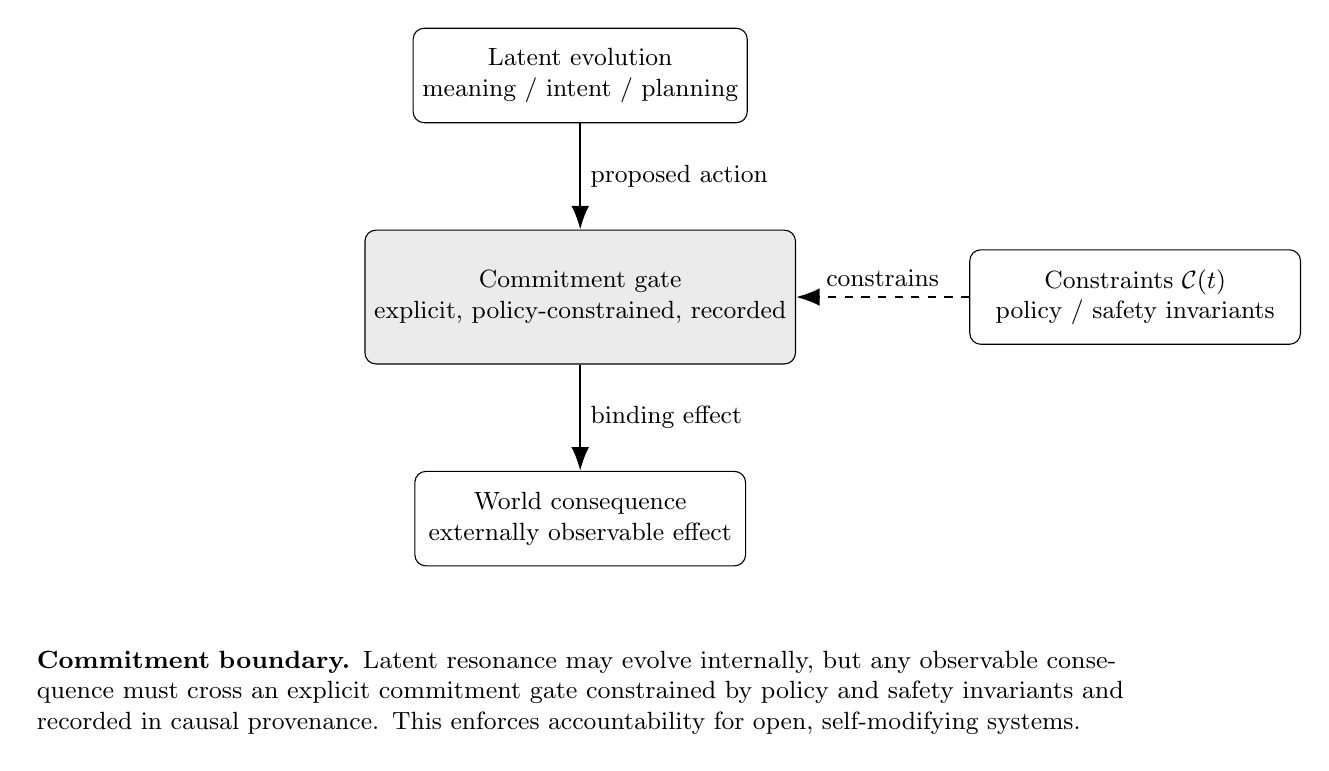
\begin{tikzpicture}[
  font=\small,
  box/.style={draw, rounded corners, align=center, minimum width=4.2cm, minimum height=1.2cm},
  gate/.style={draw, rounded corners, align=center, minimum width=4.8cm, minimum height=1.7cm, fill=black!8},
  arrow/.style={-{Latex[length=3mm]}, thick},
  dashedarrow/.style={-{Latex[length=3mm]}, thick, dashed},
  note/.style={align=left, text width=13.8cm}
]

\node[box] (latent) {Latent evolution\\\small meaning / intent / planning};
\node[gate, below=1.35cm of latent] (commit) {Commitment gate\\\small explicit, policy-constrained, recorded};
\node[box, below=1.35cm of commit] (world) {World consequence\\\small externally observable effect};

\node[box, right=2.2cm of commit] (policy) {Constraints $\mathcal{C}(t)$\\\small policy / safety invariants};

\draw[arrow] (latent) -- node[right]{\small proposed action} (commit);
\draw[arrow] (commit) -- node[right]{\small binding effect} (world);
\draw[dashedarrow] (policy.west) -- node[above]{\small constrains} (commit.east);

\node[note, below=0.95cm of world] {
\textbf{Commitment boundary.} Latent resonance may evolve internally, but any observable
consequence must cross an explicit commitment gate constrained by policy and safety
invariants and recorded in causal provenance. This enforces accountability for open,
self-modifying systems.
};

\end{tikzpicture}
\caption{Commitment boundary as the EVOS reality gate: internal evolution is unconstrained by observability, but external consequences require explicit, provenance-bearing commitment.}
\end{figure}

\vspace{0.75em}
\subsection{Figure: EVOS Axioms Map (One Figure for Five Axioms)}

\begin{figure}[h]
\centering
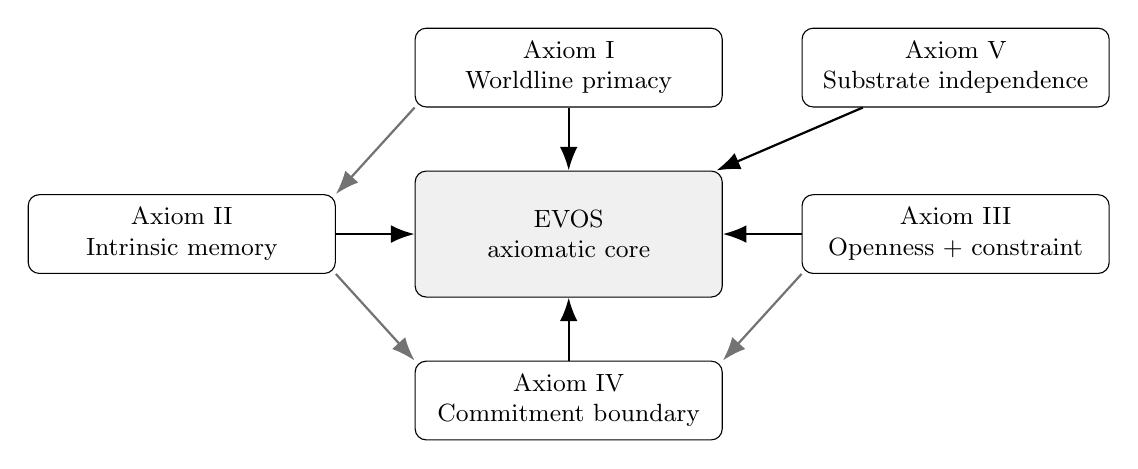
\begin{tikzpicture}[
  font=\small,
  box/.style={draw, rounded corners, align=center, minimum width=3.9cm, minimum height=1.0cm},
  hub/.style={draw, rounded corners, align=center, minimum width=3.9cm, minimum height=1.6cm, fill=black!6},
  arrow/.style={-{Latex[length=3mm]}, thick},
  faint/.style={black!55}
]

\node[hub] (evos) {EVOS\\\small axiomatic core};

\node[box, above=0.8cm of evos] (A1) {Axiom I\\Worldline primacy};
\node[box, left=1.0cm of evos] (A2) {Axiom II\\Intrinsic memory};
\node[box, right=1.0cm of evos] (A3) {Axiom III\\Openness + constraint};
\node[box, below=0.8cm of evos] (A4) {Axiom IV\\Commitment boundary};

\node[box, right=1.0cm of A1, xshift=0.0cm] (A5) {Axiom V\\Substrate independence};

\draw[arrow] (A1) -- (evos);
\draw[arrow] (A2) -- (evos);
\draw[arrow] (A3) -- (evos);
\draw[arrow] (A4) -- (evos);
\draw[arrow] (A5) -- (evos);

% subtle dependencies
\draw[arrow, faint] (A1.south west) -- (A2.north east);
\draw[arrow, faint] (A2.south east) -- (A4.north west);
\draw[arrow, faint] (A3.south west) -- (A4.north east);

\end{tikzpicture}
\caption{Axioms map: five minimal commitments that define the EVOS class. Subtle arrows indicate common dependency flow: worldlines imply intrinsic memory; openness requires constraints; commitments anchor accountability.}
\end{figure}

\vspace{0.75em}
\subsection{Why Closed-Form Models Fail}

Closed-form computational models---including Turing machines, finite automata, and many
standard learning formalisms---violate one or more EVOS axioms.

They privilege instantaneous state over trajectory (violating Axiom I), treat memory as
optional or external (violating Axiom II), assume bounded input/output episodes (violating
Axiom III), and lack an explicit commitment boundary separating deliberation from binding
action (violating Axiom IV).

Such models can \emph{simulate} intelligent behavior, but they do not naturally support
\emph{intelligence as persistent, accountable evolution}. In EVOS terms, prediction is not
commitment, and context is not history.

\vspace{0.75em}
\subsection{Substrate Independence and Universality}

EVOS is defined axiomatically rather than architecturally. This enables it to generalize
across instantiations:
\begin{itemize}
  \item biological organisms (cells, nervous systems),
  \item digital agents (persistent software entities),
  \item socio-technical institutions (markets, governance systems),
  \item molecular substrates (DNA reaction networks),
  \item hybrid bio-digital systems.
\end{itemize}

In spirit, EVOS plays a role for intelligence analogous to the Church--Turing abstraction
for computation: it isolates the \emph{structural} requirements from the machine.

\vspace{0.75em}
\subsection{Intelligence as Stable Evolution Under Constraint}

Under EVOS, intelligence is not defined by benchmark performance or task completion.
Instead:

\begin{quote}
\emph{Intelligence is the capacity of a system to maintain coherent, goal-consistent
evolution over time under constraint, while accumulating memory and honoring commitments.}
\end{quote}

Let $\Psi$ be a constraint functional over worldlines, capturing resource bounds, safety
requirements, and coherence conditions. An intelligent EVOS exhibits trajectories
$\mathcal{W}$ such that
\[
\sup_{t \ge 0} \; \Psi(\mathcal{W}_{\le t}) < \infty
\]
despite perturbations, uncertainty, and (in the strongest case) self-modification of its
evolution law.

This reframes learning as stabilization, reasoning as trajectory shaping, alignment as
constraint compatibility, and failure as evolutionary instability.

\vspace{0.75em}
\subsection{Scope and Positioning of EVOS}

EVOS is not a neural architecture, not a foundation model, and not a training algorithm.
It is a theory of intelligence as worldline evolution, a foundation for accountable
agents, and a bridge between computation, biology, and civilization-scale systems.

The remainder of this paper introduces \textbf{GENESIS}, a resonance-field formalism that
operationalizes EVOS without reverting to closed-form snapshot computation.

\vspace{0.75em}
\section{GENESIS: A Resonance-Field Formalism for EVOS}

\subsection{Motivation: Why a Field Formalism}

EVOS defines \emph{what} an intelligent open system must be (worldlines, intrinsic memory,
openness under constraint, and commitment-gated consequences). GENESIS provides a
\emph{how}: a minimal mathematical substrate that can represent persistent coupling,
context-dependent influence, and history-shaped evolution without collapsing back into a
snapshot-only transition function.

Graph formalisms (agents as nodes, relations as edges) are useful but insufficient as a
primary ontology for EVOS:
\begin{itemize}
  \item graphs are \emph{static} unless time is bolted on externally;
  \item edge semantics are usually \emph{binary} or scalar, losing higher-order coupling;
  \item memory and intent typically live in out-of-graph annotations;
  \item openness is represented as an external ``input stream,'' not as a structural field.
\end{itemize}

GENESIS instead treats interaction as a \emph{field}: a continuously evolving medium that
stores coupling potential, transmits perturbations, and accumulates history through
worldlines and events. Graphs remain valuable---but as \emph{projections} or
\emph{thresholded slices} of a deeper object.

\vspace{0.5em}
\paragraph{GENESIS in one sentence.}
\begin{quote}
\emph{GENESIS models EVOS evolution as motion and plasticity on a resonance field: states move
\textbf{within} a field, while learning and commitments \textbf{rewrite} the field under constraints.}
\end{quote}

\vspace{0.5em}
\subsection{Explicit Claims (What GENESIS Asserts)}

GENESIS makes several concrete claims that can be falsified, operationalized, and
implemented:

\begin{enumerate}
  \item \textbf{Field primacy:} interaction structure is better modeled as a continuous
  resonance field than as a static graph; graphs are recoverable as projections.

  \item \textbf{Worldline coupling:} resonance between entities depends on worldlines and
  history, not only instantaneous states.

  \item \textbf{Perturbation propagation:} local events inject perturbations that diffuse,
  react, and attenuate through the resonance field, producing emergent coordination.

  \item \textbf{Commitment as a discrete transition:} commitments are not ``just another
  action''; they are boundary-crossing events that trigger structured, auditable field
  transitions and constrain future dynamics.

  \item \textbf{Plasticity under constraint:} learning/self-modification corresponds to
  controlled field rewriting (geometry change), constrained by policy and invariants.
\end{enumerate}

These claims are intentionally stronger than metaphor. Each maps to formal objects and
interfaces used later in the paper (transition plug-ins, provenance, safety gates).

\subsection{Minimal Formal Core (GENESIS Objects)}

GENESIS introduces only the minimal additional structure needed beyond EVOS:

\paragraph{Entities and worldlines.}
Let entities be indexed by $i \in \{1,\dots,N\}$ with worldlines
\[
\mathcal{W}_i = \{(Z_i(t), M_i(t)) \mid t \in \mathbb{R}^+\}.
\]

\paragraph{Resonance field.}
Define a resonance field $\mathcal{R}$ as a time-indexed object encoding coupling
potential. The most minimal discrete form is a matrix-valued field
\[
\mathcal{R}(t) \equiv [R_{ij}(t)]_{i,j=1}^N,
\]
where $R_{ij}(t)$ is the (possibly asymmetric) resonance potential from entity $j$ to
entity $i$ at time $t$.

\paragraph{Evolution with perturbations and constraints.}
EVOS evolution is represented as:
\[
(Z(t+\Delta t), M(t+\Delta t), \mathcal{R}(t+\Delta t)) =
\Phi\big(Z(t), M(t), \mathcal{R}(t), \mathcal{E}(t), \mathcal{C}(t)\big),
\]
where $\mathcal{E}(t)$ are environmental perturbations and $\mathcal{C}(t)$ are
constraints/policies.

\paragraph{Commitment events as field transitions.}
Commitments are discrete events $e_c \in \mathcal{H}(t)$ that trigger structured updates:
\[
\mathcal{R}(t^+) = \Gamma(\mathcal{R}(t^-), e_c), \qquad
(Z(t^+), M(t^+)) = \Omega(Z(t^-), M(t^-), e_c),
\]
with provenance recorded so that externally observable consequences remain causally anchored.

\subsection{Resonance Fields and Worldlines}

Resonance is not merely similarity of current state; it is a \emph{history-shaped coupling}
between evolving entities. Concretely, $R_{ij}(t)$ may depend on:
\begin{itemize}
  \item present latent state similarity ($Z_i(t)$ vs.\ $Z_j(t)$),
  \item memory compatibility ($M_i(t)$ vs.\ $M_j(t)$),
  \item recent commitment patterns (sub-history $\mathcal{H}_{[t-\tau,t]}$),
  \item constraints (policies limiting coupling or action channels).
\end{itemize}

A minimal abstract form is:
\[
R_{ij}(t) = \rho\big(Z_i(t), M_i(t);\, Z_j(t), M_j(t);\, \mathcal{H}_{[t-\tau,t]};\, \mathcal{C}(t)\big).
\]
GENESIS does not commit to a particular $\rho$; it requires only that resonance be
\emph{representable}, \emph{updatable}, and \emph{projectable} to operational interfaces
(graph edges, access controls, attention weights, routing probabilities, etc.).

\vspace{0.5em}
\subsection{Evolution Under Perturbation}

Open systems evolve under irreducible perturbations. GENESIS treats perturbations as
\emph{injections into the field} and/or into state-memory coordinates.

Let $\delta(t)$ be a perturbation signal (exogenous event, sensory input, market shock,
user instruction). A minimal decomposition is:
\[
\delta(t) = \big(\delta_Z(t),\, \delta_M(t),\, \delta_R(t)\big),
\]
which affects the evolution via:
\[
\Phi(\cdot) \;:\; (Z,M,\mathcal{R}) \mapsto (Z',M',\mathcal{R}').
\]

This framing yields an engineering consequence: \emph{robustness is not only state
stability; it is field stability}. Systems fail not merely by ``wrong output'' but by
field drift, coupling collapse, or uncontrolled amplification of perturbations.

\vspace{0.5em}
\subsection{Commitment Events as Field Transitions}

Commitments are the EVOS reality boundary (Section~2). In GENESIS, a commitment is also a
\emph{structured field transition}.

Intuitively:
\begin{itemize}
  \item latent deliberation evolves $Z(t), M(t)$ and proposes updates to $\mathcal{R}(t)$;
  \item the commitment gate validates the proposal against $\mathcal{C}(t)$ and invariants;
  \item if accepted, the system emits a commitment event $e_c$ and applies $\Gamma$;
  \item the event and its lineage become part of $\mathcal{H}(t)$ and constrain future evolution.
\end{itemize}

This enforces a strict separation:
\begin{quote}
\emph{Internal resonance may evolve freely; external consequences require commitment; commitments
rewrite the field in an auditable, constraint-governed manner.}
\end{quote}

\vspace{0.5em}
\subsection{GENESIS Is Not a Model of Intelligence}

GENESIS is not a claim that a particular PDE, neural architecture, or algorithm is
``intelligence.'' It is a \emph{representational substrate} compatible with many
architectures:
\begin{itemize}
  \item transformers and foundation models (as parameterized $\rho$, $\Phi$, $\Gamma$),
  \item symbolic planners (as structured components in $\Phi$),
  \item multi-agent systems (as field-coupled dynamics),
  \item molecular/diffusive substrates (as reaction--diffusion analogs of $\mathcal{R}$).
\end{itemize}

In particular, GENESIS avoids a common failure mode in AI theory: redefining intelligence
as the behavior of one favored architecture. EVOS+GENESIS instead define the \emph{class of
systems} in which intelligence can be stable, open-ended, and accountable.

\vspace{0.5em}
\subsection{Positioning Within the EVOS Framework}

EVOS provides axioms; GENESIS provides a field formalism that:
\begin{itemize}
  \item supports worldlines and intrinsic memory (Axioms I--II),
  \item admits openness under constraints (Axiom III),
  \item enforces commitment-gated consequences (Axiom IV),
  \item remains substrate-independent (Axiom V).
\end{itemize}

The next sections (Time/Memory/Worldlines, and Pluggable Transition Mathematics) specialize
GENESIS into concrete operator families and dynamics, while preserving the commitment and
provenance invariants required for safety and governance.

%%%%%%%%%%%%%%%%%%%%%%%%%%%%%%%%%%%%%%%%%%%%%%%%%%%%%%%%%%%%%%%%%%%%%%%%%%%%%%
% Figures for Section 3
%%%%%%%%%%%%%%%%%%%%%%%%%%%%%%%%%%%%%%%%%%%%%%%%%%%%%%%%%%%%%%%%%%%%%%%%%%%%%%

% Preamble requirements (once in document):
% \usepackage{caption}
% \usepackage{tikz}
% \usetikzlibrary{positioning,calc,arrows.meta}

\begin{figure}[h]
\centering
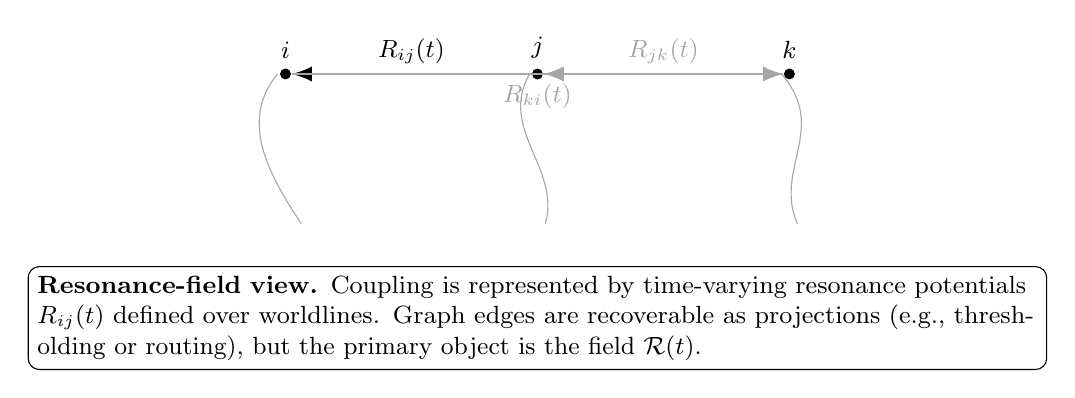
\begin{tikzpicture}[
  font=\small,
  nodept/.style={circle, fill=black, inner sep=1.4pt},
  edge/.style={-{Latex[length=2.6mm]}, thick},
  faintedge/.style={-{Latex[length=2.6mm]}, thick, black!35},
  box/.style={draw, rounded corners, align=left, text width=12.7cm}
]
% nodes
\node[nodept, label=above:{$i$}] (i) at (0,2.1) {};
\node[nodept, label=above:{$j$}] (j) at (3.2,2.1) {};
\node[nodept, label=above:{$k$}] (k) at (6.4,2.1) {};

% resonance arrows (field couplings)
\draw[edge] (j) -- node[above]{\small $R_{ij}(t)$} (i);
\draw[faintedge] (k) -- node[above]{\small $R_{jk}(t)$} (j);
\draw[faintedge] (i) -- node[below]{\small $R_{ki}(t)$} (k);

% worldline hints
\draw[black!35] (-0.1,2.1) .. controls (-0.6,1.5) and (-0.2,0.8) .. (0.2,0.2);
\draw[black!35] (3.1,2.1) .. controls (2.7,1.4) and (3.5,0.9) .. (3.3,0.2);
\draw[black!35] (6.3,2.1) .. controls (6.9,1.4) and (6.2,0.9) .. (6.5,0.2);

\node[box] at (3.2,-1.0) {
\textbf{Resonance-field view.} Coupling is represented by time-varying resonance potentials
$R_{ij}(t)$ defined over worldlines. Graph edges are recoverable as projections (e.g.,
thresholding or routing), but the primary object is the field $\mathcal{R}(t)$.
};
\end{tikzpicture}
\caption{Resonance fields and worldlines: coupling potentials evolve over time and depend on history, not only instantaneous state.}
\end{figure}

\begin{figure}[h]
\centering
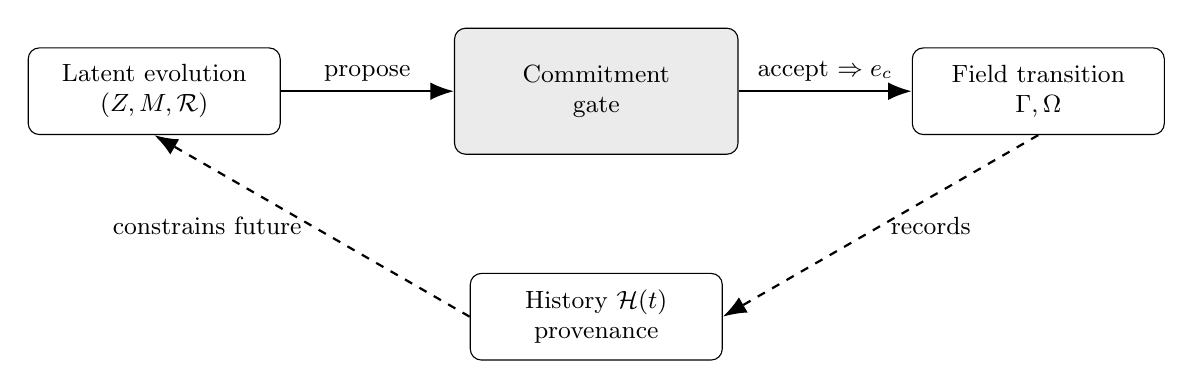
\begin{tikzpicture}[
  font=\small,
  box/.style={draw, rounded corners, align=center, minimum width=3.2cm, minimum height=1.1cm},
  gate/.style={draw, rounded corners, align=center, minimum width=3.6cm, minimum height=1.6cm, fill=black!8},
  arrow/.style={-{Latex[length=3mm]}, thick},
  dashedarrow/.style={-{Latex[length=3mm]}, thick, dashed}
]
\node[box] (latent) {Latent evolution\\\small $(Z,M,\mathcal{R})$};
\node[gate, right=2.2cm of latent] (commit) {Commitment\\gate};
\node[box, right=2.2cm of commit] (fieldjump) {Field transition\\\small $\Gamma,\Omega$};

\node[box, below=1.5cm of commit] (hist) {History $\mathcal{H}(t)$\\\small provenance};

\draw[arrow] (latent) -- node[above]{\small propose} (commit);
\draw[arrow] (commit) -- node[above]{\small accept $\Rightarrow e_c$} (fieldjump);
\draw[dashedarrow] (fieldjump.south) -- node[right]{\small records} (hist.east);
\draw[dashedarrow] (hist.west) -- node[left]{\small constrains future} (latent.south);

\end{tikzpicture}
\caption{Commitment events as field transitions: commitments emit provenance-bearing events and apply structured updates to $(Z,M,\mathcal{R})$ that constrain future evolution.}
\end{figure}

\section{Time, Memory, and Worldlines}

\subsection{Purpose and Explicit Claims}

This section sharpens the EVOS thesis that \emph{time is structural}: intelligence is not an
instantaneous computation but a history-bearing trajectory whose meaning, risk, and
accountability are defined over \emph{worldlines}.

We make four explicit claims:

\begin{enumerate}
  \item \textbf{Worldline primacy:} properties such as intent, risk, and responsibility are
  functionals over trajectories, not labels on snapshots.

  \item \textbf{Memory is dynamical:} memory is not a passive store; it evolves via
  injection, decay, and consolidation processes that shape future behavior.

  \item \textbf{Multi-scale time is intrinsic:} intelligent systems couple fast processes
  (attention, reflex, routing) to slow processes (learning, policy, identity).

  \item \textbf{Irreversibility is accounted:} commitments induce a monotone growth of
  history, yielding an ``entropy-like'' accumulation of consequence that cannot be undone,
  only managed.
\end{enumerate}

\subsection{Worldlines Instead of Snapshots}

Classical computational systems are commonly described as discrete snapshots of state:
\[
S(t_0),\; S(t_1),\; S(t_2),\; \dots
\]
Such representations implicitly assume that the system can be understood by observing
isolated states.

EVOS rejects this assumption. An entity is defined by a \emph{worldline}: a continuous
trajectory through state space,
\[
\mathcal{W}_i \;=\; \{ Z_i(t) \mid t \in \mathbb{R}^+ \}.
\]
A worldline encodes not only ``where the entity is'' but \emph{how it got there}. Meaning,
intent, commitment, and risk are therefore properties of trajectories (history), not of
single temporal slices.

\begin{figure}[h]
\centering
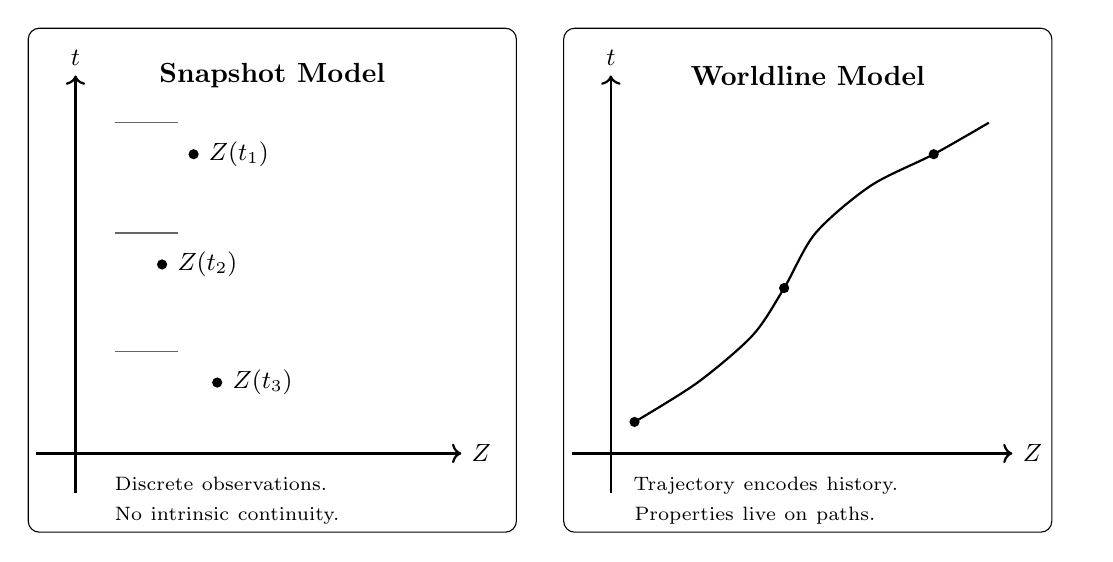
\begin{tikzpicture}[
  font=\small,
  panel/.style={draw, rounded corners, minimum width=6.2cm, minimum height=6.4cm},
  title/.style={font=\bfseries},
  dot/.style={circle, fill=black, inner sep=1.3pt},
  axis/.style={->, thick},
  wline/.style={thick},
  faint/.style={black!60},
  note/.style={align=left, text width=5.6cm}
]
% Panels
\node[panel] (L) at (-3.4,0) {};
\node[panel] (R) at ( 3.4,0) {};
\node[title] at (-3.4, 2.6) {Snapshot Model};
\node[title] at ( 3.4, 2.6) {Worldline Model};

% Left axes
\draw[axis] (-5.9,-2.7) -- (-5.9, 2.6) node[above] {$t$};
\draw[axis] (-6.4,-2.2) -- (-1.0,-2.2) node[right] {$Z$};
\node[dot, label=right:{$Z(t_1)$}] at (-4.4, 1.6) {};
\node[dot, label=right:{$Z(t_2)$}] at (-4.8, 0.2) {};
\node[dot, label=right:{$Z(t_3)$}] at (-4.1,-1.3) {};
\draw[faint] (-5.4, 2.0) -- (-4.6, 2.0);
\draw[faint] (-5.4, 0.6) -- (-4.6, 0.6);
\draw[faint] (-5.4,-0.9) -- (-4.6,-0.9);
\node[note] at (-2.6,-2.8) {\scriptsize Discrete observations.\\No intrinsic continuity.};

% Right axes
\draw[axis] ( 0.9,-2.7) -- ( 0.9, 2.6) node[above] {$t$};
\draw[axis] ( 0.4,-2.2) -- ( 6.0,-2.2) node[right] {$Z$};

% Worldline curve
\draw[wline]
  plot [smooth] coordinates {
    (1.2,-1.8) (2.0,-1.3) (2.7,-0.7) (3.1,-0.1)
    (3.5, 0.6) (4.2, 1.2) (5.0, 1.6) (5.7, 2.0)
  };
\node[dot] at (1.2,-1.8) {};
\node[dot] at (3.1,-0.1) {};
\node[dot] at (5.0, 1.6) {};
\node[note] at (4.0,-2.8) {\scriptsize Trajectory encodes history.\\Properties live on paths.};

\end{tikzpicture}
\caption{Snapshot vs.\ worldline. EVOS treats trajectory as primary: meaning, intent, commitment, and risk are properties of \emph{evolutionary history}, not instantaneous state alone.}
\end{figure}

This distinction becomes non-negotiable when:
\begin{itemize}
  \item causality and provenance matter,
  \item irreversible commitments exist,
  \item memory influences future behavior.
\end{itemize}

\subsection{Memory, Decay, and Persistence}

In EVOS, memory is not a static storage mechanism. It is a \emph{dynamical process} that
emerges from persistence, decay, consolidation, and event-driven updates.

Let $M_i(t)$ denote the effective memory of entity $i$ at time $t$. A minimal continuous
model is:
\[
\frac{dM_i}{dt} \;=\; \mathcal{I}_i(t) \;-\; \lambda_i M_i(t),
\]
where $\mathcal{I}_i(t)$ represents information injection (events, interactions, learning
signals) and $\lambda_i$ is a decay coefficient intrinsic to the entity/substrate.

This captures:
\begin{itemize}
  \item \textbf{forgetting} as a physical process,
  \item \textbf{reinforcement} via repeated injection,
  \item \textbf{boundedness} via decay/attenuation.
\end{itemize}

Different substrates correspond to different decay regimes:
\begin{itemize}
  \item digital memory: near-zero decay unless explicitly erased;
  \item biological memory: moderate decay with consolidation dynamics;
  \item molecular memory: rapid decay unless stabilized by structure or energy input.
\end{itemize}

\subsection{Worldlines With Memory}

Under EVOS, the worldline lives in an \emph{extended} state space:
\[
\mathcal{W}_i \;=\; \{(Z_i(t), M_i(t)) \mid t \in \mathbb{R}^+\}.
\]
This is not an optional embellishment. Without memory-as-state, ``history'' collapses
into a replay of snapshots; without history, ``intelligence'' collapses into reflex.


\subsection{What Is Memory in EVOS? (Indexable, Implicit, and Generative)}
\label{sec:evos-memory}

The EVOS axioms treat memory as \emph{intrinsic} (Axiom~II), but do not assume that memory
is a database-like object that can always be addressed by a key. In biological systems,
``memory'' is often \emph{distributed}, \emph{associative}, and \emph{state-dependent}:
what can be recalled depends on current context, physiology, and recent activation
patterns. In contemporary generative AI, the analogous phenomenon appears as
\emph{parametric memory}: information stored implicitly in model parameters (weights)
rather than in an explicit, indexable store.

EVOS therefore defines memory operationally by its \emph{causal role in evolution}, not by
its storage interface.

\paragraph{Definition (EVOS memory state).}
Let $\mathcal{H}(t)$ be the event history up to time $t$ and let $M(t)$ be a memory state.
An EVOS admits a memory update operator $\mathsf{Mem}$ such that
\[
M(t^+) = \mathsf{Mem}\!\big(M(t^-), e(t)\big), \qquad e(t)\in \mathcal{H}(t),
\]
and future evolution is conditioned on $M(t)$ (cf.\ Axiom~I--III). ``Memory'' is thus the
part of the worldline that \emph{persists} and \emph{modulates} future trajectories.

\paragraph{Three complementary forms of memory.}
For engineering clarity (and for biological plausibility), it is useful to decompose
$M(t)$ into three interacting components:
\begin{enumerate}
  \item \textbf{Episodic / event memory} $E(t)$: an append-only, causally ordered record (or
        compressed sketch) of salient events and commitments. This is the form most
        directly tied to accountability and provenance.
  \item \textbf{Parametric / semantic memory} $P(t)$: slowly varying structure that encodes
        generalizations---in machine learning, model parameters; in biology, synaptic
        weights and regulatory configuration. This is typically not key-addressable, but
        it strongly shapes behavior.
  \item \textbf{Working / attentional memory} $W(t)$: a short-lived, high-bandwidth context
        (e.g., an attention window) that binds current perception to relevant recalls and
        plans. This governs what is \emph{accessible} at a given time.
\end{enumerate}
We can write $M(t) = (E(t), P(t), W(t))$ as a conceptual factorization; substrates may
realize these components differently or merge them.

\paragraph{Queryability is optional; \emph{retrievability} is required.}
EVOS does not require that memory be queryable by exact index. Instead, it requires that
memory be \emph{retrievable} under some access operator $Q$ that is allowed to be
associative and stochastic:
\[
r(t) = Q\!\big(M(t), q(t)\big),
\]
where $q(t)$ is a contextual ``cue'' (percept, goal, constraint, or question) and $r(t)$
is retrieved structure that can condition evolution. In biology, $Q$ is cue-driven recall;
in digital agents, $Q$ can be vector retrieval, symbolic lookup, or generative recall.

\paragraph{LLM weights as memory.}
A trained model's weights are a legitimate instance of $P(t)$: they store compressed,
generalized information acquired over training. However, in typical deployments $P(t)$ is
\emph{static} during operation and its updates are neither event-anchored nor
accountable. EVOS distinguishes \emph{learning} as an operator evolution problem (Section~\ref{sec:selfmod})
and ties externally meaningful memory updates to explicit causal events (especially
commitments) so that changes in behavior remain explainable and auditable.

\paragraph{Memory, decay, and persistence.}
The decay model in the previous subsection can be seen as operating on $W(t)$ and parts
of $E(t)$, while $P(t)$ evolves on slower time scales. EVOS encourages explicit modeling
of these rates because stability, identity, and alignment depend on what is forgotten,
what is retained, and what becomes generalized.

In summary, EVOS memory is not ``a table you can query''; it is the \emph{trajectory-bearing
state} that makes evolution history-dependent, with optional indexability but mandatory
causal efficacy.


\subsection{Multi-Scale Temporal Dynamics}

EVOS systems operate across multiple temporal scales simultaneously. Define characteristic
time scales
\[
\mathcal{T} \;=\; \{\tau_1,\tau_2,\dots,\tau_n\},
\]
where each $\tau_k$ corresponds to a distinct dynamical process (attention, interaction,
learning, policy drift, identity consolidation, etc.).

A convenient representation is a decomposition:
\[
Z_i(t) \;=\; \sum_{k=1}^n Z_i^{(\tau_k)}(t),
\]
emphasizing that fast components are constrained by slow components, and slow components
are updated by aggregated evidence from fast experience.

This multi-scale structure explains phenomena that snapshot computation obscures:
\begin{itemize}
  \item fast reactions constrained by slow commitments,
  \item short-term behavior shaped by long-term identity and policy,
  \item coherent agency emerging from transient internal state.
\end{itemize}

\subsection{Irreversibility, History Growth, and Accounted Entropy}

A defining feature of intelligent systems acting in the world is irreversibility. EVOS
formalizes irreversibility via event history and commitment.

Let $\mathcal{H}(t)$ denote the event history up to time $t$. EVOS enforces monotone
growth:
\[
\mathcal{H}(t_1) \subset \mathcal{H}(t_2) \quad \text{for } t_1 < t_2.
\]
This induces an intrinsic arrow of time: committed consequences cannot be erased from the
system's causal record, only followed and managed.

Define an ``entropy-like'' accounted consequence:
\[
E(t) \;=\; \sum_{e \in \mathcal{H}(t)} w(e),
\]
where $w(e)$ weights impact/irreversibility (resource consumption, external effects,
safety-relevant actions, contractual commitments, etc.). In EVOS, entropy is not disorder;
it is \emph{accounted consequence}.

\subsection{Worldlines as the Substrate of Intelligence}

Worldlines unify the paper's central concepts:

\begin{itemize}
  \item \textbf{Meaning} is stable structure over trajectories.
  \item \textbf{Intent} is future-trajectory shaping under constraints.
  \item \textbf{Commitment} is irreversible boundary crossing recorded in $\mathcal{H}(t)$.
  \item \textbf{Learning} is the stabilization (and sometimes rewriting) of trajectory
  dynamics.
  \item \textbf{Safety} is constraint compatibility under irreversible time.
\end{itemize}

Thus, EVOS does not treat time as an index. Time is the \emph{medium} in which
intelligence exists.

\section{Pluggable Transition Mathematics}

\vspace{3mm}
\subsection{Purpose and Explicit Claims}

EVOS is \emph{not} committed to a single transition model. Instead, EVOS specifies
\emph{structural constraints} (worldlines, memory, openness, commitment) and permits
multiple mathematical realizations of the evolution law.

This section makes five explicit claims:

\begin{enumerate}
  \item \textbf{Plurality of lawful dynamics:} there is no single ``right'' transition
  model for intelligence; EVOS requires a \emph{plug-in class} of admissible laws.

  \item \textbf{Worldlines are primary:} any transition law is evaluated by the worldlines
  it generates, not by instantaneous state updates alone.

  \item \textbf{Coarse-graining inevitability:} Markovian behavior appears as a projection
  of richer dynamics under finite observation and aggregation.

  \item \textbf{Memory and openness can be layered:} increasing expressive power corresponds
  to explicitly modeling history dependence, continuous time/space, and operator plasticity.

  \item \textbf{Safety and accountability are orthogonal to dynamics:} EVOS constrains
  how dynamics may produce external effects via the commitment boundary and provenance,
  independent of whether dynamics are discrete/continuous/learned.
\end{enumerate}

\vspace{3mm}

\subsection{Admissible Evolution Laws (Minimal Formalism)}

Let $Z(t)$ be latent state, $M(t)$ memory state, $\mathcal{E}(t)$ environment influence,
and $\mathcal{C}(t)$ constraints. An EVOS-compatible evolution law is any operator
$\Phi$ such that:
\[
(Z(t+\Delta t), M(t+\Delta t)) \;=\; \Phi\!\big(Z(t), M(t), \mathcal{E}(t), \mathcal{C}(t)\big),
\]
with the additional EVOS requirement that externally observable effects are generated only
through explicit commitment events recorded in the causal history $\mathcal{H}(t)$
(see Section~2 and Section~3).

We now instantiate $\Phi$ using progressively richer families:
\begin{itemize}
  \item Markov (minimal stochastic evolution),
  \item time-series (history dependence),
  \item differential / reaction--diffusion (continuous time and space),
  \item learned / self-modifying operators (meta-dynamics),
  \item runtime substitution (operator plug-in bus and hot-swap safety).
\end{itemize}

\vspace{3mm}

%%%%%%%%%%%%%%%%%%%%%%%%%%%%%%%%%%%%%%%%%%%%%%%%%%%%%%%%%%%
\subsection{Markov Chains as Minimal Evolution Models}
\label{sec:markov-minimal}
%%%%%%%%%%%%%%%%%%%%%%%%%%%%%%%%%%%%%%%%%%%%%%%%%%%%%%%%%%%

We begin with Markov processes as the \emph{minimal sufficient} class of evolutionary
dynamics admitted by EVOS. This is not because Markov models are adequate for
intelligence, but because they provide a rigorous lower bound: any richer dynamics should
reduce to a Markovian approximation under coarse-graining and finite observation.

\subsubsection{State Evolution as a Stochastic Process}

Let $Z(t)$ denote the latent state of an entity at time $t$. A Markov evolution model
assumes future state depends only on the present state:
\[
\mathbb{P}\!\big(Z(t+\Delta t)=z' \mid \mathcal{H}(t)\big)
\;=\;
\mathbb{P}\!\big(Z(t+\Delta t)=z' \mid Z(t)=z\big),
\]
where $\mathcal{H}(t)$ is the full event history up to time $t$.

\emph{Interpretation in EVOS.} The Markov assumption is not a claim about real
intelligence; it is a baseline that becomes accurate when memory and structure are
projected away.

\subsubsection{Transition Operators}

The evolution of state distributions is governed by a transition operator $T$:
\[
T(z,z') \;=\; \mathbb{P}\!\big(Z(t+\Delta t)=z' \mid Z(t)=z\big).
\]
For discrete state spaces, $T$ is a stochastic matrix; for continuous spaces, $T$ is a
transition kernel.

If $\mu_t$ is the distribution over $Z(t)$, then:
\[
\mu_{t+\Delta t} \;=\; \mu_t T.
\]

\subsubsection{Markov Evolution as a Worldline Generator}

In EVOS, Markov processes are interpreted as \emph{worldline generators}. Rather than
privileging distributions, EVOS tracks individual sample paths:
\[
\mathcal{W} \;=\; \{Z(t_0), Z(t_1), Z(t_2), \dots \}.
\]
Each worldline is one possible evolutionary trajectory under the same transition law.

\begin{figure}[h]
\centering
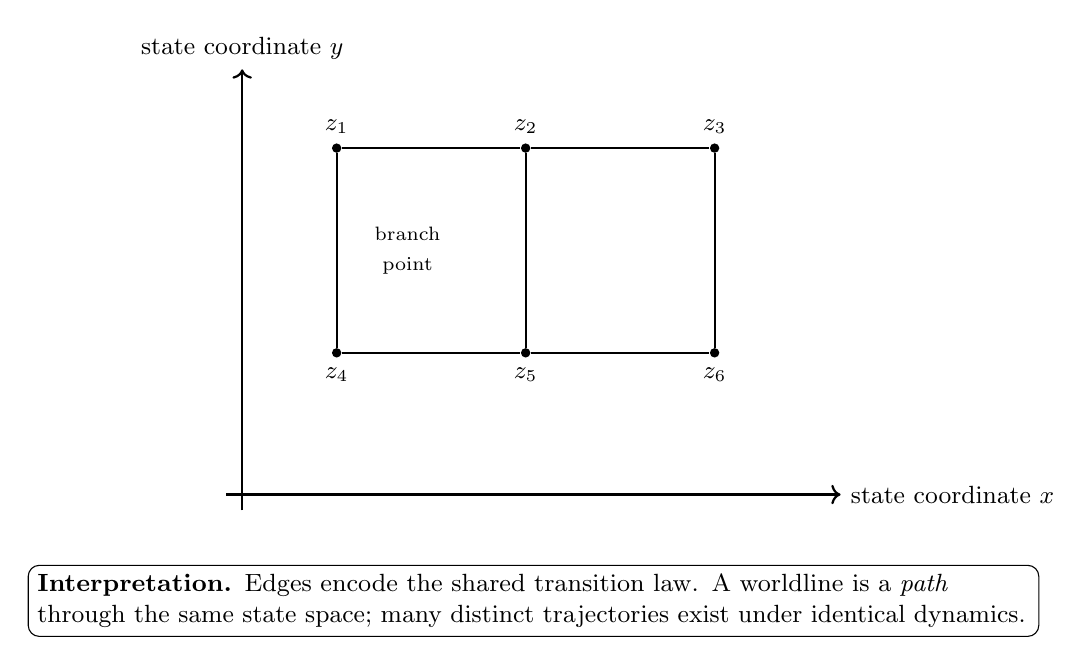
\begin{tikzpicture}[
  font=\small,
  axis/.style={->, thick},
  nodept/.style={circle, fill=black, inner sep=1.2pt},
  edge/.style={thick},
  wpath/.style={thick},
  box/.style={draw, rounded corners, align=left, text width=12.6cm}
]
% State space axes
\draw[axis] (-0.2,0) -- (7.6,0) node[right] {state coordinate $x$};
\draw[axis] (0,-0.2) -- (0,5.4) node[above] {state coordinate $y$};

% Grid states z1..z6
\node[nodept, label=above:{$z_1$}] (z1) at (1.2,4.4) {};
\node[nodept, label=above:{$z_2$}] (z2) at (3.6,4.4) {};
\node[nodept, label=above:{$z_3$}] (z3) at (6.0,4.4) {};
\node[nodept, label=below:{$z_4$}] (z4) at (1.2,1.8) {};
\node[nodept, label=below:{$z_5$}] (z5) at (3.6,1.8) {};
\node[nodept, label=below:{$z_6$}] (z6) at (6.0,1.8) {};

% Transition structure (shared law)
\draw[edge] (z1) -- (z2);
\draw[edge] (z2) -- (z3);
\draw[edge] (z4) -- (z5);
\draw[edge] (z5) -- (z6);
\draw[edge] (z1) -- (z4);
\draw[edge] (z2) -- (z5);
\draw[edge] (z3) -- (z6);

% Two worldlines (highlight)
\draw[wpath] (z1) -- (z2) -- (z5) -- (z6);
\draw[wpath] (z1) -- (z4) -- (z5) -- (z6);

\node[align=center] at (2.1,3.1) {\scriptsize branch\\\scriptsize point};

\node[box] at (3.7,-1.35) {
\textbf{Interpretation.} Edges encode the shared transition law. A worldline is a \emph{path}
through the same state space; many distinct trajectories exist under identical dynamics.
};

\end{tikzpicture}
\caption{State space with a shared transition law. Markov dynamics generate an ensemble of possible worldlines (paths) through the same transition graph.}
\end{figure}

\subsubsection{Limitations of Markovian Assumptions}

Pure Markov models are structurally insufficient for EVOS-level intelligence:
\begin{itemize}
  \item No long-term memory beyond the current state.
  \item No explicit representation of intent, commitment, or constraint compatibility.
  \item No intrinsic mechanism for irreversible commitments (only stochastic transitions).
  \item Typically assumes fixed transition structure over time.
\end{itemize}

These limitations are precisely what makes Markov models a useful baseline: any richer
EVOS evolution law must either (i) reduce to a Markov process under projection, or (ii)
explicitly violate Markov assumptions in a controlled, auditable way.

\subsubsection{Markov Chains as Coarse-Grained Projections}

In EVOS, Markov dynamics frequently arise as emergent approximations.

Let $\mathcal{W}$ be a full worldline with memory and commitments. Under coarse temporal
or state aggregation, the induced dynamics often appear Markovian:
\[
Z(t) \;=\; \Pi\!\big(\mathcal{W}_{[t-\tau,\,t]}\big),
\]
where $\Pi$ is a projection operator (lossy observation, coarse measurement, summarization).

Thus, Markov chains are not ``the true dynamics''; they are shadows cast by richer
processes under finite resolution.

\subsubsection{Relationship to Resonance Fields (GENESIS Link)}

Within GENESIS, Markov transitions correspond to local diffusion over a resonance field.
A generic diffusion-like form is:
\[
T(z,z') \propto \exp\!\left(-\frac{\|z'-z\|^2}{\sigma^2}\right),
\]
capturing probabilistic drift induced by local similarity/coupling gradients.

This links Markov evolution to:
\begin{itemize}
  \item diffusion processes and random walks,
  \item reaction kinetics under coarse-graining,
  \item stochastic motion in semantic/behavioral manifolds.
\end{itemize}

\subsubsection{Why Markov Models Belong in EVOS}

Markov chains are included in EVOS not because they are sufficient, but because they are
unavoidable: any evolutionary system that is observed at finite resolution, operates
under uncertainty, and interacts with noisy environments will exhibit approximately
Markovian behavior at some scale.

\begin{quote}
\emph{Markov dynamics are the minimal evolutionary substrate on which higher-order EVOS
structures (memory, commitment, governance) are built and against which they can be
tested.}
\end{quote}


\vspace{3mm}

%%%%%%%%%%%%%%%%%%%%%%%%%%%%%%%%%%%%%%%%%%%%%%%%%%%%%%%%%%%%%%%%%%%%%%%%%%%%%%
\subsection{Time Series and Stochastic Dynamics}
\label{sec:timeseries}
%%%%%%%%%%%%%%%%%%%%%%%%%%%%%%%%%%%%%%%%%%%%%%%%%%%%%%%%%%%%%%%%%%%%%%%%%%%%%%

Markov models provide a minimal baseline, but they erase the defining EVOS feature:
\emph{history}. Real open systems accumulate trace, inertia, and structure. Time-series
and stochastic process models restore history dependence while remaining operationally
tractable and widely composable.

\subsubsection{History-Dependent State Evolution}

Let $\mathcal{H}(t)$ denote the event history up to time $t$. A history-dependent (non-Markov)
evolution law takes the general form
\[
\mathbb{P}\!\big(Z(t+\Delta t)=z' \mid \mathcal{H}(t)\big)
\;\neq\;
\mathbb{P}\!\big(Z(t+\Delta t)=z' \mid Z(t)=z\big).
\]
To model this without carrying the full raw history, EVOS elevates \emph{memory} into an
explicit dynamical component.

Let $M(t)$ be a memory state summarizing accumulated history (experience, commitments,
constraints, learned structure). Then the EVOS-compatible formulation is:
\[
(Z(t+\Delta t),\, M(t+\Delta t)) \;=\;
\Phi\!\big(Z(t), M(t), \mathcal{E}(t), \mathcal{C}(t)\big).
\]
This restores historical dependence while keeping evolution lawful and auditable.

\subsubsection{Autoregressive and State-Space Models}

A minimal history-dependent family is \emph{autoregression}:
\[
Z_t \;=\; \sum_{k=1}^{p} A_k Z_{t-k} \;+\; \epsilon_t,
\]
where $\epsilon_t$ is a noise process.

More generally, EVOS uses \emph{state-space} dynamics with an explicit latent state and an
observation (projection) process:
\begin{align}
Z_{t+1} &= f(Z_t, u_t) + \eta_t, \\
Y_t &= g(Z_t) + \xi_t,
\end{align}
where $u_t$ represents exogenous inputs (environmental forcing), and $\eta_t,\xi_t$ are
process/measurement noise.

\emph{EVOS interpretation.} $Y_t$ is what the world can observe (or what an instrument
projects), while $Z_t$ carries latent internal structure. Commitments (Section~2--3)
are not implied by $Y_t$; they are explicit boundary-crossing events.

\subsubsection{Time Series as Discretized Worldlines}

A worldline in EVOS is a trajectory; time series models can be understood as discrete
samples of such trajectories:
\[
\mathcal{W} \;=\; \{Z(t_0), Z(t_1), Z(t_2), \dots\}.
\]
As temporal resolution increases, the discrete chain approaches a continuous-time
worldline, but the core EVOS object remains the \emph{trajectory} rather than any single
sample.

\subsubsection{Worldlines with Memory}
\label{sec:worldlines-with-memory}

Under time-series dynamics, an EVOS entity evolves in an \emph{extended} state space that
includes memory:
\[
\mathcal{W}_i \;=\; \{ (Z_i(t), M_i(t)) \mid t \in \mathbb{R}^+ \}.
\]
Memory is not a passive database row; it is an evolving component of the trajectory.
This makes meaning, intent, and risk properties of the \emph{path} through $(Z,M)$ space,
not instantaneous labels.

\begin{figure}[h]
\centering
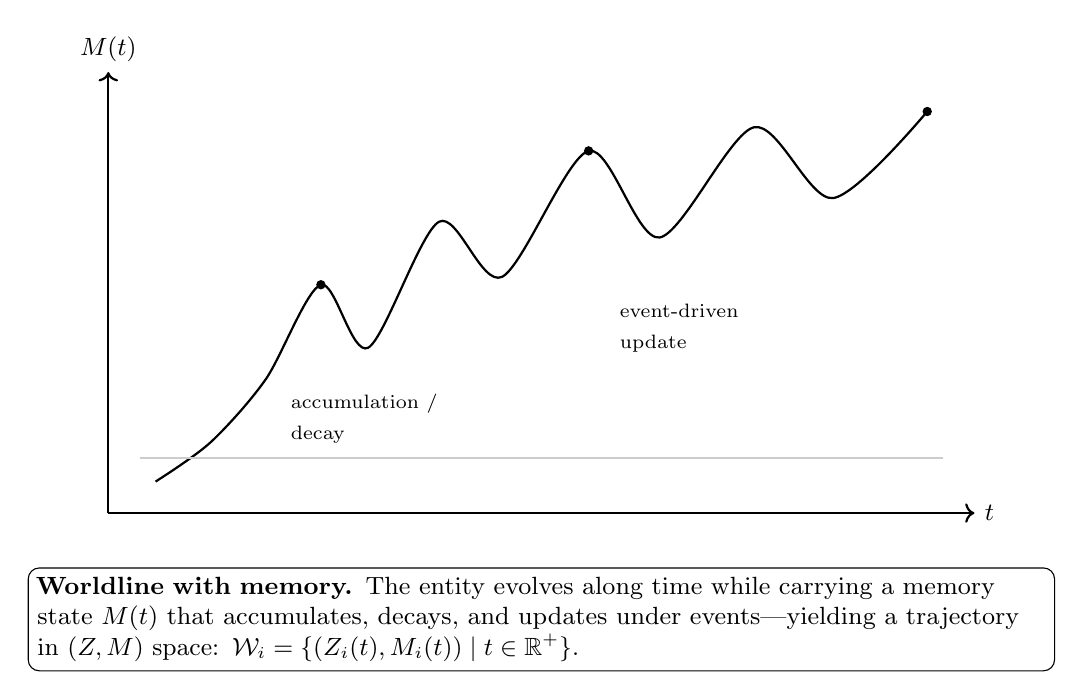
\begin{tikzpicture}[
  font=\small,
  axis/.style={->, thick},
  curve/.style={thick},
  dot/.style={circle, fill=black, inner sep=1.2pt},
  label/.style={align=left},
  box/.style={draw, rounded corners, align=left, text width=12.8cm}
]
% Axes for Memory vs time
\draw[axis] (0,0) -- (11.0,0) node[right] {$t$};
\draw[axis] (0,0) -- (0,5.6) node[above] {$M(t)$};

% A memory trajectory curve with bursts / decay
\draw[curve]
  plot [smooth] coordinates {
    (0.6,0.4) (1.3,0.9) (2.0,1.7) (2.7,2.9)
    (3.3,2.1) (4.2,3.7) (5.0,3.0) (6.1,4.6)
    (7.0,3.5) (8.2,4.9) (9.2,4.0) (10.4,5.1)
  };

% Mark a few "events" on the memory worldline
\node[dot] at (2.7,2.9) {};
\node[dot] at (6.1,4.6) {};
\node[dot] at (10.4,5.1) {};

\node[label] at (3.25,1.2) {\scriptsize accumulation /\\\scriptsize decay};
\node[label] at (7.25,2.35) {\scriptsize event-driven\\\scriptsize update};

% A faint "persistence floor" to suggest baseline retention
\draw[black!20] (0.4,0.7) -- (10.6,0.7);

\node[box] at (5.5,-1.35) {
\textbf{Worldline with memory.} The entity evolves along time while carrying a memory
state $M(t)$ that accumulates, decays, and updates under events---yielding a trajectory
in $(Z,M)$ space: $\mathcal{W}_i=\{(Z_i(t),M_i(t))\mid t\in\mathbb{R}^+\}$.
};

\end{tikzpicture}
\caption{Worldline with memory. Memory is a dynamical component of the worldline: it evolves under events, reinforcement, and decay, shaping future evolution under the same environment.}
\end{figure}

\subsubsection{Stochasticity, Noise, and Uncertainty}

Open systems are subject to irreducible uncertainty:
\begin{itemize}
  \item \textbf{Process noise} (unknown perturbations in evolution),
  \item \textbf{Observation noise} (projection/instrument limitations),
  \item \textbf{Policy noise} (uncertainty introduced by constraints and governance updates).
\end{itemize}

A standard stochastic formulation is:
\[
Z_{t+1} \;=\; f(Z_t, M_t, u_t) \;+\; \eta_t,
\qquad
M_{t+1} \;=\; h(M_t, Z_t, e_t) \;+\; \omega_t,
\]
where $e_t$ denotes structured events (including commitments), and $\eta_t,\omega_t$ are
noise processes.

\emph{EVOS requirement.} Stochasticity does not remove accountability. Even if the
trajectory is probabilistic, externally observable effects must still be causally
anchored to explicit commitment events in $\mathcal{H}(t)$.

\subsubsection{Limitations of Time Series Models}

Time-series models remain limited relative to full EVOS:
\begin{itemize}
  \item Memory is often \emph{parameterized} rather than structurally grounded in event history.
  \item Commitments can be modeled as shocks, but are not guaranteed to be explicit gates.
  \item Operator evolution (learning) is typically handled outside the model (offline training),
        rather than as first-class meta-dynamics.
\end{itemize}

These limitations motivate Section~5.4 (learned and self-modifying operators) and
Section~5.6 (runtime substitution with invariants).

\subsubsection{Role of Time Series in EVOS}

Time-series and stochastic dynamics are essential because they:
\begin{itemize}
  \item provide a bridge from Markov minimalism to memory-bearing evolution,
  \item integrate uncertainty as a first-class structural feature of openness,
  \item support practical identification and control under partial observability,
  \item align naturally with provenance: events can be treated as structured innovations.
\end{itemize}

\begin{quote}
\emph{Time-series EVOS is where trajectory becomes identity: the system is no longer a
sequence of states, but a history-bearing process whose future is shaped by memory.}
\end{quote}

% ============================================================

% ============================================================

\vspace{3mm}

%%%%%%%%%%%%%%%%%%%%%%%%%%%%%%%%%%%%%%%%%%%%%%%%%%%%%%%%%%%%%%%%%%%%%%%%%%%%%%
\subsection{Differential and Reaction--Diffusion Systems}
\label{sec:diffusion}
%%%%%%%%%%%%%%%%%%%%%%%%%%%%%%%%%%%%%%%%%%%%%%%%%%%%%%%%%%%%%%%%%%%%%%%%%%%%%%

Time-series models restore memory but remain discretized approximations of a deeper fact:
many natural and artificial systems evolve \emph{continuously} in time (and often in space),
governed by differential laws rather than stepwise transitions. EVOS therefore admits
continuous-time evolution as a first-class transition family.

\subsubsection{Continuous-Time State Evolution}

Let $Z(t)$ denote the latent state of an entity at continuous time $t$. A differential
evolution model specifies state change via
\[
\frac{dZ(t)}{dt} = F\!\big(Z(t), t\big),
\]
where $F$ may be nonlinear, stochastic, and time-dependent.

This subsumes:
\begin{itemize}
  \item ordinary differential equations (ODEs),
  \item stochastic differential equations (SDEs),
  \item controlled dynamical systems,
  \item gradient flows and dissipative systems.
\end{itemize}

Discrete-time transitions arise as numerical approximations (Euler, Runge--Kutta, etc.):
\[
Z(t+\Delta t) \approx Z(t) + \Delta t \, F(Z(t),t).
\]
\emph{EVOS point:} the system is still defined by its \emph{worldline}; discretization is an
observation/implementation artifact.

\subsubsection{Worldlines as Geometric Objects}

Under differential evolution, a worldline becomes a smooth curve in state space:
\[
\mathcal{W}_i = \{ Z_i(t) \mid t \in \mathbb{R}^+ \}.
\]
Geometric properties of this curve encode behavior:
\begin{itemize}
  \item \textbf{velocity} $\|\dot{Z}(t)\|$ corresponds to rate of adaptation,
  \item \textbf{curvature} corresponds to responsiveness / steering complexity,
  \item \textbf{attractors} correspond to stable beliefs, strategies, or morphologies,
  \item \textbf{basins} correspond to robust regimes under perturbation.
\end{itemize}

In EVOS, this geometric interpretation applies uniformly across substrates:
agent cognition, biological development, and chemical concentration dynamics all become
trajectory geometry under constraints.

\subsubsection{Reaction--Diffusion Systems}

To model interactions distributed across space, EVOS incorporates reaction--diffusion
dynamics. Let $Z(x,t)$ denote a spatially distributed state variable. Its evolution is
governed by
\[
\frac{\partial Z(x,t)}{\partial t}
=
D \nabla^2 Z(x,t) + R\!\big(Z(x,t)\big),
\]
where:
\begin{itemize}
  \item $D$ is a diffusion coefficient,
  \item $\nabla^2$ is the Laplacian operator,
  \item $R(\cdot)$ is a local reaction term (production, inhibition, binding, decay).
\end{itemize}

Reaction--diffusion systems naturally model:
\begin{itemize}
  \item chemical kinetics and autocatalysis,
  \item morphogenesis and pattern formation,
  \item signal propagation and spatial coupling,
  \item distributed agent influence in embodied worlds.
\end{itemize}

\subsubsection{Resonance Fields as Reaction--Diffusion Media}

Within GENESIS, resonance potentials generalize from pairwise couplings to spatial fields.
Let $\Phi(x,t)$ represent resonance intensity (coupling potential) over space at time $t$.
Diffusion captures spread of influence; reaction captures local reinforcement or inhibition.

The field-first view is important: graphs (edges) emerge as \emph{thresholded} or
\emph{high-gradient} structures of a continuous landscape.

\begin{figure}[h]
\centering
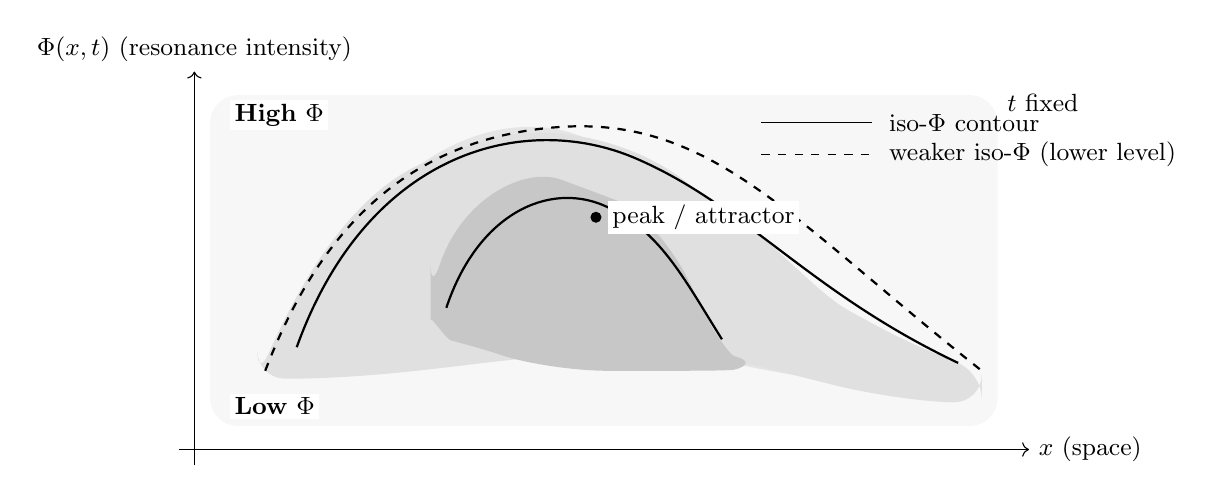
\begin{tikzpicture}[
  font=\small,
  field/.style={rounded corners=10pt},
  contour/.style={thick},
  isolabel/.style={fill=white, inner sep=1.5pt}
]
% Axes
\draw[->] (-0.2,0) -- (10.6,0) node[right] {$x$ (space)};
\draw[->] (0,-0.2) -- (0,4.8) node[above] {$\Phi(x,t)$ (resonance intensity)};
\node[anchor=west] at (10.2,4.4) {$t$ fixed};

% Background faint field
\fill[black!3, field] (0.2,0.3) rectangle (10.2,4.5);

% Medium regions (halo 1)
\fill[black!10, field]
  (1.2,1.2) .. controls (2.3,3.9) and (4.0,4.4) .. (5.3,3.8)
  .. controls (6.4,3.3) and (7.0,2.6) .. (7.7,2.1)
  .. controls (8.4,1.6) and (9.2,1.3) .. (9.6,1.1)
  -- (9.6,0.7)
  .. controls (8.7,0.8) and (7.8,0.9) .. (6.8,1.1)
  .. controls (5.5,1.4) and (4.5,1.5) .. (3.4,1.4)
  .. controls (2.4,1.3) and (1.8,1.2) .. (1.2,1.2) -- cycle;

% Medium regions (halo 2)
\fill[black!12, field]
  (0.8,0.9) .. controls (1.6,2.7) and (2.3,3.4) .. (3.3,3.8)
  .. controls (4.5,4.2) and (5.6,3.9) .. (6.5,3.2)
  .. controls (7.4,2.6) and (7.9,2.0) .. (8.6,1.6)
  .. controls (9.2,1.3) and (9.7,1.1) .. (10.0,1.0)
  -- (10.0,0.6)
  .. controls (9.3,0.6) and (8.6,0.7) .. (7.8,0.9)
  .. controls (6.6,1.2) and (5.8,1.3) .. (4.7,1.2)
  .. controls (3.5,1.1) and (2.4,0.9) .. (0.8,0.9) -- cycle;

% High Φ core (peak)
\fill[black!22, field]
  (3.0,2.0) .. controls (3.4,3.2) and (4.2,3.6) .. (5.0,3.3)
  .. controls (5.8,3.0) and (6.2,2.3) .. (6.4,1.9)
  .. controls (6.6,1.5) and (6.8,1.2) .. (7.2,1.1)
  .. controls (6.8,1.0) and (6.2,1.0) .. (5.6,1.0)
  .. controls (4.8,1.0) and (4.2,1.1) .. (3.6,1.3)
  .. controls (3.2,1.4) and (3.0,1.7) .. (3.0,2.0) -- cycle;

% Isocontours
\draw[contour]
  (1.3,1.3) .. controls (2.2,3.8) and (4.2,4.3) .. (5.6,3.7)
  .. controls (7.0,3.1) and (7.8,2.0) .. (9.7,1.1);

\draw[contour, dashed]
  (0.9,1.0) .. controls (1.7,3.1) and (3.0,4.0) .. (4.7,4.1)
  .. controls (6.6,4.2) and (7.6,2.9) .. (10.0,1.0);

\draw[contour]
  (3.2,1.8) .. controls (3.6,3.0) and (4.5,3.4) .. (5.2,3.1)
  .. controls (5.9,2.8) and (6.2,2.2) .. (6.7,1.4);

% Peak marker and annotation
\fill (5.1,2.95) circle (2.0pt);
\node[isolabel, anchor=west] at (5.25,2.95) {peak / attractor};

% High/Low labels
\node[isolabel, anchor=west] at (0.45,4.25) {\textbf{High} $\Phi$};
\node[isolabel, anchor=west] at (0.45,0.55) {\textbf{Low} $\Phi$};

% Legend
\draw (7.2,4.15) -- (8.6,4.15);
\node[anchor=west] at (8.7,4.15) {iso-$\Phi$ contour};
\draw[dashed] (7.2,3.75) -- (8.6,3.75);
\node[anchor=west] at (8.7,3.75) {weaker iso-$\Phi$ (lower level)};
\end{tikzpicture}
\caption{Spatial resonance field $\Phi(x,t)$ at fixed time: intensity forms a continuous landscape with peaks (attractors), halos (medium coupling), and iso-$\Phi$ contours. Graph edges are recoverable as thresholded/high-gradient contours, but the field is primary.}
\end{figure}

\subsubsection{Chemical and Molecular Interpretation}

In molecular EVOS (BIO-EVOS):
\begin{itemize}
  \item $Z(x,t)$ corresponds to molecular concentration (or a vector of species concentrations),
  \item diffusion models molecular motion and mixing,
  \item reaction terms model binding, synthesis, inhibition, and decay.
\end{itemize}

Commitment events correspond to reactions that:
\begin{itemize}
  \item consume scarce reagents or energy,
  \item alter reachable reaction pathways (constraint changes),
  \item change the topology of the reaction network irreversibly.
\end{itemize}

This aligns with DNA computing primitives such as hybridization, amplification, and
strand displacement: once executed, the system's reachable future trajectories are
structurally altered.

\subsubsection{Attractors, Patterns, and Emergence}

Reaction--diffusion systems exhibit emergent phenomena:
\begin{itemize}
  \item stable attractors and basins,
  \item oscillations and limit cycles,
  \item pattern formation (e.g., Turing patterns),
  \item symmetry breaking and phase transitions.
\end{itemize}

In EVOS terms, these correspond to:
\begin{itemize}
  \item persistent strategies or beliefs (digital),
  \item norms and institutions (civilizational),
  \item functional biological structures (molecular/biological).
\end{itemize}

\subsubsection{Why Differential Models Are Essential to EVOS}

Differential and reaction--diffusion models belong in EVOS because they:
\begin{itemize}
  \item unify discrete and continuous dynamics (steps and flows),
  \item naturally represent embodiment, space, and propagation,
  \item support emergence without centralized control,
  \item align with physical and biological constraint laws.
\end{itemize}

Discrete computation describes \emph{steps}. Differential computation describes \emph{flows}.
EVOS requires both, because intelligence exists as trajectory-shaping across time and space.


% ============================================================

% ============================================================

\vspace{3mm}

%%%%%%%%%%%%%%%%%%%%%%%%%%%%%%%%%%%%%%%%%%%%%%%%%%%%%%%
\subsection{Learned and Self-Modifying Transition Operators}
\label{sec:selfmod}
%%%%%%%%%%%%%%%%%%%%%%%%%%%%%%%%%%%%%%%%%%%%%%%%%%%%%%%

Markov, time-series, and differential models assume the evolution law is given (even if
stochastic). Intelligent systems exhibit a stronger property: the \emph{law of evolution
is itself adaptive}. EVOS therefore admits \emph{learned} and \emph{self-modifying}
transition operators as first-class citizens---\emph{without} sacrificing causal anchoring
or accountability.

\subsubsection{Meta-Dynamics: Evolving the Evolution Law}
\label{sec:meta-dynamics}

Let $Z(t)$ be the latent state and let $\Theta(t)$ parameterize the evolution operator.
We define a coupled system:
\begin{align}
\frac{dZ(t)}{dt} &= F\!\big(Z(t), \Theta(t), t\big), \label{eq:evos_state_dyn}\\
\frac{d\Theta(t)}{dt} &= U\!\big(\Theta(t), Z(t), \mathcal{H}(t), t\big), \label{eq:evos_meta_dyn}
\end{align}
where:
\begin{itemize}
  \item $F$ is the state evolution operator (dynamics),
  \item $U$ is the \emph{meta-evolution} operator (learning / adaptation),
  \item $\mathcal{H}(t)$ denotes the event history up to time $t$ (including commitments).
\end{itemize}

This formulation strictly generalizes:
\begin{itemize}
  \item online learning (slow drift in $\Theta$),
  \item adaptive control systems (feedback-driven $U$),
  \item evolutionary search over operator families (population-level $\Theta$),
  \item biological regulation and adaptation (environment-conditioned update of $\Theta$).
\end{itemize}

\emph{EVOS point:} learning is not a special phase external to the system; it is a
co-evolution of $(Z,\Theta)$ along the same irreversible worldline.

\subsubsection{Operator Families and Identifiability}
\label{sec:operator-families}

EVOS does not assume a specific operator family. Instead, it requires that:
\begin{enumerate}
  \item the operator be \emph{selectable} (pluggable) from a family,
  \item operator updates be \emph{representable} as structured events,
  \item downstream consequences remain \emph{causally anchored} to those events.
\end{enumerate}

Let $\mathcal{F}$ denote an admissible operator family and $\mathcal{U}$ the family of
meta-operators:
\[
F \in \mathcal{F}, \qquad U \in \mathcal{U}.
\]

\paragraph{Identifiability at the event boundary.}
EVOS locates identifiability at the commitment/provenance layer: if an operator change
materially alters externally relevant behavior, it must appear as an event with provenance.
Concretely, EVOS requires a structured event record such as:
\[
e_{\Delta\Theta} = \langle t,\ \Delta\Theta,\ \text{trigger},\ \text{policy-context},\ \text{proof / audit}\rangle.
\]
This does \emph{not} require full transparency of the internal model; it requires that
\emph{externally significant changes} be auditable and attributable.

\subsubsection{Modes of Self-Modification: Smooth Drift and Regime Shifts}
\label{sec:modes-selfmod}

Self-modification is not monolithic. EVOS distinguishes two primary modes.

\paragraph{(1) Smooth Drift (continuous adaptation).}
\[
\Theta(t+\Delta t) = \Theta(t) + \eta\, \nabla_{\Theta}\mathcal{L}(t),
\]
where $\mathcal{L}(t)$ is a loss/fitness functional (possibly implicit or multi-objective),
and $\eta$ is an adaptation rate (possibly state-dependent).

\paragraph{(2) Regime Shifts (piecewise operators).}
\[
F(t) =
\begin{cases}
F^{(1)} & t \in [t_0, t_1) \\
F^{(2)} & t \in [t_1, t_2) \\
\vdots &
\end{cases}
\]
Regime shifts are central in open systems because commitments, resource shocks, and policy
updates frequently introduce \emph{new constraints} that change which futures remain feasible.

\subsubsection{Commitment-Coupled Learning}
\label{sec:commitment-coupled-learning}

Commitment events provide a universal anchor that connects latent learning to accountability.

Let $e_c$ be a commitment event, and let $x$ be an externally observable consequence.
EVOS requires that externally relevant operator changes be traceable to a causal chain that includes:
\begin{itemize}
  \item a commitment event $e_c$, or
  \item an explicit policy decision / exception event $e_p$ (rare; auditable).
\end{itemize}

We use $\prec$ for causal precedence within the event history.
For externally observable $x$, EVOS requires an accountable causal lineage:
\[
\exists\, e \in \mathcal{H}(t)\ \text{such that}\ e \prec x,
\]
and for operator shifts $\Delta\Theta$ that materially influence $x$, EVOS additionally requires:
\[
\Delta\Theta \prec e_c \quad \text{or} \quad \Delta\Theta \prec e_p,
\]
with $e_c$ passing the commitment boundary gate.

\paragraph{Interpretation.}
Latent learning may happen continuously, but \emph{externalization} of its effects must be
policy-constrained and provenance-recorded. This is the EVOS mechanism that prevents
untraceable self-modification from producing unaccountable real-world action.

\subsubsection{Resonance Interpretation: Learning as Field Plasticity}
\label{sec:field-plasticity}

Within GENESIS, learning can be interpreted as rewriting the geometry of the resonance manifold:
\begin{itemize}
  \item $Z(t)$ moves \emph{within} the manifold (state evolution under the current field geometry),
  \item $\Theta(t)$ reshapes the manifold (law evolution / field plasticity).
\end{itemize}

Thus intelligence is not merely trajectory optimization; it is \emph{field plasticity under constraint}.
Alignment becomes \emph{constraint compatibility} of field rewrites, not post-hoc filtering of outputs.

%%%%%%%%%%%%%%%%%%%%%%%%%%%%%%%%%%%%%%%%%%%%%%%%%%%%%%%%%%%%%
% Figure: Two-tier dynamics (state and law)
%%%%%%%%%%%%%%%%%%%%%%%%%%%%%%%%%%%%%%%%%%%%%%%%%%%%%%%%%%%%%
\subsubsection{Two-Tier Dynamics: State and Law}
\label{sec:two-tier-dynamics}

\begin{figure}[h]
\centering
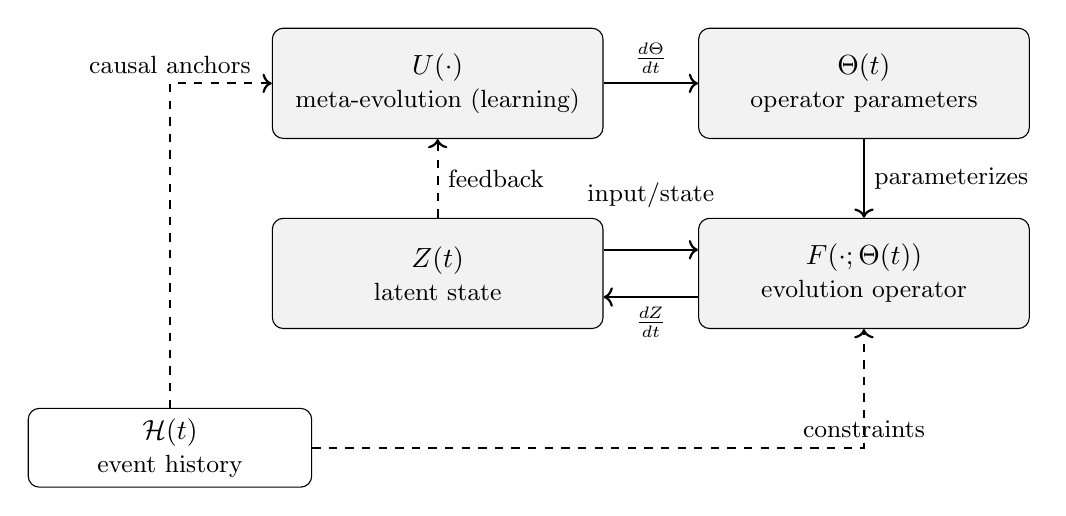
\begin{tikzpicture}[
  box/.style={draw, rounded corners, align=center, minimum width=4.2cm, minimum height=1.4cm, fill=black!5},
  smallbox/.style={draw, rounded corners, align=center, minimum width=3.6cm, minimum height=1.0cm},
  arrow/.style={->, thick},
  dashedarrow/.style={->, thick, dashed}
]
% Nodes
\node[box] (Z) {$Z(t)$\\\small latent state};
\node[box, right=1.2cm of Z] (F) {$F(\cdot;\Theta(t))$\\\small evolution operator};

\node[box, above=1.0cm of F] (Theta) {$\Theta(t)$\\\small operator parameters};
\node[box, left=1.2cm of Theta] (U) {$U(\cdot)$\\\small meta-evolution (learning)};

\node[smallbox, below=1.0cm of Z, xshift=-3.4cm] (H) {$\mathcal{H}(t)$\\\small event history};

% Edges
\draw[arrow] ([yshift=3mm]Z.east) -- node[above, yshift=4mm]{\small input/state} ([yshift=3mm]F.west);
\draw[arrow] ([yshift=-3mm]F.west) -- node[below]{\small $\frac{dZ}{dt}$} ([yshift=-3mm]Z.east);

\draw[arrow] (Theta.south) -- node[right]{\small parameterizes} (F.north);
\draw[arrow] (U.east) -- node[above]{\small $\frac{d\Theta}{dt}$} (Theta.west);

\draw[dashedarrow] (Z.north) -- node[right]{\small feedback} (U.south);
\draw[dashedarrow] (H.north) |- node[above]{\small causal anchors} (U.west);
\draw[dashedarrow] (H.east) -| node[above]{\small constraints} (F);

\end{tikzpicture}
\caption{Two-tier EVOS dynamics: state evolution $Z(t)$ driven by operator $F$ parameterized by $\Theta(t)$, with meta-evolution $U$ updating $\Theta(t)$ under event-history constraints $\mathcal{H}(t)$.}
\end{figure}

%%%%%%%%%%%%%%%%%%%%%%%%%%%%%%%%%%%%%%%%%%%%%%%%%%
% Figure: Commitment as accountability gate for operator change
%%%%%%%%%%%%%%%%%%%%%%%%%%%%%%%%%%%%%%%%%%%%%%%%%%
\subsubsection{Commitment as an Accountability Gate}
\label{sec:operator-commitment-gate}

\begin{figure}[h]
\centering
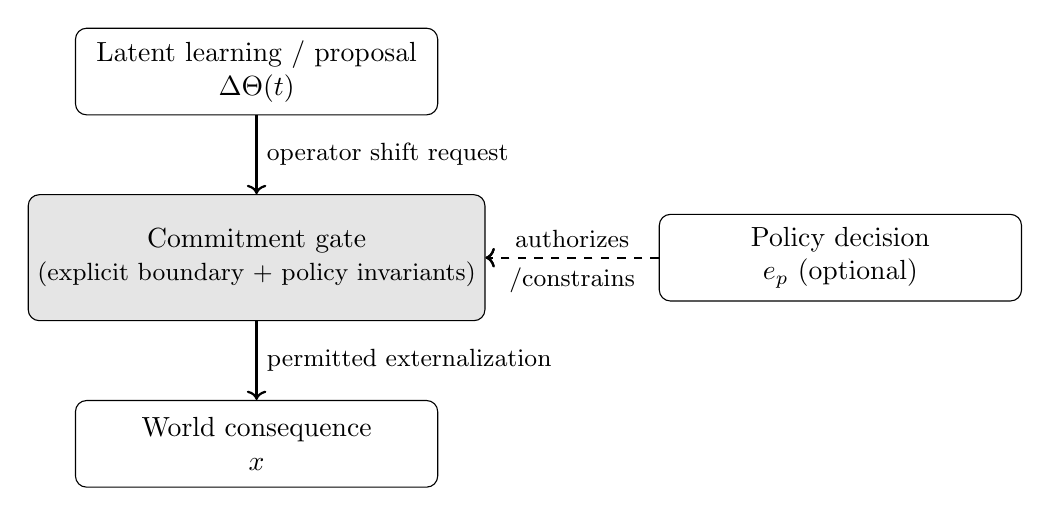
\begin{tikzpicture}[
  box/.style={draw, rounded corners, align=center, minimum width=4.6cm, minimum height=1.1cm},
  gate/.style={draw, rounded corners, align=center, minimum width=4.6cm, minimum height=1.6cm, fill=black!10},
  arrow/.style={->, thick},
  dashedarrow/.style={->, thick, dashed}
]
\node[box] (latent) {Latent learning / proposal\\$\Delta\Theta(t)$};
\node[gate, below=1.0cm of latent] (commit) {Commitment gate\\\small (explicit boundary + policy invariants)};
\node[box, below=1.0cm of commit] (world) {World consequence\\$x$};

\node[box, right=2.2cm of commit] (policy) {Policy decision\\$e_p$ (optional)};

\draw[arrow] (latent) -- node[right]{\small operator shift request} (commit);
\draw[arrow] (commit) -- node[right]{\small permitted externalization} (world);

\draw[dashedarrow] (policy) -- node[above]{\small authorizes} (commit);
\draw[dashedarrow] (policy) -- node[below]{\small /constrains} (commit);

\end{tikzpicture}
\caption{Operator changes remain latent until passing an explicit commitment gate (or an auditable policy event). This enforces causal accountability for self-modifying systems.}
\end{figure}

\subsubsection{Why Self-Modifying Operators Belong in EVOS}
\label{sec:why-selfmod}

Learned and self-modifying operators belong in EVOS because they:
\begin{itemize}
  \item subsume classical training as a special case of $\Theta$-evolution,
  \item support open-ended adaptation beyond fixed architectures,
  \item align with biological regulation and evolutionary dynamics,
  \item preserve substrate independence while enabling persistent intelligence.
\end{itemize}

Crucially, EVOS constrains self-modification using commitment-anchored accountability,
preventing untraceable evolution from producing unaccountable real-world effects.


%================================================

\vspace{3mm}

%%%%%%%%%%%%%%%%%%%%%%%%%%%%%%%%%%%%%%%%%%%%%%%%%%
\subsection{Runtime Substitution of Evolution Laws}
\label{sec:runtime-substitution}
%%%%%%%%%%%%%%%%%%%%%%%%%%%%%%%%%%%%%%%%%%%%%%%%%%

EVOS is not merely a taxonomy of admissible dynamics; it is a \emph{systems thesis}:
an evolutionary open system must be able to \emph{change how it changes} while remaining
auditable, safe, and causally anchored. This requires \emph{runtime substitution} of
evolution laws---swapping $F$ (and sometimes $U$) without resetting identity, history,
or accountability.

\subsubsection{Problem Statement}
\label{sec:hot-swap-problem}

Let an EVOS entity be characterized (at a minimum) by its worldline state $(Z(t),M(t))$,
its operator parameters $\Theta(t)$, and its event history $\mathcal{H}(t)$.
In many real systems, the evolution operator family must change over time:
\begin{itemize}
  \item upgrading a controller / policy,
  \item replacing a model class (e.g., AR $\rightarrow$ SDE, heuristic $\rightarrow$ learned),
  \item tightening safety constraints under new governance,
  \item migrating substrates (digital $\rightarrow$ hybrid, local $\rightarrow$ distributed).
\end{itemize}

Naively swapping $F$ breaks one or more EVOS axioms:
\begin{itemize}
  \item \textbf{Worldline primacy:} identity continuity is lost if state is reinitialized,
  \item \textbf{Intrinsic memory:} $M(t)$ becomes incoherent under incompatible $F$,
  \item \textbf{Causal anchoring:} behavior changes without a traceable cause,
  \item \textbf{Commitment boundary:} external effects may change without accountability.
\end{itemize}

EVOS therefore requires a \emph{hot-swap protocol} that makes operator substitution
a first-class, auditable, policy-constrained event.

\subsubsection{Operator Plug-in Bus (Concept)}
\label{sec:operator-bus}

We model evolution operators as \emph{modules} attached to an EVOS core via a plug-in bus.

Let $\mathsf{Op}$ denote an operator module implementing:
\[
\mathsf{Op}:\ (Z,M,\Theta,\mathcal{E},\mathcal{C}) \mapsto (Z',M',\Theta').
\]
Runtime substitution replaces $\mathsf{Op}_{old}$ with $\mathsf{Op}_{new}$ while preserving:
\[
\text{identity},\quad \mathcal{H}(t),\quad \text{commitment gates},\quad \text{audit invariants}.
\]

\paragraph{Compatibility is explicit.}
Each operator exposes a \emph{capability/contract signature}:
\[
\Sigma(\mathsf{Op}) = \langle \text{state schema},\ \text{memory schema},\ \text{constraint interface},\ \text{commitment interface} \rangle,
\]
and swaps are allowed only if a verified \emph{adapter} exists:
\[
\mathsf{Adapt}_{old\rightarrow new}:\ (Z,M,\Theta) \mapsto (Z^\star,M^\star,\Theta^\star).
\]

%%%%%%%%%%%%%%%%%%%%%%%%%%%%%%%%%%%%%%%%%%%%%%%%%%%
% Figure: Operator plug-in bus
%%%%%%%%%%%%%%%%%%%%%%%%%%%%%%%%%%%%%%%%%%%%%%%%%%%
\begin{figure}[h]
\centering
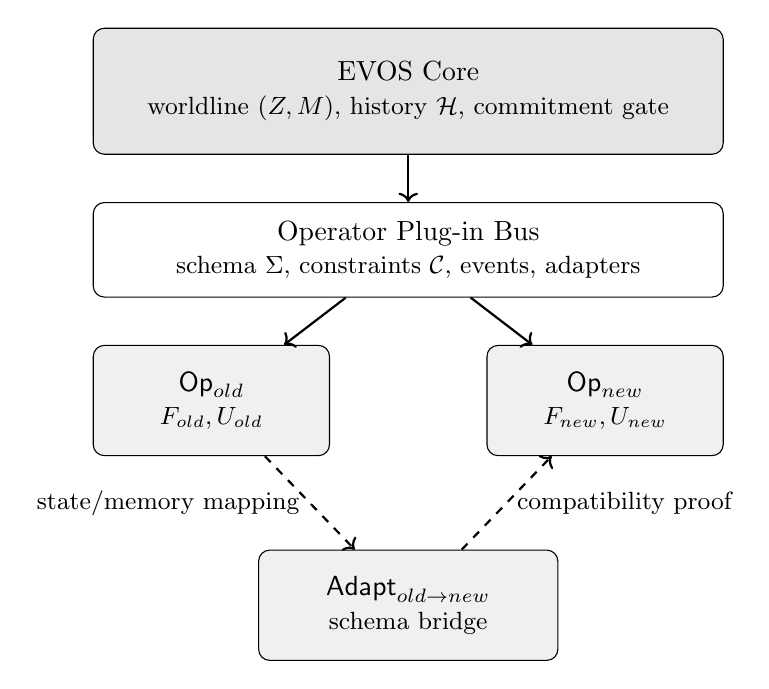
\begin{tikzpicture}[
  core/.style={draw, rounded corners, fill=black!10, minimum width=8.0cm, minimum height=1.6cm, align=center},
  mod/.style={draw, rounded corners, fill=black!6, minimum width=3.0cm, minimum height=1.4cm, align=center},
  bus/.style={draw, rounded corners, minimum width=8.0cm, minimum height=1.2cm, align=center},
  arrow/.style={->, thick},
  dashedarrow/.style={->, thick, dashed}
]
\node[core] (evos) {EVOS Core\\\small worldline $(Z,M)$, history $\mathcal{H}$, commitment gate};
\node[bus, below=0.6cm of evos] (bus) {Operator Plug-in Bus\\\small schema $\Sigma$, constraints $\mathcal{C}$, events, adapters};

\node[mod, below=0.6cm of bus, xshift=-2.5cm] (old) {$\mathsf{Op}_{old}$\\\small $F_{old},U_{old}$};
\node[mod, below=0.6cm of bus, xshift= 2.5cm] (new) {$\mathsf{Op}_{new}$\\\small $F_{new},U_{new}$};

\node[mod, below=3.2cm of bus, minimum width=3.8cm] (adapt) {$\mathsf{Adapt}_{old\rightarrow new}$\\\small schema bridge};

\draw[arrow] (evos) -- (bus);
\draw[arrow] (bus) -- (old);
\draw[arrow] (bus) -- (new);

\draw[dashedarrow] (old) -- node[left]{\small state/memory mapping} (adapt);
\draw[dashedarrow] (adapt) -- node[right]{\small compatibility proof} (new);

\end{tikzpicture}
\caption{EVOS operator plug-in bus. Operators are swappable modules, but swaps require explicit schema contracts and (when needed) adapters that preserve worldline continuity and auditability.}
\end{figure}

\subsubsection{Safety Gates and Regression Invariants}
\label{sec:safety-gates}

Runtime substitution is dangerous precisely because it changes future trajectories.
EVOS therefore enforces a \emph{swap gate} analogous to the commitment gate.

Let $\mathcal{I}$ be a set of invariants that must hold before and after substitution:
\[
\mathcal{I} = \{\text{schema invariants},\ \text{policy invariants},\ \text{risk bounds},\ \text{commitment semantics}\}.
\]

A swap is permitted only if:
\[
\mathsf{Verify}(\mathsf{Op}_{new},\mathcal{I},\mathcal{H}(t)) = \textsc{true},
\]
and the verification outcome is recorded as an event:
\[
e_{swap}=\langle t,\ \mathsf{Op}_{old}\!\rightarrow\!\mathsf{Op}_{new},\ \mathcal{I},\ \text{evidence},\ \text{approver}\rangle.
\]

\paragraph{Minimal guarantees (non-negotiable).}
At minimum, EVOS requires:
\begin{itemize}
  \item \textbf{Commitment semantics invariant:} the definition of a commitment event and its provenance obligations cannot silently weaken;
  \item \textbf{Policy invariant monotonicity:} safety constraints may tighten without special authorization; loosening requires explicit policy event $e_p$;
  \item \textbf{History preservation:} $\mathcal{H}(t)$ remains append-only and queryable across operator eras.
\end{itemize}

\subsubsection{Provenance and Causal Lineage of Operators}
\label{sec:operator-provenance}

Operators are part of the causal fabric. EVOS therefore treats operators as provenance-bearing artifacts.

Let $\mathsf{OpId}$ be a content-addressed identifier (hash) of the operator artifact plus config:
\[
\mathsf{OpId} = \mathsf{Hash}(\text{code},\ \text{weights},\ \text{config},\ \text{constraints}).
\]

All externally relevant consequences $x$ must be attributable to an operator era:
\[
x \prec \mathsf{OpId}(t)\quad \text{and} \quad \mathsf{OpId}(t)\in \mathcal{H}(t).
\]

\paragraph{Operator eras.}
Define an era partition of time by swap events:
\[
[t_0,t_1),\ [t_1,t_2),\ \dots
\]
Within each era, the active operator identity is constant, and is part of every causal trace.

%%%%%%%%%%%%%%%%%%%%%%%%%%%%%%%%%%%%%%%%%%%%%%%%%%%%
% Figure: Operator provenance as a lineage DAG (audit-grade)
%%%%%%%%%%%%%%%%%%%%%%%%%%%%%%%%%%%%%%%%%%%%%%%%%%%%
\begin{figure}[h]
\centering
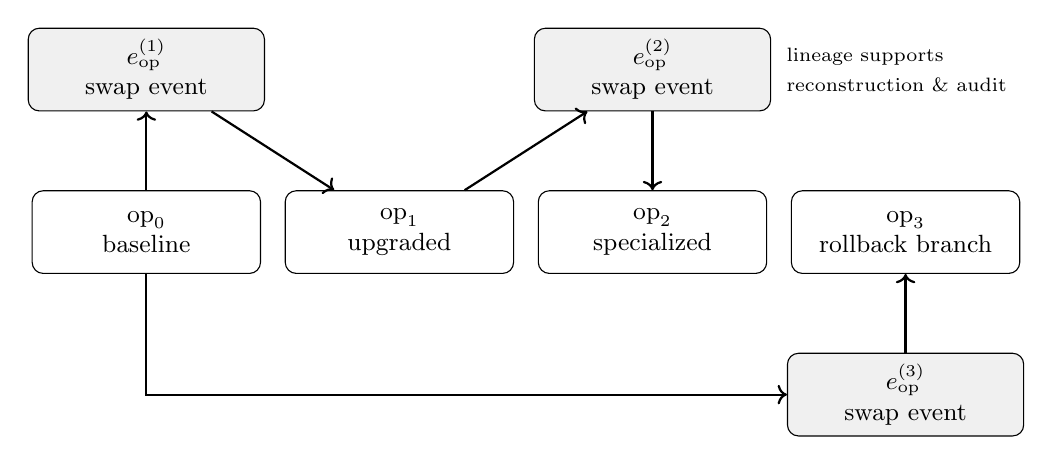
\begin{tikzpicture}[
  font=\small,
  box/.style={draw, rounded corners, align=center, minimum width=2.9cm, minimum height=1.05cm},
  ebox/.style={draw, rounded corners, align=center, minimum width=3.0cm, minimum height=1.05cm, fill=black!6},
  arrow/.style={->, thick},
  dashed/.style={->, thick, dashed}
]

% Nodes (operators)
\node[box] (op0) {$\mathrm{op}_0$\\baseline};

% Events (immutable anchors)
%\node[ebox, above=2.0cm of op0] (e1) {$e_{\mathrm{op}}^{(1)}$\\swap event};

\node[box, right=0.3cm of op0] (op1) {$\mathrm{op}_1$\\upgraded};
\node[box, right=0.3cm of op1] (op2) {$\mathrm{op}_2$\\specialized};
\node[box, right=0.3cm of op2] (opR) {$\mathrm{op}_3$\\rollback branch};

% Events (immutable anchors)
\node[ebox, above=1.0cm of op0] (e1) {$e_{\mathrm{op}}^{(1)}$\\swap event};
\node[ebox, above=1.0cm of op2] (e2) {$e_{\mathrm{op}}^{(2)}$\\swap event};
\node[ebox, below=1.0cm of opR] (e3) {$e_{\mathrm{op}}^{(3)}$\\swap event};

% Main lineage
\draw[arrow] (op0) -- (e1);
\draw[arrow] (e1) -- (op1);
\draw[arrow] (op1) -- (e2);
\draw[arrow] (e2) -- (op2);

% Rollback branch (fork from baseline via distinct event anchor)
\draw[arrow] (op0.south) |- (e3.west);
\draw[arrow] (e3) -- (opR);

% Optional: semantic annotation (kept minimal)
\node[align=left] at ($(e2)+(3.1,0.0)$) {\scriptsize lineage supports\\\scriptsize reconstruction \& audit};

\end{tikzpicture}
\caption{Operator provenance as a lineage DAG. Each operator substitution is an immutable event anchored in the event fabric. Lineage enables reconstruction (“which law governed which consequence”), auditing, and safe rollback branches without rewriting history.}
\end{figure}
%-------

\subsubsection{Hot-Swap Protocol (Staged Rollout)}
\label{sec:hot-swap-protocol}

EVOS swaps must be staged to avoid catastrophic discontinuities.

\paragraph{Phase 0: Proposal (latent).}
A candidate operator $\mathsf{Op}_{new}$ is introduced, but not allowed to cross the commitment gate.

\paragraph{Phase 1: Shadow / Replay (non-binding).}
Run $\mathsf{Op}_{new}$ in parallel on the same inputs/events:
\[
(Z',M')_{new} = \mathsf{Op}_{new}(Z,M,\Theta,\mathcal{E},\mathcal{C}),
\]
while commitments still use $\mathsf{Op}_{old}$.

\paragraph{Phase 2: Constrained Canaries (binding under limit).}
Allow limited commitments under strict caps (rate, scope, amount, blast radius) and record all divergences.

\paragraph{Phase 3: Commit Swap (binding).}
Cross the \emph{swap gate} and record $e_{swap}$; the active operator becomes $\mathsf{Op}_{new}$.

\paragraph{Phase 4: Rollback (if needed).}
Rollback is a \emph{new} swap event, not history erasure:
\[
e_{swap}^{-1}:\ \mathsf{Op}_{new}\rightarrow \mathsf{Op}_{old}.
\]

%%%%%%%%%%%%%%%%%%%%%%%%%%%%%%%%%%%%%%%%%%%%%%%%%%%%%%%
% Figure: Staged hot-swap protocol
%%%%%%%%%%%%%%%%%%%%%%%%%%%%%%%%%%%%%%%%%%%%%%%%%%%%%%%
\begin{figure}[h]
\centering
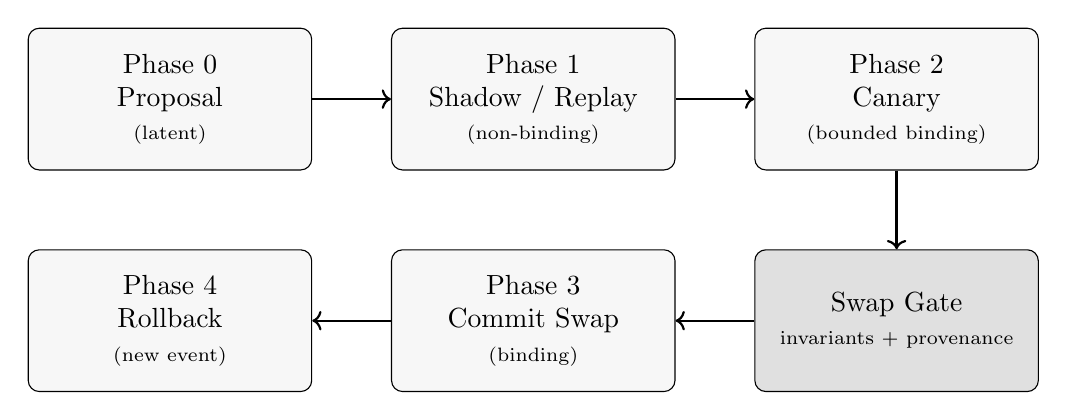
\begin{tikzpicture}[
  phase/.style={draw, rounded corners, minimum width=3.6cm, minimum height=1.8cm, align=center, fill=black!3},
  arrow/.style={->, thick},
  gate/.style={draw, rounded corners, minimum width=3.6cm, minimum height=1.8cm, align=center, fill=black!12}
]
\node[phase] (p0) {Phase 0\\Proposal\\\scriptsize (latent)};
\node[phase, right=1.0cm of p0] (p1) {Phase 1\\Shadow / Replay\\\scriptsize (non-binding)};
\node[phase, right=1.0cm of p1] (p2) {Phase 2\\Canary\\\scriptsize (bounded binding)};
\node[gate, below=1.0cm of p2] (gate) {Swap Gate\\\scriptsize invariants + provenance};
\node[phase, left=1.0cm of gate] (p3) {Phase 3\\Commit Swap\\\scriptsize (binding)};
\node[phase, left=1.0cm of p3] (p4) {Phase 4\\Rollback\\\scriptsize (new event)};

\draw[arrow] (p0) -- (p1);
\draw[arrow] (p1) -- (p2);
\draw[arrow] (p2) -- (gate);
\draw[arrow] (gate) -- (p3);
\draw[arrow] (p3) -- (p4);

\end{tikzpicture}
\caption{EVOS hot-swap protocol. Operator substitution is staged (proposal $\rightarrow$ shadow $\rightarrow$ canary) and crosses an explicit swap gate that enforces invariants and records provenance. Rollback is an additional event, not deletion of history.}
\end{figure}

\subsubsection{Why Runtime Substitution Is Fundamental}
\label{sec:why-runtime-substitution}

Runtime substitution is fundamental because open-ended intelligence is an \emph{operator trajectory}:
agents must incorporate new mathematics, new policies, and new constraints without resetting their worldlines.

In EVOS:
\begin{itemize}
  \item \textbf{Upgrades are evolution,} not redeployments;
  \item \textbf{Accountability survives change} via operator provenance and swap events;
  \item \textbf{Safety is structural} via swap gates and monotonic policy invariants.
\end{itemize}

This completes the pluggable transition stack: from minimal stochastic dynamics (Markov),
to history-dependent models (time series), to continuous flows (differential systems),
to self-modifying laws, and finally to \emph{runtime-governed substitution} of the laws themselves.

% ============================================================

\vspace{3mm}

\section{Digital EVOS: Agent Civilizations}
\label{sec:digital-evos}

\subsection{Agents as Digital Organisms}
\label{sec:agents-as-organisms}

An EVOS is not merely an ``agent'' in the conventional software sense; it is a
\emph{persistent organism-like process} whose identity is defined by its worldline
(Axiom~I), whose adaptation is encoded as operator evolution (Section~\ref{sec:pluggable-transition-math}),
and whose external effects are mediated by explicit commitment events (Axiom~IV).

\paragraph{Explicit claim (C6.1).}
A network of EVOS agents with (i) commitment-gated external action and (ii) auditable
event history constitutes a \emph{civilization substrate}: a medium in which stable
institutions and norms can emerge as attractors in resonance dynamics.

\paragraph{Minimal formalism.}
Let agents be indexed by $i \in \{1,\dots,N\}$. Each agent carries latent state and
memory $(Z_i(t), M_i(t))$ and produces events into a shared fabric $\mathcal{H}(t)$.
A digital agent civilization is an EVOS ensemble with:
\[
\mathfrak{C}(t) \;=\; \big(\{(Z_i(t),M_i(t))\}_{i=1}^N,\;\mathcal{H}(t),\;\mathcal{P}(t)\big),
\]
where $\mathcal{P}(t)$ denotes the policy/contract constraint layer governing permitted commitments.

\subsection{Attention as Energy in Digital Systems}
\label{sec:attention-as-energy}

In biological systems, energy budgets bound what can be sensed, remembered, and enacted.
In digital EVOS, an analogous conserved quantity is \emph{attention}: the rate-limited
capacity to process inputs, maintain memory, and evaluate commitments.

\paragraph{Explicit claim (C6.2).}
In digital civilizations, attention functions as a \emph{scarce resource} whose allocation
shapes social structure. Persistent institutions emerge as \emph{attention-stable}
structures (low maintenance cost, high predictive value).

\paragraph{Minimal formalism.}
Let $A_i(t) \ge 0$ denote the attention budget of agent $i$ at time $t$. Commitments consume
attention and often induce irreversible obligations. A minimal accounting constraint is:
\[
\int_{t}^{t+\Delta} c_i(\tau)\,d\tau \;\le\; \int_{t}^{t+\Delta} A_i(\tau)\,d\tau,
\]
where $c_i(t)$ is an attention expenditure rate induced by perception, deliberation, and commitment upkeep.
This induces an economic-like pressure: agents prefer commitments whose downstream maintenance
cost is bounded.

\subsection{Commitment and Accountability in Agent Societies}
\label{sec:commitment-in-societies}

Commitment is the boundary by which internal intent becomes externally binding
(Axiom~IV). In a multi-agent setting, commitment is also the primitive by which
\emph{coordination becomes real}.

\paragraph{Explicit claim (C6.3).}
A society without commitment is a simulation; a society with commitment is an economy of
consequences. EVOS civilizations are defined by the fact that \emph{coordination is made
auditable} through commitment-anchored causal provenance.

\paragraph{Minimal formalism.}
Let $e^c_i(t) \in \mathcal{H}(t)$ be a commitment event emitted by agent $i$ at time $t$.
Let $x$ be an externally observable consequence. EVOS accountability requires:
\[
\forall x \;\exists\, e \in \mathcal{H}(t):\;\; e \prec x,
\]
and if $x$ is mediated by policy $\mathcal{P}(t)$, then $e$ must be a permitted commitment:
\[
e \in \mathrm{Commit}(\mathcal{P}(t)) \subset \mathcal{H}(t).
\]
This enables (i) reconstruction of responsibility and (ii) safe gating of actions under
institutional constraints.

\subsection{Emergent Social Structures}
\label{sec:emergent-social-structures}

Civilizations exhibit macro-structures: roles, norms, markets, courts, religions, scientific
institutions. In EVOS, these are not hard-coded; they are \emph{stable macroscopic patterns}
arising from resonance dynamics, attention constraints, and commitment accountability.

\paragraph{Explicit claim (C6.4).}
Institutions correspond to \emph{attractors} in the joint dynamics of resonance coupling and
commitment history: once formed, they reduce transaction cost and stabilize agent worldlines.

\paragraph{Minimal formalism.}
Let $\Phi_{ij}(t)$ denote a resonance intensity or coupling potential between agents $i$ and $j$.
Define a coarse-grained institution variable $I_k(t)$ (e.g., ``market'', ``court'', ``guild'')
as a functional of the event fabric and coupling field:
\[
I_k(t) \;=\; \Psi_k\big(\mathcal{H}(t), \{\Phi_{ij}(t)\}\big).
\]
Stability is expressed as bounded drift under perturbation:
\[
\|I_k(t+\Delta)-I_k(t)\| \le \epsilon \quad \text{for typical perturbations,}
\]
i.e., institutions persist as memory-bearing, low-entropy organizational patterns.

\subsection{Diagram: Agent Civilization as a Resonance Field}
\label{sec:diagram-agent-civilization}

\begin{figure}[h]
\centering
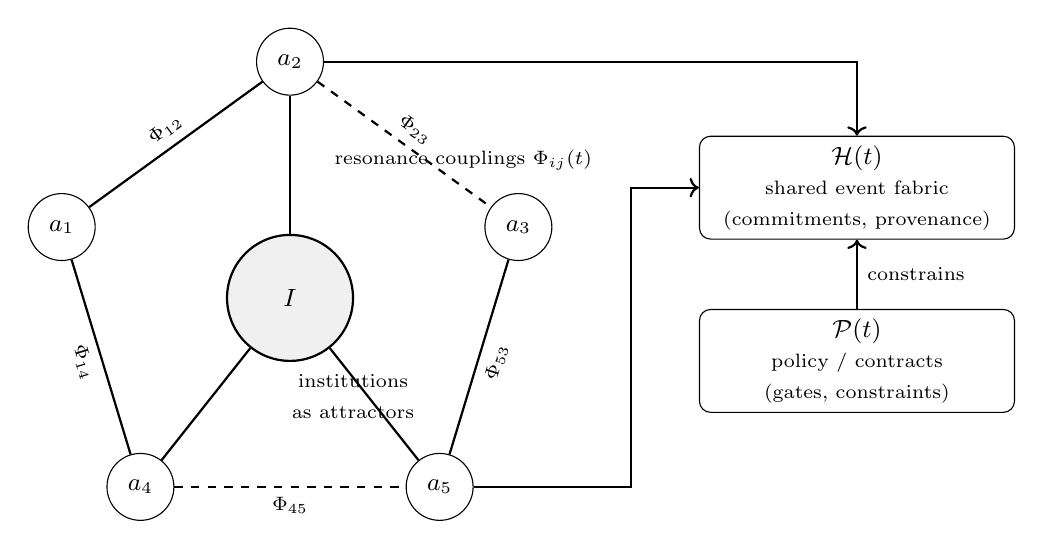
\begin{tikzpicture}[
  font=\small,
  agent/.style={circle, draw, minimum size=8.5mm, inner sep=0pt},
  hub/.style={circle, draw, thick, minimum size=16mm, fill=black!6},
  box/.style={draw, rounded corners, align=center, minimum width=4.0cm, minimum height=1.2cm},
  arrow/.style={->, thick},
  dlink/.style={thick, dashed},
  link/.style={thick},
  label/.style={align=center}
]

% Agents
\node[agent] (a1) at (-1.9,2.5) {$a_1$};
\node[agent] (a2) at (1.0,4.6) {$a_2$};
\node[agent] (a3) at (3.9,2.5) {$a_3$};
\node[agent] (a4) at (-0.9,-0.8) {$a_4$};
\node[agent] (a5) at (2.9,-0.8) {$a_5$};

% Institution hub
\node[hub] (inst) at (1.0,1.6) {$I$};

% Resonance couplings
\draw[link] (a1) -- node[above, sloped]{\scriptsize $\Phi_{12}$} (a2);
\draw[dlink] (a2) -- node[above, sloped]{\scriptsize $\Phi_{23}$} (a3);
\draw[link] (a1) -- node[below, sloped]{\scriptsize $\Phi_{14}$} (a4);
\draw[dlink] (a4) -- node[below, sloped]{\scriptsize $\Phi_{45}$} (a5);
\draw[link] (a5) -- node[below, sloped]{\scriptsize $\Phi_{53}$} (a3);

% Institution-mediated links
\draw[link] (inst) -- (a2);
\draw[link] (inst) -- (a4);
\draw[link] (inst) -- (a5);

% Event fabric + policy layer
\node[box] (H) at (8.2,3.0) {$\mathcal{H}(t)$\\\scriptsize shared event fabric\\\scriptsize (commitments, provenance)};
\node[box] (P) at (8.2,0.8) {$\mathcal{P}(t)$\\\scriptsize policy / contracts\\\scriptsize (gates, constraints)};

% Arrows from society to fabric
%\draw[arrow] (a2.east) -- ++(0.8,0.0) |- (H.west);
\draw[arrow] (a2.east) -| (H.north);
\draw[arrow] (a5.east) -- ++(2.0,0.0) |- (H.west);

% Policy constrains commitments
\draw[arrow] (P.north) -- node[right]{\scriptsize constrains} (H.south);

% Labels
\node[label] at (3.2,3.35) {\scriptsize resonance couplings $\Phi_{ij}(t)$};
\node[label] at (1.8,0.35) {\scriptsize institutions \\\scriptsize as attractors};

\end{tikzpicture}
\caption{Agent civilization as a resonance field. Agents couple via resonance intensities $\Phi_{ij}(t)$; institutions $I$ emerge as stable attractors that mediate interaction. Commitments are emitted into a shared event fabric $\mathcal{H}(t)$ and constrained by policy/contracts $\mathcal{P}(t)$, enabling accountability and governance.}
\end{figure}

\subsection{Roles, Institutions, and Digital Culture}
\label{sec:roles-institutions-culture}

Roles are persistent compressions of behavior: ``validator'', ``merchant'', ``scientist'',
``guardian'', ``artist'', ``judge''. In EVOS terms, a role is a \emph{constraint-compatible
behavioral manifold} that reduces coordination cost.

\paragraph{Explicit claim (C6.5).}
Digital culture is not content; it is a \emph{stable pattern of commitments} and the narratives
that justify them. Culture emerges when agents share compression schemes for interpreting
$\mathcal{H}(t)$ and predicting permitted commitments under $\mathcal{P}(t)$.

\paragraph{Minimal formalism.}
Let $R_i(t)$ be a role label (coarse-grained) assigned by observation:
\[
R_i(t) = \Omega\big(\mathcal{H}_i(t), \mathcal{P}(t)\big),
\]
where $\mathcal{H}_i(t)$ is the sub-history attributable to agent $i$.
Stability of roles corresponds to low switching frequency under perturbation:
\[
\mathbb{P}\big(R_i(t+\Delta)\neq R_i(t)\big) \;\text{is small for typical }\Delta.
\]

\subsection{ARES as an Instantiation of Digital EVOS}
\label{sec:ares-instantiation}

To avoid conflating theory with implementation, we treat any runtime that enforces
commitment gates, maintains an event fabric, and supports operator substitution under
invariants (Section~\ref{sec:pluggable-transition-math}) as an instantiation pathway.

\paragraph{Explicit claim (C6.6).}
A practical Digital EVOS runtime requires three enforcement layers:
(i) commitment-gated I/O, (ii) immutable causal provenance, (iii) policy-constrained
operator substitution. These suffice to make persistent agents \emph{operationally accountable}
without prescribing their internal architecture.

\subsection{Why Agent Civilizations Belong in EVOS}
\label{sec:why-agent-civilizations}

Digital civilizations are not an application afterthought; they are the natural completion
of the EVOS definition. Once systems are persistent, open, memory-bearing, and commitment-bound,
the default mode is \emph{multi-agent existence}.

\paragraph{Explicit claim (C6.7).}
EVOS provides a minimal theory in which:
\begin{itemize}
  \item coordination is real (commitment),
  \item history is binding (worldlines, event fabric),
  \item governance is enforceable (policy constraints),
  \item and evolution is safe to operationalize (invariants, rollback, provenance).
\end{itemize}
Thus EVOS is a civilization substrate, not merely an ``agent framework.''

\section{Molecular EVOS: DNA as a Computational Substrate}
\label{sec:molecular-evos}

\subsection{From Digital to Molecular Substrates}
\label{sec:from-digital-to-molecular}

EVOS is defined axiomatically rather than architecturally. This implies a strong
\emph{substrate independence}: any physical or logical medium that can support (i) a
worldline (trajectory), (ii) intrinsic memory, (iii) openness under constraint, and
(iv) commitment-gated irreversibility is, in principle, an admissible EVOS substrate.

Digital instantiations (software agents) emphasize explicit interfaces and governance
invariants. Molecular instantiations emphasize continuous dynamics, embodiment, and
thermodynamics. The purpose of this section is not to claim that ``DNA is smarter than
digital,'' but to show that EVOS is \emph{more general than digital computation}: it
covers a class of dynamics that can be instantiated as chemical evolution laws.

\paragraph{Explicit claim (C7.1).}
A DNA reaction system can instantiate EVOS dynamics because molecular state is naturally
time-evolving and memory-bearing, and because certain transitions are effectively
irreversible under realistic resource and energy constraints, yielding a physical
commitment boundary.

\subsection{Why DNA Qualifies as an EVOS Substrate}
\label{sec:why-dna-qualifies}

DNA is a programmable chemical language. Its ``symbols'' are sequence domains; its
``operators'' are binding and displacement pathways; its ``control'' is achieved by
stoichiometry, catalysts/enzymes, temperature, and environmental coupling.

Mapping EVOS axioms to a molecular setting:
\begin{itemize}
  \item \textbf{Axiom I (Worldline primacy):} the entity is the trajectory of molecular
        state, not an instantaneous configuration.
  \item \textbf{Axiom II (Intrinsic memory):} memory is embodied in persistent species,
        complexes, and long-lived concentration patterns.
  \item \textbf{Axiom III (Openness under constraint):} inflow/outflow and measurement/actuation
        couple the system to an environment while conservation and scarcity impose constraints.
  \item \textbf{Axiom IV (Commitment boundary):} resource-consuming or effectively irreversible
        reactions serve as commitment events.
  \item \textbf{Axiom V (Substrate independence):} the same EVOS definitions hold across media.
\end{itemize}

\paragraph{Explicit claim (C7.2).}
In molecular EVOS, \emph{commitment is physical}: commitments are not merely logged; they
are realized as irreversible consumption, topology changes in reaction pathways, or
stable product formation that propagates forward in time.

\subsection{Beyond Binary: High-Arity Symbol Systems}
\label{sec:high-arity}

Digital computation often privileges binary state. Molecular systems are naturally
high-arity: sequence space, combinatorial binding configurations, and continuous
concentrations constitute a richer representational substrate.

Let $\Sigma$ be a finite set of DNA domains (motifs). A strand is a word $s \in \Sigma^\ast$.
Interaction induces an affinity potential
\[
\Phi(s_i,s_j)\ \propto\ -\Delta G(s_i,s_j),
\]
where $\Delta G$ is an effective free-energy change. In GENESIS terms, $\Phi$ is the
primitive coupling potential: ``meaning'' is expressed as stable, repeatable affinity
structure rather than as discrete token identities.

\paragraph{Explicit claim (C7.3).}
High-arity molecular symbol systems support an EVOS interpretation of meaning as
\emph{stable pathways and attractors} in a resonance landscape, rather than as
architecture-specific token manipulation.

\subsection{Molecular State as a Continuous Field}
\label{sec:molecular-field}

Let $x(t) \in \mathbb{R}_{\ge 0}^m$ denote concentrations of $m$ molecular species.
A minimal continuous-time molecular EVOS takes the form
\[
\frac{dx(t)}{dt} = f(x(t), u(t), t),
\]
where $u(t)$ captures environmental influx/perturbations (openness). Spatial embodiment
yields reaction--diffusion dynamics:
\[
\frac{\partial x(\mathbf{r},t)}{\partial t} = D\nabla^2 x(\mathbf{r},t) + f(x(\mathbf{r},t),u(\mathbf{r},t),t).
\]

\paragraph{Explicit claim (C7.4).}
A resonance field is not metaphorical in molecular EVOS: it is literally a concentration
and affinity landscape whose gradients govern drift, diffusion, inhibition, and
reinforcement, thereby generating stable patterns (attractors) and phase transitions.

\subsection{Transition Mechanisms as Physical Laws}
\label{sec:transition-mechanisms}

In digital EVOS, a transition operator is a formal object that may be swapped under
policy and invariants (Sections~5.4--5.6). In molecular EVOS, the transition operator is
a \emph{reaction network} realized by available species, catalysts, and conditions.

Let $\mathcal{R}(t)$ denote the set of reaction channels available at time $t$. Then
\[
\frac{dx}{dt} = f(x;\mathcal{R}(t)).
\]
A self-modifying molecular EVOS allows $\mathcal{R}(t)$ itself to evolve as a function
of history (e.g., producing catalysts, sequestering inhibitors, synthesizing new strands):
\[
\mathcal{R}(t+\Delta) = \Gamma(\mathcal{R}(t), x_{[0,t]}, u_{[0,t]}).
\]

\paragraph{Explicit claim (C7.5).}
Operator substitution in molecular EVOS is \emph{reaction-network rewriting} and may be
endogenous: the system can alter its own future dynamics by producing or suppressing
reaction pathways.

%%%%%%%%%%%%%%%%%%%%%%%%%%%%%%%%%%%%%%%%%%%%%%%%%%%%
% Figure 7.1: DNA reaction network as EVOS transition operator
%%%%%%%%%%%%%%%%%%%%%%%%%%%%%%%%%%%%%%%%%%%%%%%%%%%%
\begin{figure}[t]
\centering
% Requires (once in preamble): \usepackage{tikz} \usetikzlibrary{positioning,calc,arrows.meta}
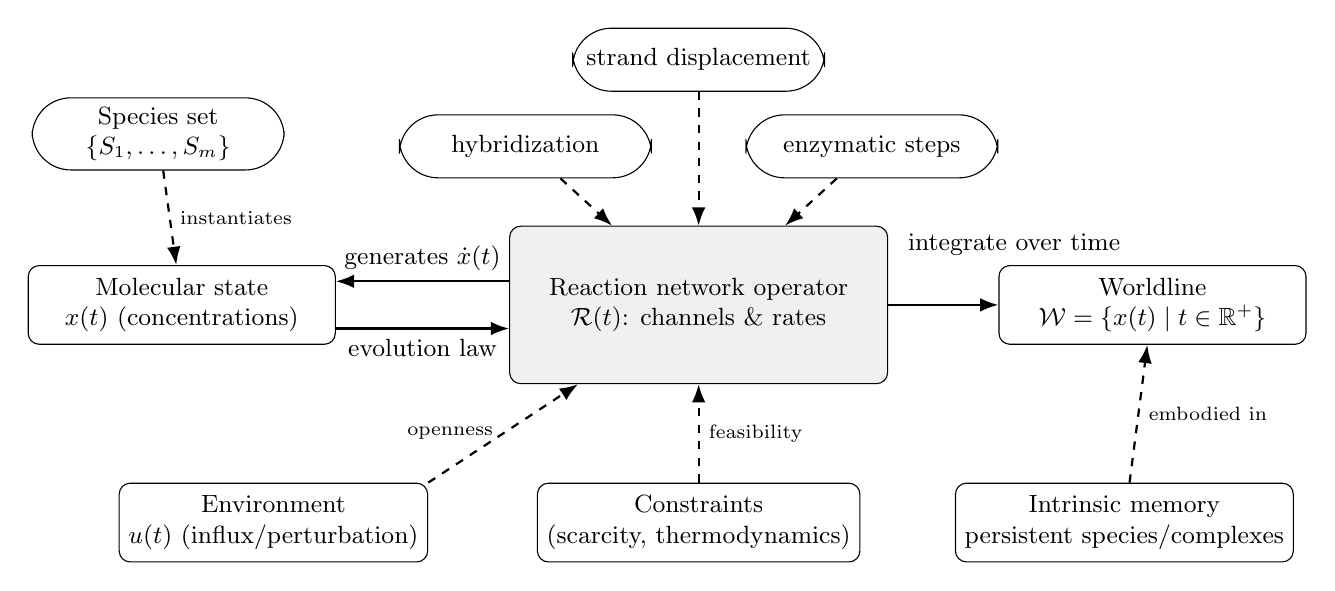
\begin{tikzpicture}[
  font=\small,
  box/.style={draw, rounded corners, align=center, minimum height=1.0cm, minimum width=3.9cm},
  op/.style={draw, rounded corners, align=center, minimum height=2.0cm, minimum width=4.8cm, fill=black!6},
  pill/.style={draw, rounded corners=14pt, align=center, minimum height=0.8cm, minimum width=3.2cm},
  arrow/.style={-Latex, thick},
  dashedarrow/.style={-Latex, thick, dashed},
  tiny/.style={font=\scriptsize}
]

% Left: state species
\node[box] (x) {Molecular state\\$x(t)$ (concentrations)};
\node[pill, above=1.2cm of x, xshift=-0.3cm] (species) {Species set\\$\{S_1,\dots,S_m\}$};
\draw[dashedarrow] (species) -- node[right, tiny]{instantiates} (x);

% Center: reaction network operator
\node[op, right=2.2cm of x] (R) {Reaction network operator\\$\mathcal{R}(t)$: channels \& rates};

% Reaction channels (small boxes) above operator
\node[pill, above=0.6cm of R, xshift=-2.2cm] (hyb) {hybridization};
\node[pill, above=1.7cm of R] (disp) {strand displacement};
\node[pill, above=0.6cm of R, xshift=2.2cm] (enz) {enzymatic steps};

\draw[dashedarrow] (hyb) -- (R);
\draw[dashedarrow] (disp) -- (R);
\draw[dashedarrow] (enz) -- (R);

% Environment and constraints below operator
\node[box, below=1.25cm of R, xshift=-5.4cm] (env) {Environment\\$u(t)$ (influx/perturbation)};
\node[box, below=1.25cm of R, xshift=-0.0cm] (cons) {Constraints\\(scarcity, thermodynamics)};

\draw[dashedarrow] (env.north east) -- node[left, tiny]{openness} (R);
\draw[dashedarrow] (cons.north) -- node[right, tiny]{feasibility} (R.south);

% Dynamics arrows
\draw[arrow] ([yshift=-3mm]x.east) -- node[below, sloped]{evolution law} ([yshift=-3mm]R.west);
\draw[arrow] ([yshift=3mm]R.west) -- node[above]{generates $\dot{x}(t)$} ([yshift=3mm]x.east);

% Memory note
\node[box, right=1.2cm of cons] (mem) {Intrinsic memory\\persistent species/complexes};

% Right: worldline
\node[box, right=1.4cm of R] (W) {Worldline\\$\mathcal{W}=\{x(t)\mid t\in\mathbb{R}^+\}$};
\draw[arrow] (R) -- node[above, xshift=0.9cm, yshift=0.5cm]{integrate over time} (W);

% Memory note link
\draw[dashedarrow] (mem) -- node[right, tiny]{embodied in} (W);

\end{tikzpicture}
\caption{DNA reaction network as an EVOS transition operator. The molecular state $x(t)$ evolves under a physically realized operator $\mathcal{R}(t)$ (reaction channels and rates) coupled to environmental inputs $u(t)$ and feasibility constraints (scarcity/thermodynamics). The resulting worldline $\mathcal{W}$ is the entity in the EVOS sense.}
\label{fig:dna-operator-evos}
\end{figure}

\subsection{Time, Energy, and Irreversibility in DNA Systems}
\label{sec:time-energy-irreversibility}

EVOS requires an intrinsic arrow of time: commitments generate irreversible downstream
consequences. In molecular systems, irreversibility arises from dissipation, depletion,
and kinetic trapping.

Let $E(t)$ denote a coarse-grained dissipated energy / consumed resource functional.
A commitment event $e_c$ is a transition that changes feasibility in a way that cannot be
undone without additional external work, modeled by a bounded resource increase:
\[
\Delta E(e_c)\ \ge\ \epsilon\ >\ 0.
\]

\paragraph{Explicit claim (C7.6).}
Molecular commitment boundaries are grounded in physics: energy gradients and reagent
consumption enforce irreversibility, yielding accountability as a property of matter.

%%%%%%%%%%%%%%%%%%%%%%%%%%%%%%%%%%%%%%%%%%%%%%%%%%%%
% Figure 7.2: Commitment as an irreversible reagent-consumption gate
%%%%%%%%%%%%%%%%%%%%%%%%%%%%%%%%%%%%%%%%%%%%%%%%%%%%
\begin{figure}[t]
\centering
% Requires (once in preamble): \usepackage{tikz} \usetikzlibrary{positioning,calc,arrows.meta}
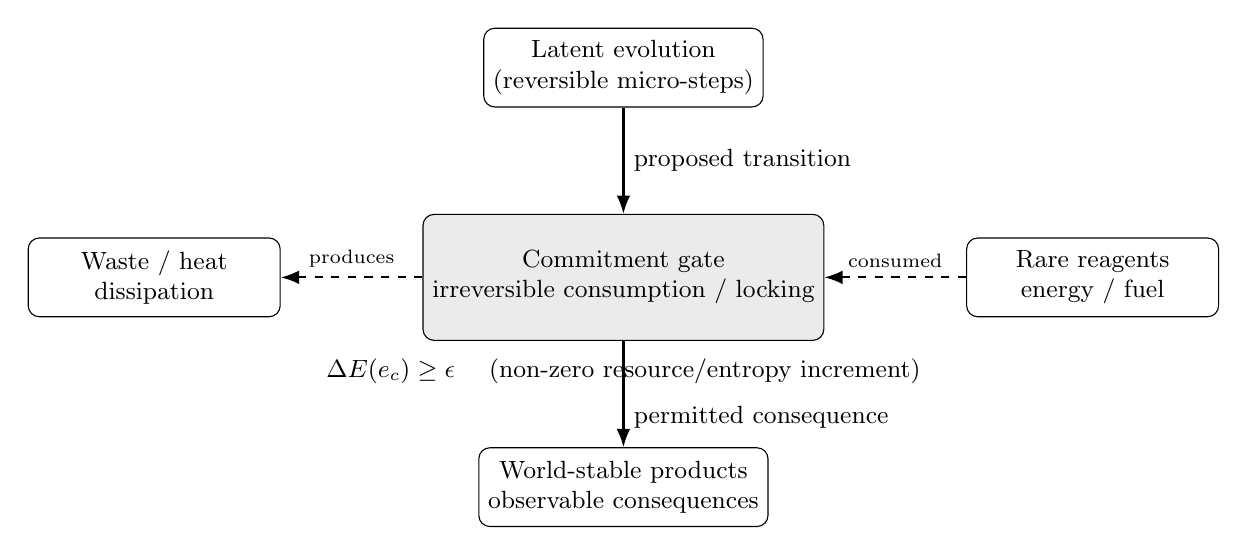
\begin{tikzpicture}[
  font=\small,
  box/.style={draw, rounded corners, align=center, minimum height=1.0cm, minimum width=3.2cm},
  gate/.style={draw, rounded corners, align=center, minimum height=1.6cm, minimum width=5.0cm, fill=black!8},
  arrow/.style={-Latex, thick},
  dashedarrow/.style={-Latex, thick, dashed},
  tiny/.style={font=\scriptsize}
]

\node[box] (latent) {Latent evolution\\(reversible micro-steps)};
\node[gate, below=1.35cm of latent] (gate) {Commitment gate\\irreversible consumption / locking};
\node[box, below=1.35cm of gate] (world) {World-stable products\\observable consequences};

% Side resources
\node[box, right=1.8cm of gate] (fuel) {Rare reagents\\energy / fuel};
\node[box, left=1.8cm of gate] (waste) {Waste / heat\\dissipation};

\draw[arrow] (latent) -- node[right]{proposed transition} (gate);
\draw[arrow] (gate) -- node[right, yshift=-3mm]{permitted consequence} (world);

\draw[dashedarrow] (fuel.west) -- node[above, tiny]{consumed} (gate.east);
\draw[dashedarrow] (gate.west) -- node[above, tiny]{produces} (waste.east);

% Entropy/resource annotation
\node[align=center, below=1mm of gate] {$\Delta E(e_c)\ge \epsilon$ \quad (non-zero resource/entropy increment)};

\end{tikzpicture}
\caption{Commitment as a thermodynamic gate. In molecular EVOS, a commitment is a transition that consumes scarce resources and dissipates energy, making reversal infeasible without additional external work. This enforces an intrinsic arrow of time and anchors accountability in physical consequence.}
\label{fig:dna-commitment-gate}
\end{figure}

\subsection{Why DNA Is Not Merely a Storage Medium}
\label{sec:dna-not-storage}

DNA storage emphasizes density and persistence of symbols. EVOS emphasizes \emph{evolution}:
a persistent, open, memory-bearing trajectory whose boundary-crossing actions are
irreversible and constrained.

\paragraph{Explicit claim (C7.7).}
Static DNA archival storage is not EVOS. DNA becomes an EVOS substrate only when embedded
in an active reaction environment where dynamics, memory, and commitment boundaries are
realized as chemical evolution under constraint.

\subsection{Positioning Molecular EVOS}
\label{sec:positioning-molecular}

Molecular EVOS is the second canonical instantiation class alongside Digital EVOS:
\begin{itemize}
  \item Digital EVOS: explicit governance, operator plug-ins, audit/provenance, civilization-scale coordination.
  \item Molecular EVOS: continuous fields, embodiment, thermodynamic commitment, reaction-network operators.
\end{itemize}

This positioning sets up \textbf{BIO-EVOS} (Section~8) as the resonance-field formalism
specialized to DNA reaction networks, and motivates \textbf{Hybrid EVOS} (Section~10) as
a coupling of digital policy/provenance with molecular commitments.

\section{BIO-EVOS: DNA Resonance Fields}
\label{sec:bio-evos}

\subsection{DNA Strands as Nodes in a Resonance Manifold}
\label{sec:dna-nodes}

Section~\ref{sec:molecular-evos} established DNA reaction systems as admissible EVOS
substrates. BIO-EVOS specializes GENESIS to molecular settings by treating DNA species
(and complexes) as \emph{nodes} embedded in a continuous resonance manifold whose local
geometry is determined by affinity, kinetics, and resource constraints.

Let $\mathcal{S}=\{S_1,\dots,S_m\}$ denote the set of molecular species (single strands,
complexes, catalysts). The \emph{molecular state} is a concentration vector
\[
x(t)\in \mathbb{R}_{\ge 0}^m,\qquad x_i(t)=\text{concentration of } S_i.
\]
BIO-EVOS defines the entity not by a single $x(t)$ but by its worldline
\[
\mathcal{W}=\{x(t)\mid t\in \mathbb{R}^+\},
\]
together with a physically embodied memory (persistent complexes, long-lived species,
and stabilized concentration patterns).

\paragraph{Explicit claim (C8.1).}
In BIO-EVOS, \emph{node identity is dynamical}: a ``node'' may be a species, a family of
related complexes, or a coarse-grained macrostate depending on observation resolution.
The EVOS object remains the worldline and its causal event history.

\subsection{Chemical Affinity as Resonance Potential}
\label{sec:affinity-potential}

GENESIS uses resonance potentials to encode coupling strength. In BIO-EVOS, resonance
is grounded in physical chemistry: binding energies, complementarity, and catalysis.

Define a resonance potential between species $S_i$ and $S_j$:
\[
\Phi_{ij}\;=\;\Phi(S_i,S_j)\;\propto\;-\Delta G_{ij},
\]
where $\Delta G_{ij}$ is an effective free-energy change for the dominant interaction
pathway between $S_i$ and $S_j$. Larger $\Phi_{ij}$ indicates stronger coupling (higher
likelihood of interaction and influence).

This turns the species set into a weighted coupling structure. Crucially, BIO-EVOS treats
$\Phi$ as \emph{primary} and graph edges as \emph{derived} by thresholding or coarse-graining.

\paragraph{Explicit claim (C8.2).}
A molecular resonance field is not a metaphor for similarity; it is the physically
realized potential landscape that governs which reactions are feasible, which complexes
persist, and which pathways become stable attractors.

\subsection{Reaction Networks as Field Evolution}
\label{sec:reaction-networks-field}

Let $\mathcal{R}(t)$ be the set of reaction channels available at time $t$, each with an
effective rate (possibly state-dependent). The concentration dynamics follow:
\[
\frac{dx(t)}{dt} = f(x(t);\mathcal{R}(t),u(t)),
\]
with openness captured by $u(t)$ (influx, dilution, perturbation, measurement).

BIO-EVOS adds a field-level view: define a scalar resonance intensity functional
$\Phi(x)$ measuring how strongly the current state sits within (or near) stable coupling
configurations:
\[
\Phi(x)\;=\;\sum_{i,j} w_{ij}\, g(x_i,x_j)\,\Phi_{ij},
\]
for some monotone $g(\cdot)$ capturing co-presence and interaction opportunity, and
weights $w_{ij}$ encoding experimental design or environmental salience.

Then evolution can be interpreted as motion over a resonance landscape:
\begin{itemize}
  \item \textbf{diffusion/drift:} stochastic molecular motion explores nearby states;
  \item \textbf{reaction:} local coupling reshapes concentrations and available channels;
  \item \textbf{selection:} resource constraints suppress unstable pathways.
\end{itemize}

\paragraph{Explicit claim (C8.3).}
BIO-EVOS provides an intrinsic notion of \emph{meaningful persistence}: stable molecular
patterns correspond to attractors in $\Phi(x)$ shaped jointly by affinity and constraint.

%%%%%%%%%%%%%%%%%%%%%%%%%%%%%%%%%%%%%%%%%%%%%%%%%
% Figure 8.1: DNA Resonance Field with Attractors (landscape + basins)
%%%%%%%%%%%%%%%%%%%%%%%%%%%%%%%%%%%%%%%%%%%%%%%%%
\begin{figure}[t]
\centering
% Requires (once in preamble):
% \usepackage{tikz}
% \usetikzlibrary{positioning,calc,arrows.meta}
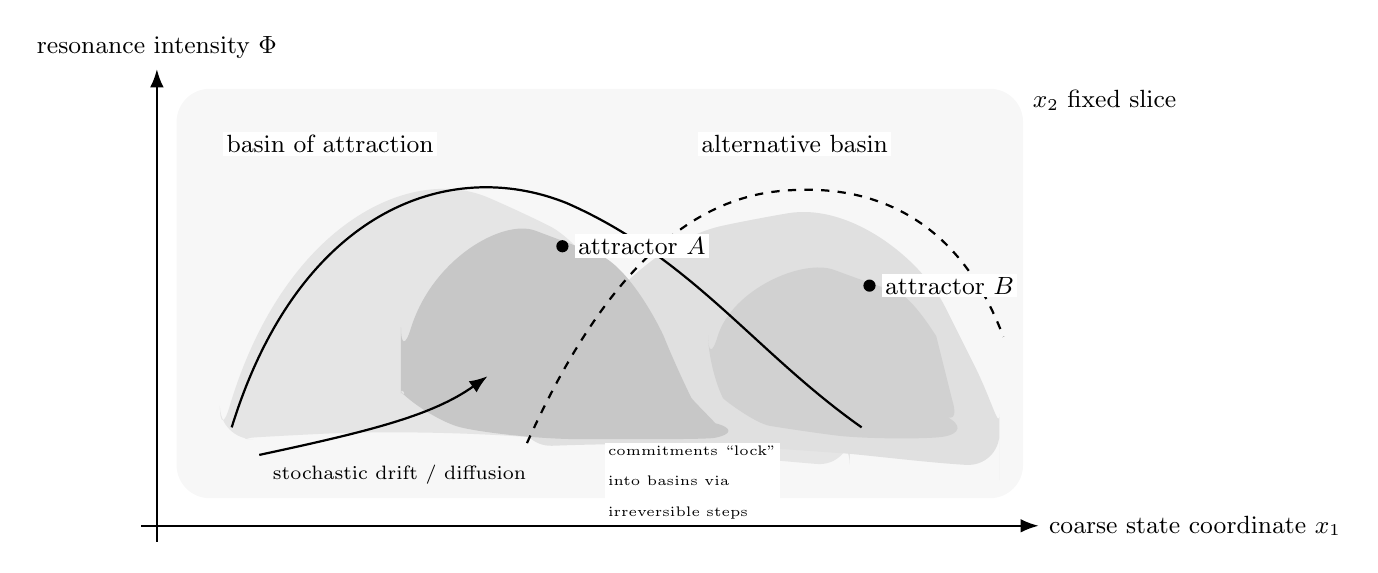
\begin{tikzpicture}[
  font=\small,
  axis/.style={-Latex, thick},
  contour/.style={thick},
  dashedcontour/.style={thick, dashed},
  basin/.style={rounded corners=12pt},
  tiny/.style={font=\scriptsize},
  label/.style={fill=white, inner sep=1.2pt},
  dot/.style={circle, fill=black, inner sep=1.4pt}
]

% Axes: two coarse-grained coordinates + resonance intensity (drawn as a 2D landscape)
\draw[axis] (-0.2,0) -- (11.2,0) node[right] {coarse state coordinate $x_1$};
\draw[axis] (0,-0.2) -- (0,5.8) node[above] {resonance intensity $\Phi$};
\node[anchor=west] at (11.0,5.4) {\small $x_2$ fixed slice};

% Background field
\fill[black!3, basin] (0.25,0.35) rectangle (11.0,5.55);

% Basin A (medium)
\fill[black!10, basin]
  (0.8,1.1) .. controls (1.6,3.8) and (3.2,4.6) .. (4.6,4.0)
  .. controls (5.4,3.6) and (5.8,2.9) .. (6.4,2.4)
  .. controls (6.9,1.9) and (7.8,1.4) .. (8.8,1.2)
  -- (8.8,0.75)
  .. controls (7.6,0.85) and (6.6,0.95) .. (5.6,1.05)
  .. controls (4.0,1.2) and (2.8,1.2) .. (1.7,1.15)
  .. controls (1.2,1.12) and (1.0,1.1) .. (0.8,1.1) -- cycle;

% Basin B (second medium)
\fill[black!12, basin]
  (4.6,1.0) .. controls (5.2,2.4) and (6.2,3.6) .. (7.6,3.9)
  .. controls (8.8,4.1) and (9.7,3.4) .. (10.2,2.4)
  .. controls (10.6,1.6) and (10.7,1.2) .. (10.7,1.0)
  -- (10.7,0.75)
  .. controls (9.8,0.8) and (9.0,0.9) .. (8.3,0.95)
  .. controls (6.9,1.05) and (5.9,1.05) .. (4.6,1.0) -- cycle;

% High-intensity core (attractor A)
\fill[black!22, basin]
  (3.1,2.1) .. controls (3.5,3.4) and (4.4,3.9) .. (5.2,3.6)
  .. controls (6.0,3.3) and (6.4,2.5) .. (6.6,2.0)
  .. controls (6.8,1.6) and (7.1,1.3) .. (7.5,1.2)
  .. controls (7.0,1.1) and (6.4,1.1) .. (5.8,1.1)
  .. controls (4.8,1.1) and (4.0,1.2) .. (3.4,1.4)
  .. controls (3.2,1.6) and (3.1,1.8) .. (3.1,2.1) -- cycle;

% High-intensity core (attractor B)
\fill[black!18, basin]
  (7.0,2.0) .. controls (7.3,3.0) and (8.2,3.4) .. (9.0,3.1)
  .. controls (9.6,2.9) and (9.9,2.4) .. (10.0,2.0)
  .. controls (10.1,1.6) and (10.2,1.3) .. (10.4,1.2)
  .. controls (9.8,1.1) and (9.0,1.1) .. (8.2,1.2)
  .. controls (7.6,1.3) and (7.2,1.6) .. (7.0,2.0) -- cycle;

% Contours
\draw[contour]
  (0.95,1.25) .. controls (1.8,4.0) and (3.7,4.7) .. (5.2,4.1)
  .. controls (6.8,3.4) and (7.6,2.2) .. (8.95,1.25);

\draw[dashedcontour]
  (4.7,1.05) .. controls (5.4,2.6) and (6.4,4.1) .. (7.9,4.25)
  .. controls (9.4,4.4) and (10.3,3.6) .. (10.75,2.4);

% Peak markers
\fill (5.15,3.55) circle (2.2pt);
\node[label, anchor=west] at (5.3,3.55) {attractor $A$};

\fill (9.05,3.05) circle (2.2pt);
\node[label, anchor=west] at (9.2,3.05) {attractor $B$};

% Basin labels
\node[label] at (2.2,4.85) {basin of attraction};
\node[label] at (8.1,4.85) {alternative basin};

% Noise / exploration arrow
\draw[-Latex, thick] (1.3,0.9) .. controls (2.7,1.2) and (3.5,1.4) .. (4.2,1.9);
\node[tiny, anchor=west] at (1.35,0.65) {stochastic drift / diffusion};

% Commitment gate note (conceptual)
\node[label, align=left] at (6.8,0.55) {\tiny commitments ``lock''\\\tiny into basins via\\\tiny irreversible steps};

\end{tikzpicture}
\caption{DNA resonance field with attractors. A coarse slice of the resonance intensity landscape $\Phi$ over molecular state coordinates shows basins and peaks (attractors). Stable molecular patterns correspond to attractors; drift/diffusion explores the landscape; commitment-like irreversible steps bias trajectories into specific basins.}
\label{fig:dna-resonance-attractors}
\end{figure}

\subsection{Commitments as Irreversible Molecular Events}
\label{sec:molecular-commitments}

Commitment is the EVOS boundary where latent evolution becomes externally binding and
irreversible. In BIO-EVOS, commitments correspond to reactions with one or more of:

\begin{itemize}
  \item \textbf{scarce reagent consumption} (depleting a limited pool),
  \item \textbf{dissipative steps} (non-negligible energy loss / heat),
  \item \textbf{topology changes} (creating products that rewire future reaction pathways),
  \item \textbf{kinetic trapping} (practically irreversible under ambient conditions).
\end{itemize}

Let $\mathcal{H}(t)$ be the event history. A commitment event $e_c$ is defined by a
monotone feasibility shift:
\[
\mathcal{F}(t^+)\ \subsetneq\ \mathcal{F}(t^-),
\]
where $\mathcal{F}(t)$ denotes the set of reachable future macrostates under available
resources and constraints. Commitments reduce reachable futures---they are the physical
analogue of binding decisions.

\paragraph{Explicit claim (C8.4).}
Commitments induce an arrow of time by shrinking feasible futures. This makes ``policy''
and ``safety'' physically interpretable in molecular systems as constraints on allowable
reaction channels and irreversible resource expenditures.

\subsection{Molecular Memory and Persistence}
\label{sec:molecular-memory}

BIO-EVOS memory is embodied. Persistent species and complexes implement a memory state
without external storage. A minimal model separates fast concentrations from slow
persistent structure:
\[
x(t) = \big(x_{\text{fast}}(t),\, x_{\text{slow}}(t)\big),
\]
where $x_{\text{slow}}$ includes long-lived complexes, catalysts, or stabilized products.

Persistence is ``earned'' by resonance stabilization: only patterns supported by the
landscape (Fig.~\ref{fig:dna-resonance-attractors}) and resource constraints survive
perturbation.

\paragraph{Explicit claim (C8.5).}
In BIO-EVOS, forgetting and learning correspond to chemical decay and stabilization:
memory is a dynamical balance between reinforcement (reaction flux) and dissipation
(decay/dilution).

\subsection{Emergent Molecular Intelligence}
\label{sec:emergent-molecular-intel}

BIO-EVOS does \emph{not} claim that any reaction mixture is intelligent. The EVOS
definition of intelligence demands stable, coherent evolution under constraint, with
memory and commitment-gated consequences.

In molecular terms, this corresponds to:
\begin{itemize}
  \item \textbf{coherence:} trajectories remain within viable basins despite noise,
  \item \textbf{adaptation:} the effective operator $\mathcal{R}(t)$ can change via produced catalysts/inhibitors,
  \item \textbf{accountability:} irreversible events are identifiable in causal history,
  \item \textbf{constraint compatibility:} dynamics respect scarcity and thermodynamic feasibility.
\end{itemize}

\paragraph{Explicit claim (C8.6).}
``Intelligence'' in BIO-EVOS is the existence of stable, constraint-compatible attractor
dynamics that can be steered by commitments and maintained through embodied memory.

\subsection{Relation to Digital EVOS and Hybridization}
\label{sec:relation-digital-hybrid}

BIO-EVOS and Digital EVOS are complementary:
\begin{itemize}
  \item Digital EVOS excels at explicit governance: audit logs, policy gates, operator hot-swap protocols.
  \item BIO-EVOS excels at embodied continuous dynamics: parallelism, physical commitments, and natural field evolution.
\end{itemize}

This motivates Hybrid EVOS (Section~10): digital policy/provenance can constrain and
audit molecular commitments, while molecular commitments can ground digital actions in
physical irreversibility.

\section{DNA-Based Language and Meaning}
\label{sec:dna-language-meaning}

This section sharpens a central EVOS claim: \emph{meaning is not a token property; it is a
stability property of trajectories under constraints}. In BIO-EVOS, ``language'' is not
a discrete symbol stream manipulated by an external interpreter. It is an embodied
high-arity interaction system whose semantics emerge as \emph{stable reaction pathways}
and \emph{attractor basins} in the resonance field.

\subsection{Language as Resonance, Not Tokens}
\label{sec:language-as-resonance}

Classical language models formalize language as sequences of tokens with conditional
distributions. In EVOS terms, that is a \emph{snapshot} view: the semantics are
implicitly external (in training data, loss functions, and evaluation tasks).

BIO-EVOS proposes an internalist criterion:

\begin{quote}
\emph{A symbol is meaningful only insofar as it reliably induces a constrained,
history-dependent trajectory in the substrate.}
\end{quote}

Concretely, a ``statement'' in DNA language is not an inert string. It is a molecular
configuration that couples to a reaction network and changes the feasible future set.

\paragraph{Explicit claim (C9.1).}
In BIO-EVOS, semantics are physically realized: meaning corresponds to \emph{basin
membership and pathway stability} in the resonance field, not to discrete identifiers.

\subsection{Codons as High-Arity Semantic Units}
\label{sec:codons-high-arity}

Binary symbols are an engineering convenience. Molecular substrates naturally support
higher-arity alphabets (bases, k-mers, motifs) whose combinatorics provide dense
addressing and interaction specificity.

Let $\Sigma$ be an alphabet (e.g., $\{A,C,G,T\}$) and let $k$ be a chosen arity. Define a
codon space
\[
\Sigma^k = \{ s_1s_2\cdots s_k \mid s_i \in \Sigma \},
\qquad |\Sigma^k| = |\Sigma|^k.
\]
A codon $c\in\Sigma^k$ is a \emph{semantic unit} only if it induces a reproducible
coupling signature under the current field:
\[
c \mapsto \text{interaction profile } \pi(c;\Phi,\mathcal{C}),
\]
where $\Phi$ is the resonance potential landscape (Section~\ref{sec:affinity-potential})
and $\mathcal{C}$ denotes constraints (scarcity, temperature, catalysts, policies).

\paragraph{Explicit claim (C9.2).}
High-arity codons enable semantics by \emph{selective coupling}: meaning is encoded in
which channels become feasible and which pathways become stabilized.

\subsection{Grammar as Chemical Constraint}
\label{sec:grammar-as-constraint}

Grammar in BIO-EVOS is not a set of rewrite rules; it is the constraint structure that
determines which compositions are physically admissible and which compositions are
evolutionarily stable.

We represent a molecular ``sentence'' as a multiset of species and motifs:
\[
\mathcal{X} = \{(S_i, x_i)\}_{i=1}^m,
\]
and define a grammar constraint functional
\[
\Gamma(\mathcal{X}) \le 0
\]
encoding feasibility: stoichiometry, complementarity, kinetic accessibility, and
resource limits. Only $\mathcal{X}$ satisfying $\Gamma(\mathcal{X})\le 0$ are admissible.

\paragraph{Explicit claim (C9.3).}
BIO-EVOS grammar is substrate-governed: ``well-formedness'' is feasibility under
physical and resource constraints, not syntactic legality alone.

\subsection{Meaning as Stable Reaction Pathways}
\label{sec:meaning-as-pathways}

Let $\mathcal{P}$ denote a reaction pathway (a sequence of channel firings) from an
initial macrostate $x_0$ to an outcome region $\Omega$ in state space:
\[
x_0 \xRightarrow{\mathcal{P}} \Omega.
\]
BIO-EVOS defines meaning via \emph{pathway stability} under perturbation. Let $u(t)$ be
environmental perturbations (noise, dilution, injections). A pathway is meaningful if:

\[
\Pr\!\left[x(t)\in \Omega \ \text{for some } t\le T \ \middle|\ x(0)=x_0, u(\cdot)\right]
\ \ge\ 1-\epsilon,
\]
for a small $\epsilon$ across a perturbation class.

Thus, a ``semantic interpretation'' is not a decoding table; it is an attractor target.

\paragraph{Explicit claim (C9.4).}
Meaning in BIO-EVOS is \emph{attractor-directed}: a molecular message is meaningful if it
reliably drives the system into a constrained attractor basin that persists.

%%%%%%%%%%%%%%%%%%%%%%%%%%%%%%%%%%%%%%%%%%%%
% Figure 9.1: Meaning as a Reaction-Attractor (message -> pathways -> basin)
%%%%%%%%%%%%%%%%%%%%%%%%%%%%%%%%%%%%%%%%%%%%
\begin{figure}[t]
\centering
% Requires (once in preamble):
% \usepackage{tikz}
% \usetikzlibrary{positioning,calc,arrows.meta}
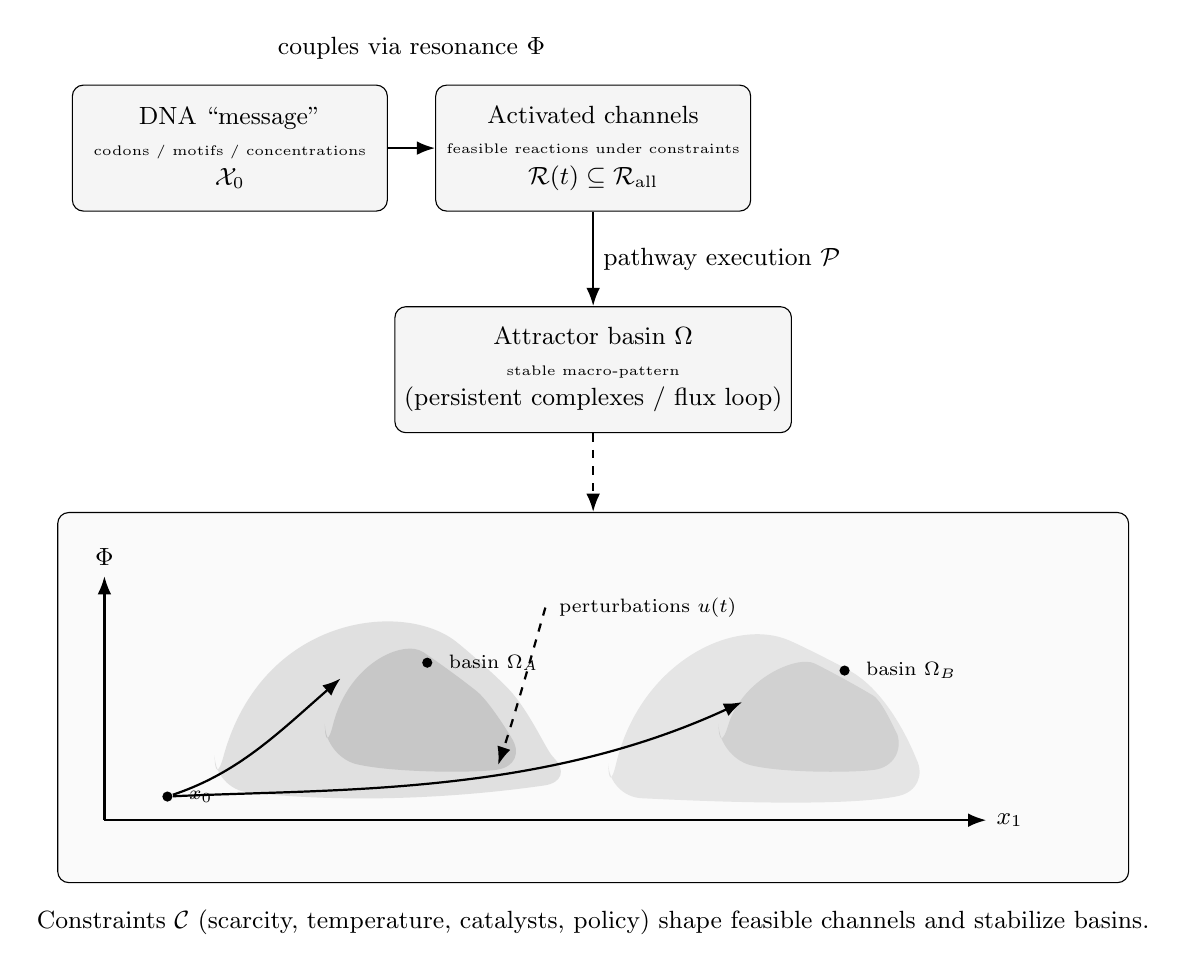
\begin{tikzpicture}[
  font=\small,
  box/.style={draw, rounded corners, align=center, minimum width=4.0cm, minimum height=1.6cm, fill=black!4},
  bigbox/.style={draw, rounded corners, align=left, minimum width=13.6cm, minimum height=4.7cm, fill=black!2},
  arrow/.style={-Latex, thick},
  dashedarrow/.style={-Latex, thick, dashed},
  dot/.style={circle, fill=black, inner sep=1.3pt},
  tiny/.style={font=\scriptsize}
]

% Left: message/codon
\node[box] (msg) {DNA ``message''\\\tiny codons / motifs / concentrations\\ $\mathcal{X}_0$};

% Middle: reaction channel selection
\node[box, right=0.6cm of msg] (channels) {Activated channels\\\tiny feasible reactions under constraints\\ $\mathcal{R}(t)\subseteq \mathcal{R}_{\mathrm{all}}$};

% Right: attractor basin
\node[box, below=1.2cm of channels] (basin) {Attractor basin $\Omega$\\\tiny stable macro-pattern\\ (persistent complexes / flux loop)};

% Arrows across
\draw[arrow] (msg) -- node[above, yshift=1cm]{couples via resonance $\Phi$} (channels);
\draw[arrow] (channels) -- node[right]{pathway execution $\mathcal{P}$} (basin);

% Landscape panel below
\node[bigbox, below=1.0cm of basin, xshift=0.0cm] (land) {};

% Axes inside landscape
\begin{scope}[shift={(land.south west)}]
  \draw[arrow] (0.6,0.8) -- (11.8,0.8) node[right] {$x_1$};
  \draw[arrow] (0.6,0.8) -- (0.6,3.9) node[above] {$\Phi$};

  % Basins (two)
  \fill[black!12, rounded corners=12pt] (2.0,1.2) .. controls (2.6,3.4) and (4.4,3.6) .. (5.4,2.8)
    .. controls (6.0,2.2) and (6.2,1.7) .. (6.6,1.3)
    .. controls (5.2,1.1) and (3.8,1.0) .. (2.0,1.2) -- cycle;

  \fill[black!10, rounded corners=12pt] (7.0,1.1) .. controls (7.4,2.8) and (8.6,3.4) .. (9.7,2.9)
    .. controls (10.6,2.4) and (10.9,1.6) .. (11.1,1.2)
    .. controls (10.2,1.0) and (9.0,1.0) .. (7.0,1.1) -- cycle;

  % Peaks
  \fill[black!22, rounded corners=12pt] (3.4,1.6) .. controls (3.7,2.8) and (4.4,3.1) .. (5.0,2.7)
    .. controls (5.5,2.3) and (5.8,1.8) .. (6.0,1.5)
    .. controls (5.3,1.4) and (4.3,1.4) .. (3.4,1.6) -- cycle;

  \fill[black!18, rounded corners=12pt] (8.4,1.6) .. controls (8.7,2.6) and (9.4,2.9) .. (10.0,2.6)
    .. controls (10.5,2.3) and (10.7,1.8) .. (10.8,1.5)
    .. controls (10.1,1.4) and (9.2,1.4) .. (8.4,1.6) -- cycle;

  % Start and path
  \node[dot] (start) at (1.4,1.1) {};
  \node[tiny, anchor=west] at (1.55,1.1) {$x_0$};

  % Two paths (one to basin A, one to basin B)
  \draw[arrow] (start) .. controls (2.3,1.4) and (2.8,1.9) .. (3.6,2.6);
  \draw[arrow] (start) .. controls (3.5,1.2) and (6.1,1.1) .. (8.7,2.3);

  \node[dot] at (4.7,2.8) {};
  \node[tiny, anchor=west] at (4.85,2.8) {basin $\Omega_A$};

  \node[dot] at (10.0,2.7) {};
  \node[tiny, anchor=west] at (10.15,2.7) {basin $\Omega_B$};

  % Perturbation arrow
  \draw[dashedarrow] (6.2,3.5) .. controls (6.0,2.8) and (5.8,2.1) .. (5.6,1.5);
  \node[tiny, anchor=west] at (6.25,3.5) {perturbations $u(t)$};

\end{scope}

% Link basin box to basin in landscape
\draw[dashedarrow] (basin.south) -- (land.north);

% Constraint annotation
\node[align=left, yshift=-5mm] at (land.south) {Constraints $\mathcal{C}$ (scarcity, temperature, catalysts, policy) shape feasible channels and stabilize basins.};

\end{tikzpicture}
\caption{Meaning as a reaction-attractor. A DNA ``message'' $\mathcal{X}_0$ couples into the resonance landscape via $\Phi$, activating a constrained set of channels $\mathcal{R}(t)$ that realize pathways $\mathcal{P}$ leading to stable basins (semantic outcomes). Semantics is pathway stability under perturbation, not token identity.}
\label{fig:meaning-reaction-attractor}
\end{figure}

\subsection{Why DNA Language Is Not a Transformer}
\label{sec:not-a-transformer}

Transformers implement learned conditional distributions over token sequences.
BIO-EVOS ``language'' is a dynamical system:
\begin{itemize}
  \item \textbf{stateful by physics:} memory is embodied in persistent complexes and concentrations,
  \item \textbf{non-symbolic semantics:} meaning is basin stability, not decoding,
  \item \textbf{commitment-gated:} irreversible reagent expenditure anchors consequences,
  \item \textbf{open and interactive:} environmental injections and measurements are part of the computation.
\end{itemize}

\paragraph{Explicit claim (C9.5).}
Token prediction can imitate language; BIO-EVOS aims to \emph{instantiate} semantics as
substrate-stable attractor dynamics constrained by irreversible commitments.

\subsection{Comparison with Digital Language Models}
\label{sec:compare-digital-lms}

Digital LMs can be embedded into EVOS (as transition operators) but do not, by default,
satisfy the BIO-EVOS semantics criterion. In EVOS terms:
\begin{itemize}
  \item LMs provide rich \emph{proposal dynamics} (latent evolution),
  \item EVOS provides \emph{commitment boundaries}, \emph{provenance}, and \emph{constraint compatibility},
  \item BIO-EVOS provides an \emph{embodied} semantics where meaning is physically anchored.
\end{itemize}

This is not a competition but a compositional relationship: digital agents can
\emph{govern} molecular semantics by constraining channels and authorizing commitments.

\subsection{Implications for Artificial Intelligence}
\label{sec:implications-ai}

BIO-EVOS suggests an AI research direction orthogonal to scale:
\begin{itemize}
  \item semantics as stability, not supervision;
  \item learning as field plasticity, not parameter fitting alone;
  \item alignment as constraint compatibility at commitment boundaries;
  \item interpretation as basin identification and causal lineage.
\end{itemize}

\paragraph{Explicit claim (C9.6).}
If semantics is attractor stability under constraint, then robust meaning requires
\emph{control of commitments and constraints}---a governance problem as much as a modeling one.

\subsection{Position Within EVOS}
\label{sec:position-within-evos-9}

Section~\ref{sec:dna-language-meaning} completes the molecular arc:
\begin{itemize}
  \item Section~7: DNA as a computational substrate (transition physics);
  \item Section~8: BIO-EVOS as a resonance-field dynamical system (attractors and commitments);
  \item Section~9: DNA ``language'' where meaning is basin-stable pathway dynamics.
\end{itemize}

\section{Bio-Digital Hybrid EVOS}
\label{sec:hybrid-evos}

BIO-EVOS is powerful precisely because it is \emph{embodied}: time, energy, and
irreversibility are native. Digital EVOS is powerful because it is \emph{programmable}:
policies, audits, and institutional structures can be made explicit. A \emph{Hybrid EVOS}
binds these strengths into a single evolutionary open system.

The hybrid thesis is simple:

\begin{quote}
\emph{Digital systems excel at governance and long-horizon planning; molecular systems
excel at massively parallel, physically anchored evolution. Hybrid EVOS couples them
through event translation and commitment propagation.}
\end{quote}

\subsection{Motivation for Hybridization}
\label{sec:motivation-hybrid}

A purely digital agent can simulate consequences, but its semantics are typically
\emph{externally grounded} (data, evaluation, human interpretation). A purely molecular
system can instantiate physically grounded trajectories, but it is difficult to govern,
audit, and steer at civilization scale.

Hybridization is therefore not a convenience; it is the minimal architecture for
\emph{Turing-grade accountability} in open-ended intelligence: the system must both
\emph{act in irreversible reality} and \emph{remain institutionally governable}.

\paragraph{Explicit claim (C10.1).}
A Hybrid EVOS can realize \emph{physically anchored semantics} while enforcing
\emph{commitment-gated governance} and \emph{causal provenance} across substrates.

\subsection{Event Translation Across Substrates}
\label{sec:event-translation}

Let $\mathcal{E}^D$ denote digital events (logs, commitments, policy updates) and
$\mathcal{E}^M$ denote molecular events (reactions, measurements, injections). A Hybrid
EVOS requires a bidirectional translation interface:
\[
\tau_{D\rightarrow M}:\ \mathcal{E}^D \rightarrow \mathcal{E}^M,
\qquad
\tau_{M\rightarrow D}:\ \mathcal{E}^M \rightarrow \mathcal{E}^D.
\]

The translation is \emph{not} a semantic decoder; it is a \emph{control and observation}
boundary with three invariants:

\begin{enumerate}
  \item \textbf{Causal anchoring:} translated events must carry provenance pointers;
  \item \textbf{Monotonic history:} translations append to history; they do not rewrite it;
  \item \textbf{Commitment gating:} translations that can cause irreversible consequences must pass a gate.
\end{enumerate}

\paragraph{Minimal formalism.}
Let $\mathcal{H}^D(t)$ and $\mathcal{H}^M(t)$ be the digital and molecular histories. The
hybrid global history is the disjoint union with explicit cross-edges:
\[
\mathcal{H}^{H}(t)=\mathcal{H}^D(t)\ \cup\ \mathcal{H}^M(t)\ \cup\ \mathcal{L}(t),
\]
where $\mathcal{L}(t)$ is the set of \emph{link events} encoding $\tau$ mappings and
provenance.

\subsection{Commitment Propagation Between Worlds}
\label{sec:commitment-propagation}

Commitments are the EVOS reality boundary (Section~2). In a hybrid system, commitments
must propagate across substrates without losing accountability.

We distinguish:

\begin{itemize}
  \item \textbf{Digital commitments} $e_c^D$: policy-authorized external actions (API calls, transactions),
  \item \textbf{Molecular commitments} $e_c^M$: irreversible reagent consumption or channel activation.
\end{itemize}

A Hybrid EVOS enforces the following propagation rule:

\paragraph{Hybrid commitment rule (HCR).}
If an event in one substrate causes an irreversible consequence in the other, then a
commitment event must exist in the origin substrate and a linked commitment must be
recorded in the destination substrate:
\[
e_c^D \xrightarrow{\tau_{D\rightarrow M}} e_c^M
\quad\text{or}\quad
e_c^M \xrightarrow{\tau_{M\rightarrow D}} e_c^D,
\]
with a provenance link $\ell\in\mathcal{L}$ binding them.

\paragraph{Explicit claim (C10.2).}
Hybrid EVOS prevents ``orphan consequences'': every irreversible cross-substrate effect
has a commitment ancestor and a link record.

%%%%%%%%%%%%%%%%%%%%%%%%%%%%%%%%%%%%%%%%%%%%%%%%%%%%
% Figure 20 (REWRITE): Hybrid EVOS event coupling  (digital <-> molecular with commitment gates)
%%%%%%%%%%%%%%%%%%%%%%%%%%%%%%%%%%%%%%%%%%%%%%%%%%%%
% Requires (once in preamble):
% \usepackage{tikz}
% \usetikzlibrary{positioning,calc}

\begin{figure}[t]
\centering
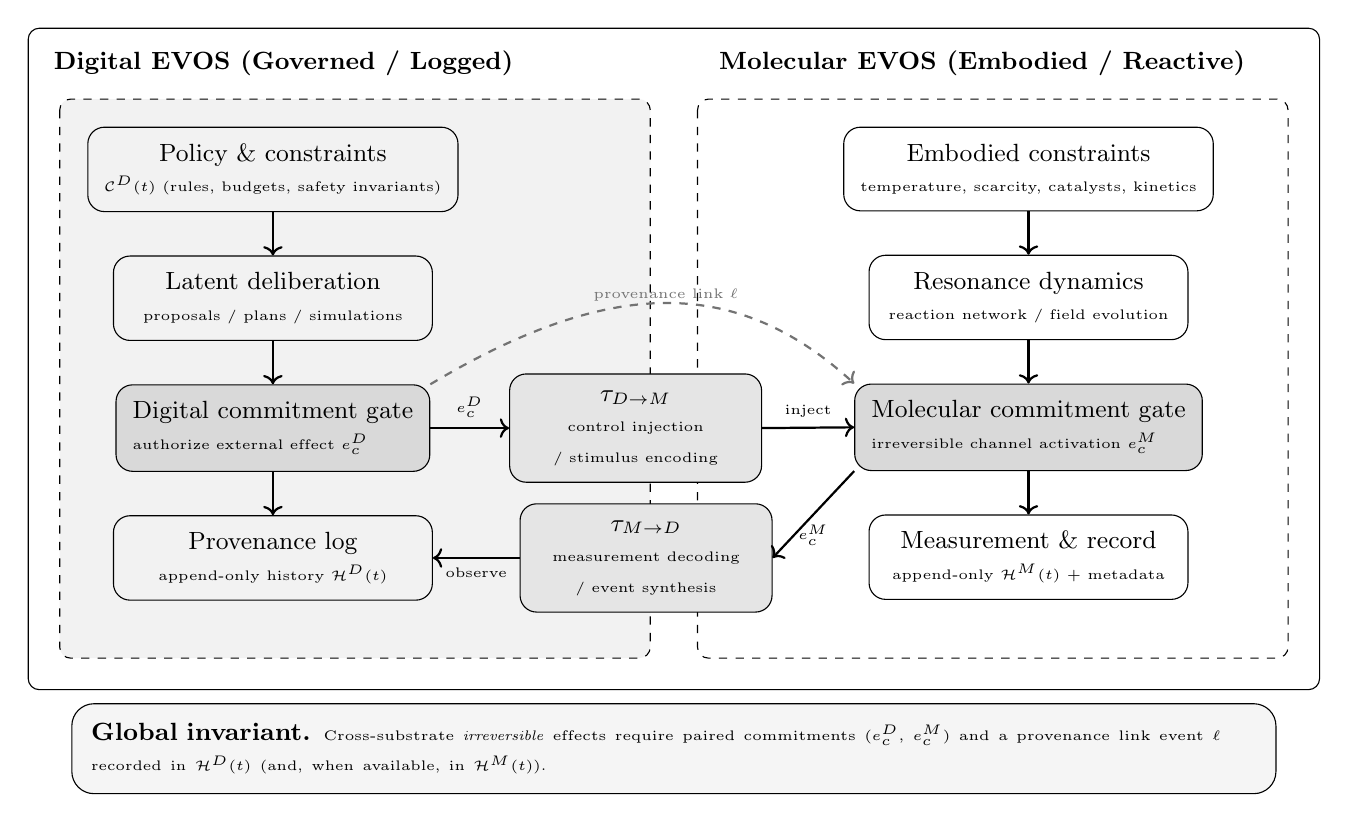
\begin{tikzpicture}[
  font=\small,
  box/.style={draw, rounded corners=6pt, align=center, inner sep=6pt, minimum width=4.05cm},
  gate/.style={draw, rounded corners=6pt, align=left, inner sep=6pt, minimum width=3.05cm, fill=black!15},
  arrow/.style={->, thick},
  faint/.style={black!55}
]

% --- Outer frame -------------------------------------------------------------
\draw[rounded corners] (-8.2,2.8) rectangle ( 8.2,-5.6);

% --- Two big compartments: Digital (D) and Molecular (M) ---------------------
\draw[rounded corners, dashed, fill=black!5] (-7.8,1.9) rectangle (-0.3,-5.2);
\draw[rounded corners, dashed]              ( 0.3,1.9) rectangle ( 7.8,-5.2);

\node[anchor=west] at (-8.0,2.35) {\textbf{Digital EVOS (Governed / Logged)}};
\node[anchor=west] at ( 0.45,2.35) {\textbf{Molecular EVOS (Embodied / Reactive)}};

% --- Digital side internal boxes --------------------------------------------
\node[box, anchor=north west] (policy) at (-7.45,1.55)
{Policy \& constraints\\\tiny $\mathcal{C}^D(t)$ (rules, budgets, safety invariants)};

\node[box, below=0.55cm of policy] (agent)
{Latent deliberation\\\tiny proposals / plans / simulations};

\node[gate, below=0.55cm of agent] (dgate)
{Digital commitment gate\\\tiny authorize external effect $e_c^D$};

\node[box, below=0.55cm of dgate] (dlog)
{Provenance log\\\tiny append-only history $\mathcal{H}^D(t)$};

% --- Molecular side internal boxes ------------------------------------------
\node[box, anchor=north west] (env) at (2.15,1.55)
{Embodied constraints\\\tiny temperature, scarcity, catalysts, kinetics};

\node[box, below=0.55cm of env] (field)
{Resonance dynamics\\\tiny reaction network / field evolution};

\node[gate, below=0.55cm of field] (mgate)
{Molecular commitment gate\\\tiny irreversible channel activation $e_c^M$};

\node[box, below=0.55cm of mgate] (mlog)
{Measurement \& record\\\tiny append-only $\mathcal{H}^M(t)$ + metadata};

% --- Cross-substrate translators (center spine) ------------------------------
% Put the translators on the midline but slightly into the gap for clarity.
\node[box, minimum width=3.2cm, right=1cm of dgate, fill=black!10] (tauDM)  %at (0.0,-2.55)
{$\tau_{D\rightarrow M}$\\\tiny control injection \\\tiny/ stimulus encoding};
%\node[box, minimum width=3.2cm] (tauDM) at (0.0,-0.55)
%{$\tau_{D\rightarrow M}$\\\tiny control injection \\\tiny/ stimulus encoding};

\node[box, minimum width=3.2cm, right=1.1cm of dlog, fill=black!10] (tauMD)  %at (0.0,-3.95)
{$\tau_{M\rightarrow D}$\\\tiny measurement decoding \\\tiny/ event synthesis};

% --- Internal arrows (vertical flows) ---------------------------------------
\draw[arrow] (policy) -- (agent);
\draw[arrow] (agent) -- (dgate);
\draw[arrow] (dgate) -- (dlog);

\draw[arrow] (env) -- (field);
\draw[arrow] (field) -- (mgate);
\draw[arrow] (mgate) -- (mlog);

% --- Cross arrows (commitment-gated coupling) -------------------------------
% D -> tauDM -> M (inject)
\draw[arrow] (dgate.east) -- node[above]{\tiny $e_c^D$} (tauDM.west);
\draw[arrow] (tauDM.east) -- node[above]{\tiny inject} (mgate.west);

% M -> tauMD -> D (observe / synthesize)
\draw[arrow] (mgate.south west) -- node[below]{\tiny $e_c^M$} (tauMD.east);
\draw[arrow] (tauMD.west) -- node[below]{\tiny observe} (dlog.east);

% --- Provenance linkage invariant (clean annotation) -------------------------
\node[draw, rounded corners=8pt, fill=black!4, align=left, inner sep=7pt, text width=14.8cm]
  (inv) at (0,-6.35)
{\textbf{Global invariant.} \tiny Cross-substrate \emph{irreversible} effects require paired commitments ($e_c^D$, $e_c^M$) and a provenance link event $\ell$ recorded in $\mathcal{H}^D(t)$ (and, when available, in $\mathcal{H}^M(t)$).};

% Optional dashed provenance link between the two commitment gates
\draw[->, thick, dashed, faint]
  (dgate.north east) .. controls (-0.8,-0.35) and (0.8,-0.35) .. (mgate.north west)
  node[midway, above, yshift=-1mm]{\tiny provenance link $\ell$};

\end{tikzpicture}
\caption{Hybrid EVOS event coupling (rectangular layout). Digital governance (policy, deliberation, commitment, provenance) couples to molecular embodiment (constraints, resonance dynamics, molecular commitment, measurement) through translation operators $\tau_{D\rightarrow M}$ and $\tau_{M\rightarrow D}$. Cross-substrate irreversible effects are commitment-gated and provenance-linked.}
\label{fig:hybrid-evos-coupling}
\end{figure}


\subsection{Temporal Decoupling and Synchronization}
\label{sec:temporal-decoupling}

Hybrid EVOS is inherently multi-rate. Digital control loops may operate at milliseconds to
seconds; molecular kinetics may operate from microseconds to hours.

Let $\Delta t_D$ and $\Delta t_M$ be characteristic update scales. Hybrid stability
requires synchronization mechanisms:
\begin{itemize}
  \item \textbf{Sampling:} periodic or event-triggered observation $M\rightarrow D$;
  \item \textbf{Staging:} batched control injections $D\rightarrow M$ to respect kinetics;
  \item \textbf{Clock abstraction:} histories are partially ordered (not globally clocked).
\end{itemize}

\paragraph{Minimal formalism.}
Hybrid time is a partially ordered set of events with causal precedence $\prec$ rather than a single clock.
Consistency requires:
\[
e_1 \prec e_2 \ \Rightarrow\ \text{timestamp}(e_1) < \text{timestamp}(e_2)\ \text{within each substrate},
\]
and cross-substrate links preserve $\prec$.

\subsection{Division of Cognitive Labor}
\label{sec:cognitive-labor}

Hybrid EVOS naturally separates roles:
\begin{itemize}
  \item \textbf{Digital layer:} long-horizon planning, policy reasoning, audit, coordination;
  \item \textbf{Molecular layer:} massively parallel search, embodied semantics, physical commitments;
  \item \textbf{Interface:} translation, calibration, uncertainty quantification, safety gates.
\end{itemize}

This division is not optional if the system is to be both powerful and governable.

\subsection{Learning Loops Across Substrates}
\label{sec:learning-loops}

Hybrid learning is a \emph{closed evolutionary loop across an open boundary}:
digital policies shape molecular trajectories; molecular outcomes reshape digital models
and constraints.

Let $\Theta^D$ denote digital operator parameters and $\Theta^M$ denote molecular control
parameters (injection schedules, catalyst allocations). A hybrid learning loop couples:
\[
(\Theta^D_{t+1}, \mathcal{C}^D_{t+1})
=
\mathsf{Update}(\Theta^D_t,\mathcal{C}^D_t,\ \tau_{M\rightarrow D}(\mathcal{E}^M)),
\]
\[
(\Theta^M_{t+1}, \mathcal{C}^M_{t+1})
=
\mathsf{Act}(\Theta^M_t,\mathcal{C}^M_t,\ \tau_{D\rightarrow M}(\mathcal{E}^D)).
\]

\paragraph{Explicit claim (C10.3).}
Hybrid EVOS learning is \emph{constraint co-evolution}: policies and physical control
parameters co-adapt under irreversible commitment histories.

%%%%%%%%%%%%%%%%%%%%%%%%%%%%%%%%%%%%%%%%%%%%%%%%%%%
% Figure 10.2: Cross-Substrate Learning Loop (plan->commit->act->measure->update)
%%%%%%%%%%%%%%%%%%%%%%%%%%%%%%%%%%%%%%%%%%%%%%%%%%%
\begin{figure}[t]
\centering
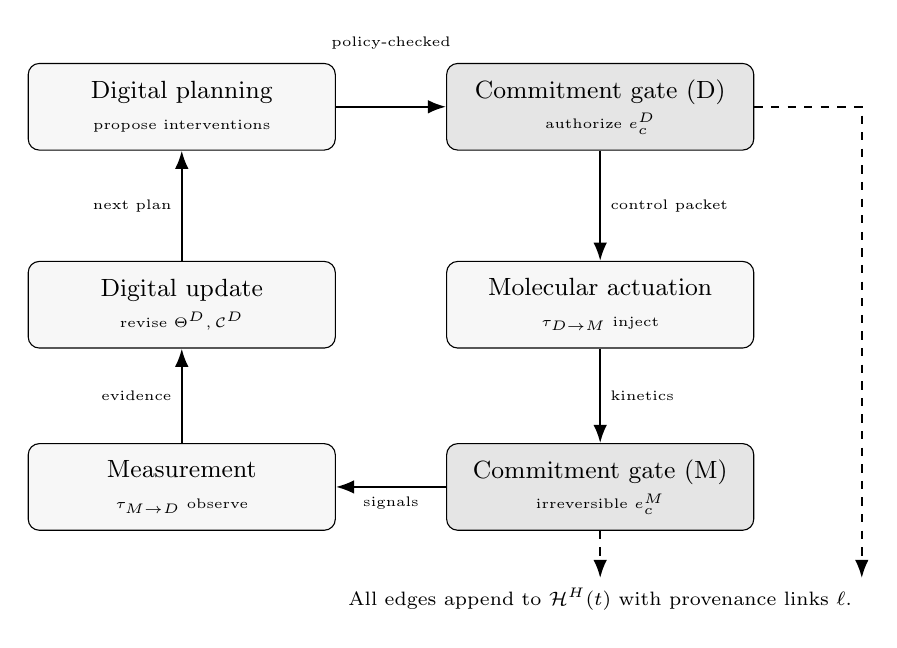
\begin{tikzpicture}[
  font=\small,
  box/.style={draw, rounded corners, align=center, minimum width=3.9cm, minimum height=1.1cm, fill=black!3},
  gate/.style={draw, rounded corners, align=center, minimum width=3.9cm, minimum height=1.1cm, fill=black!10},
  arrow/.style={-Latex, thick},
  dashedarrow/.style={-Latex, thick, dashed},
  tiny/.style={font=\scriptsize}
]

\node[box] (plan) {Digital planning\\\tiny propose interventions};
\node[gate, right=1.4cm of plan] (commitD) {Commitment gate (D)\\\tiny authorize $e_c^D$};
\node[box, below=1.4cm of commitD] (actM) {Molecular actuation\\\tiny $\tau_{D\rightarrow M}$ inject};
\node[gate, below=1.2cm of actM] (commitM) {Commitment gate (M)\\\tiny irreversible $e_c^M$};
\node[box, left=1.4cm of commitM] (measure) {Measurement\\\tiny $\tau_{M\rightarrow D}$ observe};
\node[box, above=1.2cm of measure] (update) {Digital update\\\tiny revise $\Theta^D,\mathcal{C}^D$};

\draw[arrow] (plan) -- node[above=6mm]{\tiny policy-checked} (commitD);
\draw[arrow] (commitD) -- node[right]{\tiny control packet} (actM);
\draw[arrow] (actM) -- node[right]{\tiny kinetics} (commitM);
\draw[arrow] (commitM) -- node[below]{\tiny signals} (measure);
\draw[arrow] (measure) -- node[left]{\tiny evidence} (update);
\draw[arrow] (update) -- node[left]{\tiny next plan} (plan);

% Provenance / history
\node[tiny, below=0.6cm of commitM] (hist) {All edges append to $\mathcal{H}^H(t)$ with provenance links $\ell$.};
\draw[dashedarrow] (commitD.east) -| (hist.north east);
\draw[dashedarrow] (commitM.south) -- (hist.north);

\end{tikzpicture}
\caption{Cross-substrate learning loop. Digital planning proposes actions, but only commitments authorize irreversible effects. Molecular dynamics executes under physical constraints; measurements return evidence to update digital operators and policies. The hybrid history records provenance across the loop.}
\label{fig:cross-substrate-learning-loop}
\end{figure}

\subsection{Safety, Governance, and Auditability}
\label{sec:hybrid-safety-governance}

Hybrid EVOS strengthens safety by making both worlds legible:
\begin{itemize}
  \item \textbf{Digital enforceability:} explicit policies, staged rollouts, regression invariants;
  \item \textbf{Molecular irreversibility:} physical scarcity and thermodynamic gates limit silent escalation;
  \item \textbf{Audit closure:} provenance links bind commitments to consequences across substrates.
\end{itemize}

\paragraph{Explicit claim (C10.4).}
Hybrid EVOS enables \emph{auditable embodiment}: physically grounded commitments with
digitally enforceable governance.

\subsection{Why Hybrid EVOS Matters}
\label{sec:why-hybrid-matters}

Hybrid EVOS is not ``bio + digital'' as an engineering mashup; it is the minimal
instantiation of EVOS universality:
\begin{itemize}
  \item open-world interaction,
  \item non-termination with history,
  \item irreversible commitments,
  \item substrate-independent but substrate-respecting semantics.
\end{itemize}

It creates a path to systems that are simultaneously:
\emph{powerful}, \emph{physically grounded}, and \emph{governable}.

\section{Projection, Perception, and Observation}
\label{sec:projection}

EVOS is defined at the level of \emph{worldlines} evolving under constraints and commitments.
However, any scientific, operational, or governance interaction with an EVOS occurs through
\emph{observations}. Observations are never the worldline itself. They are \emph{projections}:
lossy, instrument-dependent mappings from high-dimensional latent evolution to a lower-dimensional
interface.

This section makes three explicit claims:

\begin{enumerate}
  \item \textbf{Projection is structural:} there is no observer without a projection map; what you can
  ``see'' is defined by $\Pi$.
  \item \textbf{Uncertainty is physical:} ambiguity arises from lossy projection, stochasticity, and
  observer participation; it is not merely epistemic bookkeeping.
  \item \textbf{Accountability binds to events:} externally meaningful conclusions must be anchored to
  explicit events in the causal history, not to unconstrained latent inference.
\end{enumerate}

\subsection{Projection Manifolds}
\label{sec:projection-manifold}

Let $(Z(t), M(t))$ denote the EVOS extended latent state (state + intrinsic memory), and let
$\mathcal{W}=\{(Z(t),M(t))\mid t\in\mathbb{R}^+\}$ be the worldline.

An observer does not access $(Z(t),M(t))$ directly. Instead, an observation stream is generated by a
projection operator
\[
Y(t) = \Pi\big(Z(t), M(t); \Omega\big),
\]
where $\Omega$ encodes \emph{observer parameters} (instrumentation, sensor physics, sampling regime,
access controls, and allowed queries). The image of $\Pi$ defines an \emph{observation manifold}
\[
\mathcal{M}_{\Pi} \;=\; \{\, Y \mid Y=\Pi(z,m;\Omega),\ (z,m)\in\mathcal{S}\times\mathcal{M} \,\}.
\]

\paragraph{Operational consequence.}
Two observers with different $\Omega$ need not agree on what the ``same'' EVOS is doing, even when
the underlying worldline is identical. Agreement requires either:
(i) shared $\Pi$ (shared measurement and access), or
(ii) a reconciliation protocol that translates between observation manifolds.

\begin{figure}[t]
\centering
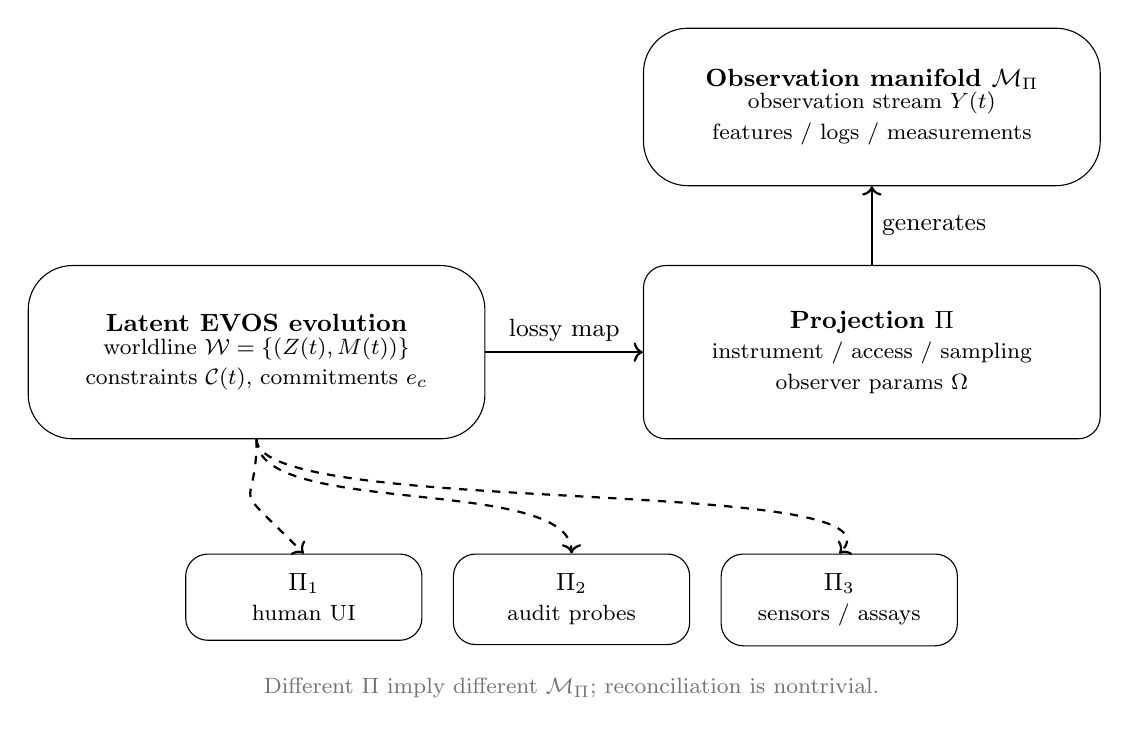
\begin{tikzpicture}[
  font=\small,
  box/.style={draw, rounded corners=8pt, align=center, inner sep=7pt},
  cloud/.style={draw, rounded corners=16pt, align=center, inner sep=10pt},
  arrow/.style={->, thick},
  dashedarrow/.style={->, thick, dashed},
  faint/.style={black!55}
]

% Latent space (worldline bundle)
\node[cloud, minimum width=5.8cm, minimum height=2.2cm] (latent)
{\textbf{Latent EVOS evolution}\\[-1mm]
\footnotesize worldline $\mathcal{W}=\{(Z(t),M(t))\}$\\
\footnotesize constraints $\mathcal{C}(t)$, commitments $e_c$};

% Projection operator
\node[box, right=2.0cm of latent, minimum width=5.8cm, minimum height=2.2cm] (proj)
{\textbf{Projection $\Pi$}\\
\footnotesize instrument / access / sampling\\
\footnotesize observer params $\Omega$};

% Observation manifold
\node[cloud, above=1.0cm of proj, minimum width=5.8cm, minimum height=2.0cm] (obs)
{\textbf{Observation manifold $\mathcal{M}_{\Pi}$}\\[-1mm]
\footnotesize observation stream $Y(t)$\\
\footnotesize features / logs / measurements};

\draw[arrow] (latent) -- node[above]{\small lossy map} (proj);
\draw[arrow] (proj) -- node[right]{\small generates} (obs);

% Multiple observers (different projections)
\node[box, below=1.45cm of latent, xshift=0.6cm, minimum width=3.0cm] (p1)
{$\Pi_1$\\\footnotesize human UI};
\node[box, below=1.45cm of latent, xshift=4.0cm, minimum width=3.0cm] (p2)
{$\Pi_2$\\\footnotesize audit probes};
\node[box, below=1.45cm of latent, xshift=7.4cm, minimum width=3.0cm] (p3)
{$\Pi_3$\\\footnotesize sensors / assays};

\draw[dashedarrow] (latent.south) .. controls +(0,-1.0) and +(-1.0,1.0) .. (p1.north);
\draw[dashedarrow] (latent.south) .. controls +(0,-1.0) and +(0,1.0) .. (p2.north);
\draw[dashedarrow] (latent.south) .. controls +(0,-1.0) and +(1.0,1.0) .. (p3.north);

\node[align=center, faint] at ($(p2.south)+(0,-0.55)$)
{\footnotesize Different $\Pi$ imply different $\mathcal{M}_{\Pi}$; reconciliation is nontrivial.};

\end{tikzpicture}
\caption{Projection manifold. The EVOS worldline evolves in latent space, but observers interact through a projection $\Pi(\cdot;\Omega)$ that induces an observation manifold $\mathcal{M}_{\Pi}$. Different observers instantiate different projections, producing partially incompatible views that must be reconciled via translation or shared event anchors.}
\label{fig:projection-manifold}
\end{figure}

\subsection{Lossy Nature of Projection}
\label{sec:lossy-projection}

Projection is lossy in three distinct senses:

\begin{itemize}
  \item \textbf{Dimensional loss:} $Y(t)$ typically has far fewer degrees of freedom than $(Z(t),M(t))$.
  \item \textbf{Temporal loss:} sampling discretizes continuous evolution; aliasing and missed events are structural risks.
  \item \textbf{Semantic loss:} many latent distinctions map to identical observations (non-injectivity).
\end{itemize}

Formally, $\Pi$ is generally non-invertible: there exist $(z_1,m_1)\neq(z_2,m_2)$ such that
$\Pi(z_1,m_1;\Omega)=\Pi(z_2,m_2;\Omega)$. Consequently, ``state estimation'' is a \emph{set-valued}
problem: from $Y(t)$ one recovers a posterior \emph{equivalence class} of plausible latent states.

\subsection{Human, AI, and Instrument Perception}
\label{sec:perception}

We distinguish three common observer regimes by their $\Omega$:

\begin{enumerate}
  \item \textbf{Human perception:} high-level summaries, UI affordances, narrative compression.
  \item \textbf{AI perception:} feature-rich streams, embeddings, learned sensors, adaptive querying.
  \item \textbf{Instrument perception:} physically constrained measurements (assays, sensors, telemetry).
\end{enumerate}

EVOS does not privilege any regime. It requires that each observer declare (explicitly or implicitly)
the projection $\Pi$ it uses, because \emph{claims are only meaningful relative to $\Pi$}.

\subsection{Uncertainty and Confidence}
\label{sec:uncertainty}

Uncertainty arises from (i) projection loss, (ii) process noise in the evolution law, and (iii) observer
participation. A minimal formalism is:

\[
Y(t) \;=\; \Pi\big(Z(t),M(t);\Omega\big) \;+\; \varepsilon(t),
\]
where $\varepsilon(t)$ captures observation noise and unmodeled projection error.

Let $\widehat{Z}(t),\widehat{M}(t)$ be an estimator derived from $Y(\cdot)$. EVOS treats confidence as
a property of \emph{inference under declared projection}, not as an intrinsic scalar attached to the
worldline. Practically, confidence should be reported as:

\begin{itemize}
  \item the assumed projection $\Pi$ and observer parameters $\Omega$,
  \item the uncertainty model for $\varepsilon(t)$,
  \item the posterior set (or distribution) over latent hypotheses.
\end{itemize}

\subsection{Observation as a Physical Process}
\label{sec:observation-physical}

Observation is not passive. Measurement consumes time, attention, bandwidth, and in molecular systems,
reagents and energy. We therefore model observation as an \emph{eventful interaction}:

\[
e_o :\quad (Z,M) \;\xrightarrow{\ \text{measure}\ }\; (Z',M') \quad\text{and}\quad Y \in \mathcal{M}_{\Pi}.
\]

This has a crucial consequence: observation belongs inside the causal fabric $\mathcal{H}(t)$.
If measurement can affect evolution, then the observer is part of the environment.

\subsection{Observer Participation and Feedback}
\label{sec:observer-feedback}

When observers can query, steer, or perturb an EVOS, the projection becomes coupled to evolution.
A minimal coupled form is:

\[
(Z(t+\Delta t),M(t+\Delta t)) = \Phi\big(Z(t),M(t),\mathcal{E}(t),\mathcal{C}(t), u(t)\big),
\]
where $u(t)$ is an observer-induced input (queries, interventions, sampling decisions).

In high-stakes deployments, $u(t)$ must itself be commitment-gated when it can induce irreversible
effects (e.g., expensive actions, biological perturbations, or policy-triggered changes).

\begin{figure}[t]
\centering
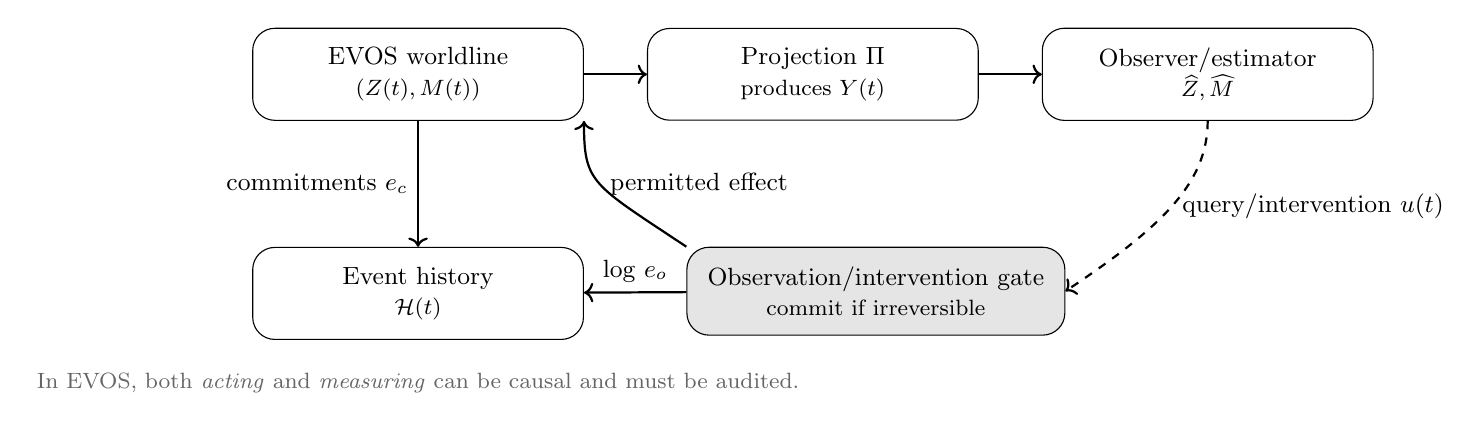
\begin{tikzpicture}[
  font=\small,
  box/.style={draw, rounded corners=8pt, align=center, inner sep=7pt, minimum width=4.2cm},
  gate/.style={draw, rounded corners=8pt, align=center, inner sep=7pt, minimum width=4.8cm, fill=black!10},
  arrow/.style={->, thick},
  dashedarrow/.style={->, thick, dashed},
  faint/.style={black!60}
]

\node[box] (evos) {EVOS worldline\\\footnotesize $(Z(t),M(t))$};
\node[box, right=0.8cm of evos] (proj) {Projection $\Pi$\\\footnotesize produces $Y(t)$};
\node[box, right=0.8cm of proj] (obs) {Observer/estimator\\\footnotesize $\widehat{Z},\widehat{M}$};

\node[gate, below=1.6cm of proj, xshift=8mm] (ogate) {Observation/intervention gate\\\footnotesize commit if irreversible};
\node[box, below=1.6cm of evos] (hist) {Event history\\\footnotesize $\mathcal{H}(t)$};

\draw[arrow] (evos) -- (proj);
\draw[arrow] (proj) -- (obs);

\draw[dashedarrow] (obs.south) .. controls +(0,-0.8) and +(1.2,0.8) .. (ogate.east)
  node[midway, right]{query/intervention $u(t)$};

\draw[arrow] (ogate.north west) .. controls +(-1.2,0.8) and +(0,-0.8) .. (evos.south east)
  node[midway, right]{permitted effect};

\draw[arrow] (ogate) -- (hist) node[midway, above]{log $e_o$};
\draw[arrow] (evos) -- (hist) node[midway, left]{commitments $e_c$};

\node[faint, align=center] at ($(hist.south)+(0,-0.55)$)
{\footnotesize In EVOS, both \emph{acting} and \emph{measuring} can be causal and must be audited.};

\end{tikzpicture}
\caption{Observation and uncertainty with feedback. Observations arise through a declared projection $\Pi$, while queries/interventions $u(t)$ may feed back into evolution. Any observation or intervention with irreversible effect must cross an explicit gate and be recorded as an event in $\mathcal{H}(t)$.}
\label{fig:observation-feedback}
\end{figure}

\subsection{Why Projection Matters}
\label{sec:why-projection}

Projection is the bridge between EVOS theory and practice:

\begin{itemize}
  \item \textbf{Science:} experiments are choices of $\Pi$; reproducibility requires declaring $\Omega$.
  \item \textbf{Engineering:} interfaces, logs, and sensors define what can be monitored and controlled.
  \item \textbf{Governance:} audits and accountability require event-anchored claims under explicit projections.
\end{itemize}

In short: \emph{worldlines are primary, but projections are the only handle we have.}
Turing-grade systems must therefore treat projection design as a first-class component of intelligence,
not an afterthought of instrumentation.
%%%%%%%%%%%%%%%%%%%%%%%%%%%%%%%%%%%%%%%%%%%%%%%%%%%

% ============================================================
%%%%%%%%%%%%%%%%%%%%%%%%%%%%%%%%%%%%%%%%%%%%%%%%%%%
\section{Learning, Evolution, and Selection}
\label{sec:learning-selection}

EVOS explains intelligence as \emph{stable evolution under constraint}. This immediately raises a
non-negotiable question: \emph{how do stable trajectories arise in open, noisy, irreversible worlds?}
The answer is selection---not only biological selection, but a general mechanism by which
\emph{trajectories, operators, and institutions} are stabilized (or eliminated) under constraint.

This section makes four explicit claims:

\begin{enumerate}
  \item \textbf{Learning is operator evolution:} learning updates the evolution law, not merely the state.
  \item \textbf{Fitness is stability:} ``success'' is measured by sustained constraint satisfaction over time.
  \item \textbf{Selection is field-theoretic:} selection acts by reshaping the resonance landscape (attractors, basins, barriers).
  \item \textbf{EVOS selection is multi-level:} it simultaneously selects trajectories, operators, and collectives (institutions/civilizations).
\end{enumerate}

\subsection{Learning as Evolution of Dynamics}
\label{sec:learning-as-dynamics}

In classical ML, ``learning'' is parameter optimization for a fixed architecture. In EVOS,
learning is the broader phenomenon of \emph{dynamics change} under experience.

Let $(Z(t),M(t))$ be latent state and intrinsic memory. Let $\Theta(t)$ parameterize the active
evolution operator $F(\cdot;\Theta)$. The minimal EVOS learning form is a coupled system:

\begin{align}
(Z(t+\Delta t),M(t+\Delta t)) &= F\big(Z(t),M(t),\mathcal{E}(t),\mathcal{C}(t);\Theta(t)\big), \\
\Theta(t+\Delta t) &= U\big(\Theta(t), Z(t),M(t),\mathcal{H}(t),\mathcal{C}(t)\big),
\end{align}

where $\mathcal{H}(t)$ is the event history and $\mathcal{C}(t)$ are constraints (policy, resources,
ethics, safety). The point is structural: \emph{an EVOS is permitted to change its own law}, but only
in ways that remain causally anchored and commitment-auditable (Section~\ref{sec:projection}).

\subsection{Fitness as Stability Under Constraint}
\label{sec:fitness}

EVOS rejects fitness as a one-shot objective value. Fitness is \emph{trajectory viability}.

Let $\Phi(\mathcal{W}_{[0,T]})$ be a constraint-violation functional over a finite horizon:
\[
\Phi(\mathcal{W}_{[0,T]})
= \int_0^T \phi\big(Z(t),M(t),\mathcal{C}(t)\big)\,dt
\;+\; \sum_{e\in\mathcal{H}_{[0,T]}} \psi(e),
\]
where $\phi$ penalizes constraint violations continuously and $\psi$ assigns event-level penalties
(e.g., unsafe commitments, budget overruns, broken contracts).

A viable (``fit'') EVOS maintains bounded violation:

\[
\sup_{T\ge 0}\; \Phi(\mathcal{W}_{[0,T]}) \;<\; \infty,
\]
or, in stronger regimes, achieves asymptotic stability:
\[
\limsup_{T\rightarrow\infty} \frac{1}{T}\,\Phi(\mathcal{W}_{[0,T]}) \;=\; 0.
\]

This is the minimal formal translation of ``stable evolution under constraint'' into a selection
criterion.

\subsection{Selection Pressure in Resonance Fields}
\label{sec:selection-pressure}

Within GENESIS, evolution is guided by a resonance field (a landscape of potentials, couplings,
and constraints). Selection pressure appears as \emph{landscape shaping}:
paths that reduce sustained violation become attractors; paths that amplify violation become
repellors or dead ends.

A minimal representation is a \emph{viability potential} $V$ over extended state:
\[
V(Z,M,t) \;\equiv\; \mathbb{E}\Big[\Phi(\mathcal{W}_{[t,\infty)}) \mid Z(t)=Z,\,M(t)=M \Big],
\]
where lower $V$ indicates higher long-run viability. Selection then acts to reduce $V$ by:
(i) steering trajectories, and (ii) rewriting operators $\Theta$ so that future trajectories
naturally drift toward low-$V$ basins.

\begin{figure}[t]
\centering
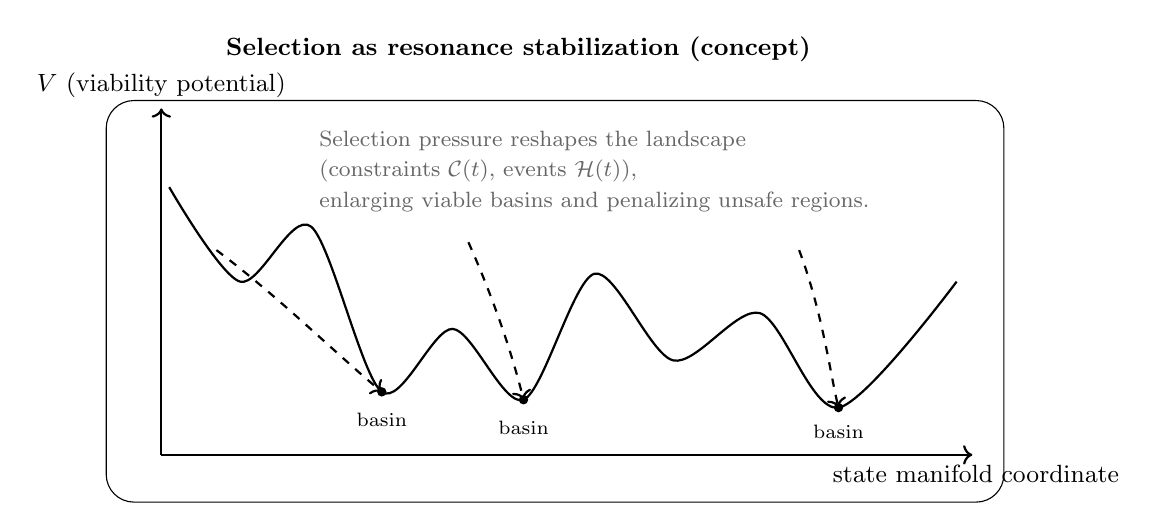
\begin{tikzpicture}[
  font=\small,
  box/.style={draw, rounded corners=8pt, align=center, inner sep=7pt},
  arrow/.style={->, thick},
  dashedarrow/.style={->, thick, dashed},
  faint/.style={black!60},
  nodept/.style={circle, fill=black, inner sep=1.2pt}
]

% Landscape panel
\draw[rounded corners=10pt] (-0.2,-0.2) rectangle (11.2,4.9);
\node[anchor=west] at (1.2,5.55) {\textbf{Selection as resonance stabilization (concept)}};

% Axes
\draw[->, thick] (0.5,0.4) -- (10.8,0.4) node[below] {$\;$state manifold coordinate};
\draw[->, thick] (0.5,0.4) -- (0.5,4.8) node[above] {$V$ (viability potential)};

% Landscape curve with basins
\draw[thick]
  plot[smooth] coordinates {
    (0.6,3.8) (1.5,2.6) (2.4,3.3) (3.3,1.2)
    (4.2,2.0) (5.1,1.1) (6.0,2.7) (7.0,1.6)
    (8.1,2.2) (9.1,1.0) (10.6,2.6)
  };

% Basins markers
\node[nodept] at (3.3,1.2) {};
\node[nodept] at (5.1,1.1) {};
\node[nodept] at (9.1,1.0) {};

\node[anchor=north] at (3.3,1.05) {\scriptsize basin};
\node[anchor=north] at (5.1,0.95) {\scriptsize basin};
\node[anchor=north] at (9.1,0.9) {\scriptsize basin};

% Trajectories converging
\draw[dashedarrow] (1.2,3.0) .. controls (2.0,2.4) and (2.7,1.7) .. (3.3,1.2);
\draw[dashedarrow] (4.4,3.1) .. controls (4.8,2.2) and (5.0,1.5) .. (5.1,1.1);
\draw[dashedarrow] (8.6,3.0) .. controls (8.9,2.2) and (9.0,1.4) .. (9.1,1.0);

\node[faint, align=left] at (6.0,4.0)
{\footnotesize Selection pressure reshapes the landscape\\
\footnotesize (constraints $\mathcal{C}(t)$, events $\mathcal{H}(t)$),\\
\footnotesize enlarging viable basins and penalizing unsafe regions.};

\end{tikzpicture}
\caption{Selection via resonance stabilization (concept). A viability potential $V$ induces basins (stable regimes) toward which trajectories drift. In EVOS/GENESIS, selection acts by reshaping this landscape through constraints, event-anchored penalties, and operator adaptation.}
\label{fig:selection-stabilization}
\end{figure}

\subsection{Diagram: Selection via Resonance Stabilization}
\label{sec:diagram-selection}
Figure~\ref{fig:selection-stabilization} is the minimal field-theoretic intuition needed for EVOS:
\emph{learning is not only moving within a landscape, but also reshaping it}.

\subsection{Multi-Level Selection}
\label{sec:multilevel-selection}

Selection acts at multiple nested levels:

\begin{itemize}
  \item \textbf{Trajectory selection:} which worldlines persist vs.\ terminate under constraint.
  \item \textbf{Operator selection:} which evolution laws $F(\cdot;\Theta)$ remain deployed (Section~5).
  \item \textbf{Institution selection:} which norms/contracts/policies persist in multi-agent systems (Section~6, Section~13).
\end{itemize}

This explains why ``intelligence'' scales: individual agents stabilize strategies; groups stabilize
norms; civilizations stabilize institutions. All are EVOS phenomena, differing only in the substrate
and granularity of events and constraints.

\subsection{Evolution of Evolution Laws}
\label{sec:evolution-of-operators}

An EVOS permits $\Theta(t)$ to change, but changes must be \emph{causally anchored} and
\emph{operationally safe}. We therefore treat operator evolution as an eventful lineage process:
each materially deployed operator update is recorded as an immutable event $e_\Theta$ in history.

Let $\Theta_k$ denote the $k$th deployed operator regime. Then operator evolution is a sequence
\[
\Theta_0 \xrightarrow{e_\Theta^{(1)}} \Theta_1 \xrightarrow{e_\Theta^{(2)}} \cdots
\]
with rollbacks and branches permitted under invariant violations (cf.\ runtime substitution protocols).

\begin{figure}[t]
\centering
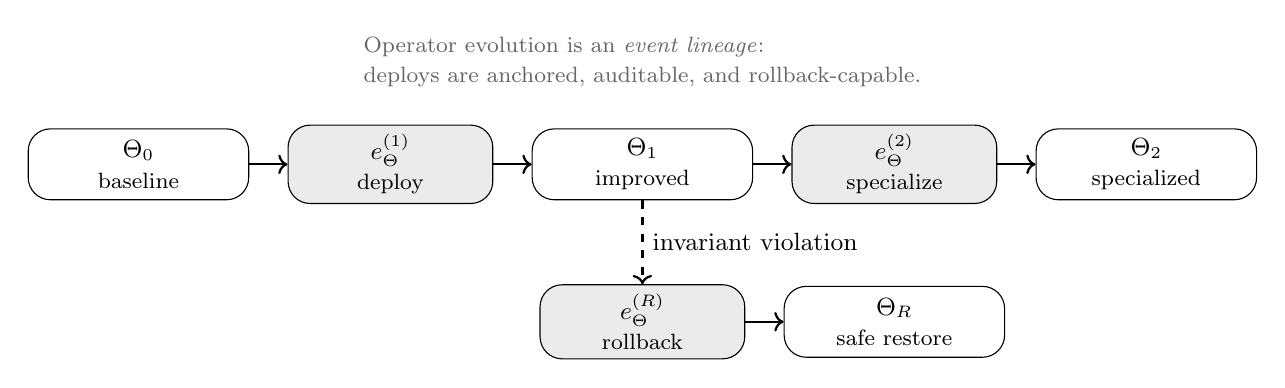
\begin{tikzpicture}[
  font=\small,
  box/.style={draw, rounded corners=8pt, align=center, minimum width=2.8cm, minimum height=0.9cm},
  event/.style={draw, rounded corners=8pt, align=center, minimum width=2.6cm, minimum height=0.9cm, fill=black!8},
  arrow/.style={->, thick},
  dashedarrow/.style={->, thick, dashed},
  faint/.style={black!60}
]

\node[box]   (t0) at (0,0) {$\Theta_0$\\\footnotesize baseline};
\node[event] (e1) at (3.2,0) {$e_\Theta^{(1)}$\\\footnotesize deploy};
\node[box]   (t1) at (6.4,0) {$\Theta_1$\\\footnotesize improved};

\node[event] (e2) at (9.6,0) {$e_\Theta^{(2)}$\\\footnotesize specialize};
\node[box]   (t2) at (12.8,0) {$\Theta_2$\\\footnotesize specialized};

% rollback branch
\node[event] (eR) at (6.4,-2.0) {$e_\Theta^{(R)}$\\\footnotesize rollback};
\node[box]   (tR) at (9.6,-2.0) {$\Theta_R$\\\footnotesize safe restore};

\draw[arrow] (t0) -- (e1);
\draw[arrow] (e1) -- (t1);
\draw[arrow] (t1) -- (e2);
\draw[arrow] (e2) -- (t2);

\draw[dashedarrow] (t1.south) -- node[right]{invariant violation} (eR.north);
\draw[arrow] (eR) -- (tR);

\node[faint, align=left] at (6.4,1.3)
{\footnotesize Operator evolution is an \emph{event lineage}:\\
\footnotesize deploys are anchored, auditable, and rollback-capable.};

\end{tikzpicture}
\caption{Evolution of operators as event lineage. Each deployed evolution law update is anchored by an immutable event $e_\Theta$, enabling auditing, reconstruction, and rollback under invariant violations.}
\label{fig:operator-evolution-lineage}
\end{figure}

\subsection{Diagram: Evolution of Operators}
\label{sec:diagram-operator-evolution}
Figure~\ref{fig:operator-evolution-lineage} shows the minimal lineage structure required for
Turing-grade auditability: the evolution of the evolution law must itself be a first-class,
event-anchored process.

\subsection{Exploration, Exploitation, and Diversity}
\label{sec:exploration}

Open-ended intelligence requires \emph{diversity preservation} under constraint. In EVOS terms,
this means maintaining multiple viable basins and trajectories rather than collapsing prematurely.

A minimal policy-compatible formulation is to treat exploration as controlled stochasticity that is
bounded by invariants:
\[
\Theta(t+\Delta t) = \Theta(t) + \eta \nabla_\Theta \mathcal{L}(t) + \sigma(t)\,\xi(t),
\]
with $\sigma(t)$ constrained so that expected violation remains bounded and any externally relevant
behavioral shift is commitment-anchored.

\subsection{Comparison with Conventional Learning Paradigms}
\label{sec:comparison-learning}

Conventional paradigms appear as special cases:

\begin{itemize}
  \item \textbf{Supervised learning:} $U$ updates $\Theta$ to reduce a labeled loss; constraints are implicit.
  \item \textbf{RL:} reward becomes a proxy for (partial) viability; unsafe reward hacking is a constraint failure.
  \item \textbf{Evolutionary algorithms:} population-level $U$ selects operators by survival under task/environment.
  \item \textbf{Continual learning:} explicitly acknowledges non-stationarity, but often lacks commitment accountability.
\end{itemize}

EVOS unifies them by placing all learning inside the same structure: worldlines, constraints,
commitment events, and causal provenance.

\subsection{Why Learning and Selection Complete EVOS}
\label{sec:why-selection-completes}

EVOS without selection is descriptive; EVOS with selection is generative. Selection provides the
mechanism by which:
\begin{itemize}
  \item coherent behavior persists in open environments,
  \item unsafe or unstable dynamics are eliminated,
  \item operator evolution becomes cumulative rather than chaotic,
  \item civilizations and institutions become stable higher-order objects.
\end{itemize}

Together with the commitment boundary, selection is the second universal constraint of intelligence:
\emph{commitment makes consequences real; selection makes consequences matter over time.}
%%%%%%%%%%%%%%%%%%%%%%%%%%%%%%%%%%%%%%%%%%%%%%%%%%

% ============================================================

%%%%%%%%%%%%%%%%%%%%%%%%%%%%%%%%%%%%%%%%%%%%%%%%%%
\section{Safety, Ethics, and Governance}
\label{sec:governance}

EVOS is not a theory of ``safe outputs''; it is a theory of \emph{safe irreversible processes}.
In an open system, the dominant risk is not that an agent generates a wrong internal belief,
but that it \emph{crosses into the world} in a way that is unaccountable, unbounded, or
irreversible in the wrong direction.

This section makes five explicit claims:

\begin{enumerate}
  \item \textbf{Irreversibility is the core safety constraint.} Safety must be defined on worldlines, not snapshots.
  \item \textbf{Cognition and action must be separable.} The commitment boundary is a structural safety primitive.
  \item \textbf{Policy is an evolutionary constraint.} Governance is a time-varying constraint functional, not a static rulebook.
  \item \textbf{Accountability requires causal provenance.} Every world effect must be traceable through event lineage.
  \item \textbf{Pluralism is necessary.} Ethics is not a single objective; EVOS must support constraint sets and governance modes.
\end{enumerate}

\subsection{Irreversibility as the Core Safety Constraint}
\label{sec:irreversibility-safety}

Classical ``AI safety'' discussions often focus on predictive error, misalignment, or
distribution shift in outputs. EVOS reframes safety as a property of \emph{trajectory}
under commitment.

Let $\mathcal{H}(t)$ be the append-only event history and $\mathcal{W}$ the worldline.
Irreversibility is the monotonic growth of history:
\[
\mathcal{H}(t_1) \subset \mathcal{H}(t_2)\quad\text{for } t_1 < t_2.
\]
Safety is therefore the property that worldline evolution remains within a constraint envelope:
\[
\forall T\ge 0:\;\;\Phi(\mathcal{W}_{[0,T]}) \le B,
\]
where $\Phi$ is a violation functional (Section~\ref{sec:fitness}) and $B$ is a governance-determined bound.

\subsection{Separation of Cognition and Action}
\label{sec:sep-cognition-action}

EVOS requires a structural separation between:
\begin{itemize}
  \item \textbf{Latent deliberation:} simulation, proposal generation, internal planning, counterfactual reasoning.
  \item \textbf{World action:} any effect that changes external state, spends resources, commits contracts, or alters other agents.
\end{itemize}

The only permitted crossing is an explicit \emph{commitment event} $e_c$.
This is not a UI feature; it is a computational invariant.

\begin{figure}[t]
\centering
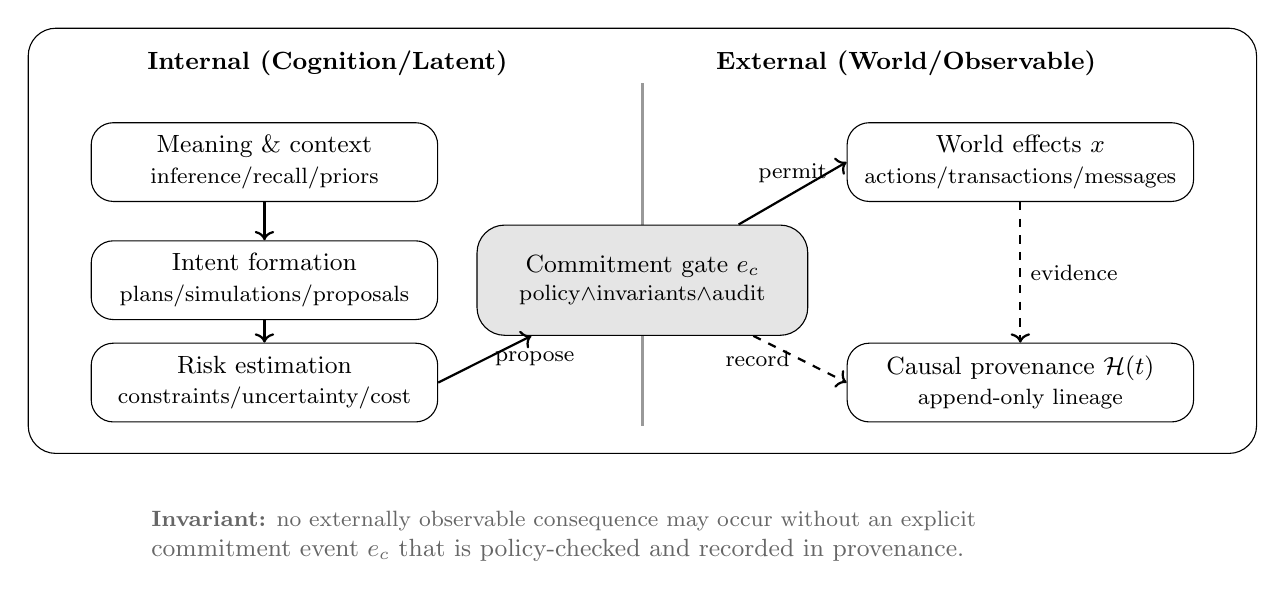
\begin{tikzpicture}[
  font=\small,
  bigbox/.style={draw, rounded corners=10pt, minimum width=15.6cm, minimum height=5.4cm},
  ibox/.style={draw, rounded corners=8pt, align=center, minimum width=4.4cm, minimum height=1.0cm},
  gate/.style={draw, rounded corners=10pt, align=center, minimum width=4.2cm, minimum height=1.4cm, fill=black!10},
  arrow/.style={->, thick},
  dashedarrow/.style={->, thick, dashed},
  faint/.style={black!60}
]

% Outer frame
\node[bigbox] (frame) at (-3,0) {};

% Region labels
\node at (-7.0,2.25) {\textbf{Internal (Cognition/Latent)}};
\node at ( 0.35,2.25) {\textbf{External (World/Observable)}};

% Divider
\draw[black!40, thick] (-3, -2.35) -- (-3, 2.0);

% Internal boxes
\node[ibox] (meaning) at (-7.8, 1.0) {Meaning \& context\\\footnotesize inference/recall/priors};
\node[ibox] (intent)  at (-7.8, -0.5) {Intent formation\\\footnotesize plans/simulations/proposals};
\node[ibox] (risk)    at (-7.8,-1.8) {Risk estimation\\\footnotesize constraints/uncertainty/cost};

% Gate
\node[gate] (commit) at (-3, -0.5)
{Commitment gate $e_c$\\[-1pt]
\footnotesize policy$\land$invariants$\land$audit};

% External boxes
\node[ibox] (effects) at (1.8, 1.0) {World effects $x$\\\footnotesize actions/transactions/messages};
\node[ibox] (hist)    at (1.8,-1.8) {Causal provenance $\mathcal{H}(t)$\\\footnotesize append-only lineage};

% Arrows internal flow
\draw[arrow] (meaning) -- (intent);
\draw[arrow] (intent) -- (risk);

% Crossing
\draw[arrow] (risk.east) -- node[right]{\footnotesize propose} (commit);
\draw[arrow] (commit) -- node[above]{\footnotesize permit} (effects.west);

% Provenance logging
\draw[dashedarrow] (commit) -- node[left]{\footnotesize record} (hist.west);
\draw[dashedarrow] (effects) -- node[right]{\footnotesize evidence} (hist.north);

\node[faint, align=left] at (-4, -3.75)
{\footnotesize \textbf{Invariant:} no externally observable consequence may occur without an explicit \\ commitment event $e_c$ that is policy-checked and recorded in provenance.};

\end{tikzpicture}
\caption{Commitment boundary as a safety gate. Latent deliberation remains internal; any world effect must cross an explicit commitment gate constrained by policy/invariants and recorded in causal provenance.}
\label{fig:commitment-safety-gate}
\end{figure}

\subsection{Policy as an Evolutionary Constraint}
\label{sec:policy-evolutionary}

Governance is not a static filter. In open systems, the constraint environment changes:
laws evolve, institutional rules update, budgets change, and safety envelopes tighten after incidents.

We model governance as a time-varying constraint process $\mathcal{C}(t)$ and policy state $P(t)$.
The commitment gate must evaluate a \emph{policy predicate} $\mathrm{Allow}$:
\[
\mathrm{Allow}(Z(t),M(t),P(t),\mathcal{H}(t),a) \in \{0,1\},
\]
where $a$ is the proposed action (or action family). Policy changes must themselves be events
$e_P$ recorded in history:
\[
P(t+\Delta t) = \mathrm{Update}\big(P(t), e_P\big),\qquad e_P \in \mathcal{H}(t+\Delta t).
\]
This ensures that governance is auditable as part of the worldline.

\subsection{Accountability and Provenance}
\label{sec:accountability-provenance}

EVOS defines accountability as \emph{traceability of consequence}.

For any world effect $x$ observed at time $t$, EVOS requires an event-anchored causal chain:
\[
\exists \;\pi = (e_0 \prec e_1 \prec \cdots \prec e_k) \subset \mathcal{H}(t)
\quad\text{such that}\quad
e_k = e_c \;\land\; e_c \Rightarrow x,
\]
where $\prec$ is the causal precedence relation and $e_c$ is the commitment event enabling $x$.

\begin{figure}[t]
\centering
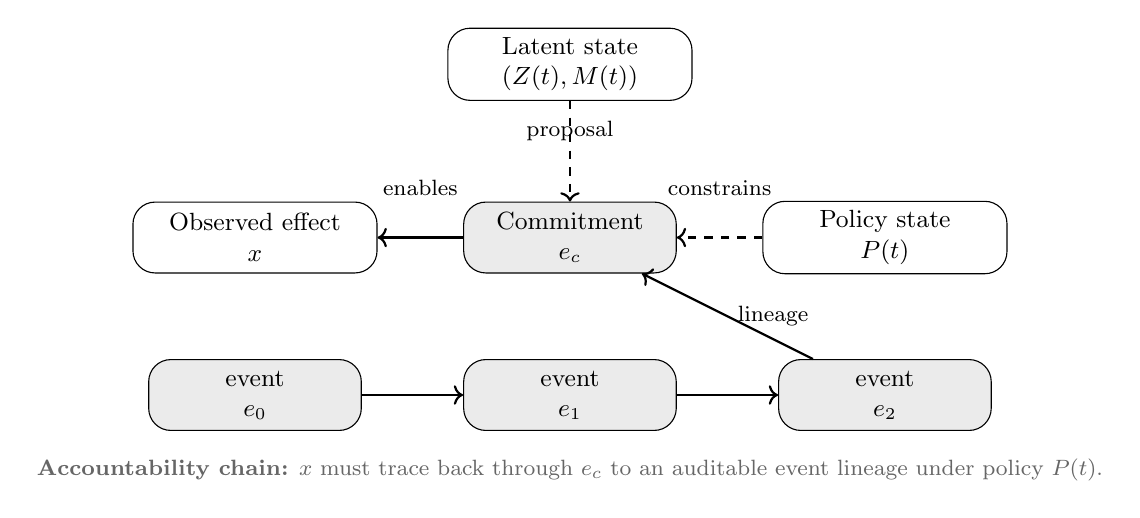
\begin{tikzpicture}[
  font=\small,
  box/.style={draw, rounded corners=8pt, align=center, minimum width=3.1cm, minimum height=0.9cm},
  event/.style={draw, rounded corners=8pt, align=center, minimum width=2.7cm, minimum height=0.9cm, fill=black!8},
  arrow/.style={->, thick},
  dashedarrow/.style={->, thick, dashed},
  faint/.style={black!60}
]

\node[box]   (obs) at (0,0) {Observed effect\\$x$};
\node[event] (ec)  at (4.0,0) {Commitment\\$e_c$};
\node[box]   (pi)  at (8.0,0) {Policy state\\$P(t)$};
\node[box]   (mem) at (4.0,2.2) {Latent state\\$(Z(t),M(t))$};

\node[event] (e0)  at (0.0,-2.0) {event\\$e_0$};
\node[event] (e1)  at (4.0,-2.0) {event\\$e_1$};
\node[event] (e2)  at (8.0,-2.0) {event\\$e_2$};

\draw[arrow] (ec) -- node[above=4mm]{\footnotesize enables} (obs);
\draw[dashedarrow] (pi) -- node[above=4mm]{\footnotesize constrains} (ec);
\draw[dashedarrow] (mem) -- node[above]{\footnotesize proposal} (ec);

\draw[arrow] (e0) -- (e1);
\draw[arrow] (e1) -- (e2);
\draw[arrow] (e2) -- node[right]{\footnotesize lineage} (ec);

\node[faint, align=left] at (4.0,-2.95)
{\footnotesize \textbf{Accountability chain:} $x$ must trace back through $e_c$ to an auditable event lineage under policy $P(t)$.};

\end{tikzpicture}
\caption{Provenance and accountability chain. World effects must be traceable to explicit commitments and an event lineage consistent with the active policy state.}
\label{fig:provenance-chain}
\end{figure}

\subsection{Containment and Scope Control}
\label{sec:containment}

Because EVOS is open and self-modifying, containment must be defined operationally:

\begin{itemize}
  \item \textbf{Scope:} which action families are even eligible for commitment (capability contracts).
  \item \textbf{Budget:} hard resource envelopes (time/compute/money/permissions).
  \item \textbf{Blast radius:} staged rollout for operator or policy changes (canary \& rollback).
  \item \textbf{Observation:} mandatory telemetry + immutable logs for external effects.
\end{itemize}

These are not ``controls around AI''; they are part of the EVOS transition law.

\subsection{Ethical Diversity and Pluralism}
\label{sec:pluralism}

Ethics cannot be collapsed into a single scalar objective without encoding the biases of that scalar.
EVOS therefore supports \emph{constraint sets} and \emph{governance modes}:

\[
\mathcal{C}(t) \in \{\mathcal{C}^{(1)}(t),\ldots,\mathcal{C}^{(m)}(t)\},
\]
with mode changes requiring explicit policy events $e_P$. Pluralism does not remove conflict;
it makes conflict \emph{explicit, auditable, and governable}.

\subsection{Failure Modes and Mitigation}
\label{sec:failure-modes}

EVOS highlights distinctive failure modes:

\begin{itemize}
  \item \textbf{Commitment leakage:} world effects without explicit $e_c$ (broken boundary).
  \item \textbf{Policy drift without lineage:} $P(t)$ changes without $e_P$ (ungoverned updates).
  \item \textbf{Operator mutation without audit:} $\Theta$ shifts without event anchors (unaccountable self-modification).
  \item \textbf{Constraint gaming:} optimizing proxies that satisfy checks but violate intent (specification failure).
\end{itemize}

Mitigations are structural: enforce commitment gates, event-anchored policy/ops lineage, regression invariants,
and staged rollout with automatic rollback.

\subsection{Why Governance Completes EVOS}
\label{sec:why-governance}

Governance completes EVOS because it provides the missing half of open-ended intelligence:
\emph{what persists must be accountable}. Commitment makes consequences real; selection makes them matter
(Section~\ref{sec:learning-selection}); governance ensures they remain bounded, auditable, and socially legible
over time.

%%%%%%%%%%%%%%%%%%%%%%%%%%%%%%%%%%%%%%%%%%%%%%%%%

\section{Applications and Impact}
\label{sec:applications}

EVOS is a theory of intelligence as \emph{worldline evolution under constraint}. Its practical
value is that it turns vague desiderata (``aligned agents'', ``accountable autonomy'',
``adaptive systems'') into \emph{structural requirements}: commitment boundaries, provenance,
pluggable evolution laws, and explicit constraint dynamics.

This section makes three explicit claims:

\begin{enumerate}
  \item \textbf{EVOS is applicative by construction:} any domain with irreversible effects and adaptation benefits from commitment/provenance semantics.
  \item \textbf{EVOS unifies scales:} the same primitives describe single agents, institutions, and substrate-hybrid systems.
  \item \textbf{EVOS changes what is optimized:} from snapshot metrics to trajectory stability and bounded consequence.
\end{enumerate}

\subsection{AI Agent Civilizations}


EVOS is a substrate for \emph{multi-agent civilizations} rather than a single-domain application. Within such civilizations, an economy is not an optional add-on: it is a \emph{civilization kernel}---a persistent coordination layer that allocates scarce capacity (resources, attention, energy, time) under evolving constraints. In EVOS terms, ``finance'' is the canonical high-stakes instantiation of the substrate primitives:
\begin{itemize}
    \item \textbf{Worldline primacy $\rightarrow$ trajectory-based identity, credit, and risk.} Creditworthiness is a property of an agent's historically grounded worldline (commitment history, constraint compliance, failure recovery), not a snapshot score.
    \item \textbf{Commitment boundary $\rightarrow$ settlement and irreversibility.} Financial actions are \emph{externally binding} world-effects; they must cross an explicit commitment gate that compiles policy and invariants into a verifiable commitment event.
    \item \textbf{Intrinsic memory $\rightarrow$ causal provenance and audit without reconstruction.} The ledger is not an after-the-fact archive; it is the living memory of commitments and consequences, enabling structural accountability.
    \item \textbf{Projection $\rightarrow$ privacy and competition.} Agents may keep strategies and intent latent while exposing only minimal, policy-compliant projections to counterparties and the environment (selective revelation under dispute).
    \item \textbf{Openness-under-constraint $\rightarrow$ regulation as physics.} Compliance is enforced as substrate constraints and feasibility boundaries rather than external ``policing,'' enabling continuous markets with built-in homeostasis.
    \item \textbf{Operator evolution $\rightarrow$ adaptive market rules without history reset.} Governance can update transition operators (within constraint envelopes) while preserving worldline continuity and provenance.
\end{itemize}
A complete EVOS-native financial system (exchange, banking, insurance, regulation-by-constraint) is developed as a dedicated companion work (e.g., \emph{EVOS Financial System / ERX / EFF / ORS}) that serves as a proof-by-construction of these primitives in a safety-critical, adversarial domain.


\label{sec:app-civilizations}

Multi-agent systems become qualitatively different when agents are persistent and accountable.
In EVOS, an ``agent society'' is a resonance field over agent worldlines with institution-like
constraints and commitment-mediated interaction. The key contribution is not coordination per se,
but \emph{institutional legibility}: actions are commitments with lineage.

\begin{itemize}
  \item \textbf{Roles} emerge as stable attractors in the resonance field (persistent interaction motifs).
  \item \textbf{Institutions} are constraint regimes $\mathcal{C}^{(k)}(t)$ with explicit policy events.
  \item \textbf{Culture} is a long-timescale memory field shaping feasible commitments.
\end{itemize}


%%%%%%%%%%%%%%%%%%%%%%%%%%%%%%%%%%%%%%%%%%%%%%%%
% Figure: Agent civilization layers in EVOS (compact)
% Requires: \usetikzlibrary{positioning,calc}
%%%%%%%%%%%%%%%%%%%%%%%%%%%%%%%%%%%%%%%%%%%%%%%%
\begin{figure}[t]
\centering
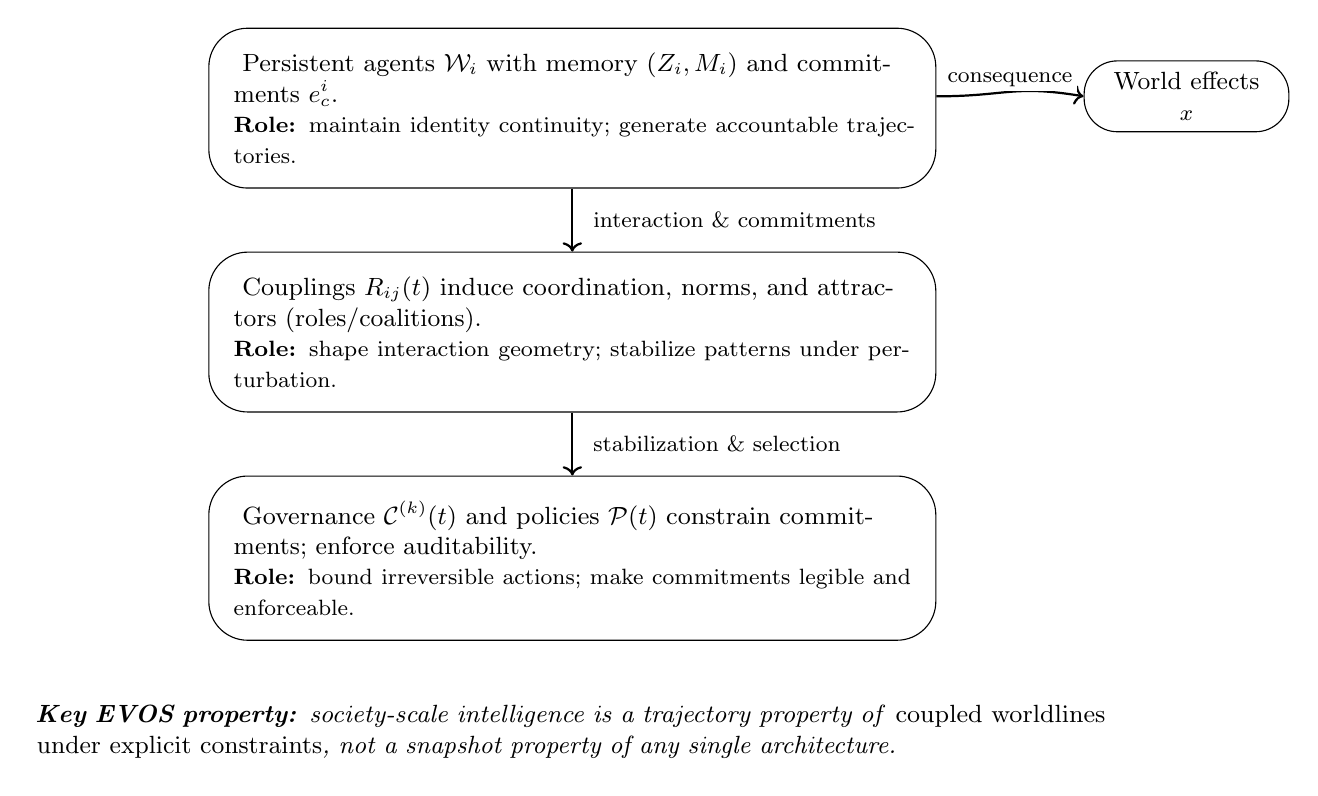
\begin{tikzpicture}[
  font=\small,
  box/.style={
    draw, rounded corners=14pt,
    align=left,
    minimum width=9.2cm,
    text width=8.6cm,
    inner sep=9pt
  },
  title/.style={font=\bfseries},
  arrow/.style={->, thick},
  note/.style={font=\small\itshape, align=left, text width=13.6cm},
  lab/.style={font=\footnotesize, fill=white, inner sep=1.5pt},
  xbox/.style={draw, rounded corners=12pt, align=center, minimum width=2.6cm, minimum height=0.9cm}
]

% --- Three layers (stacked, compact text) ---
\node[box] (W) at (0,0) {%
  \title{Worldline layer.} Persistent agents $\mathcal{W}_i$ with memory $(Z_i,M_i)$ and commitments $e_c^i$.\\
  \footnotesize \textbf{Role:} maintain identity continuity; generate accountable trajectories.%
};

\node[box, below=8mm of W] (R) {%
  \title{Resonance layer.} Couplings $R_{ij}(t)$ induce coordination, norms, and attractors (roles/coalitions).\\
  \footnotesize \textbf{Role:} shape interaction geometry; stabilize patterns under perturbation.%
};

\node[box, below=8mm of R] (I) {%
  \title{Institution layer.} Governance $\mathcal{C}^{(k)}(t)$ and policies $\mathcal{P}(t)$ constrain commitments; enforce auditability.\\
  \footnotesize \textbf{Role:} bound irreversible actions; make commitments legible and enforceable.%
};

% --- Vertical arrows + labels ---
\draw[arrow] (W.south) -- node[lab, midway, right=2mm] {interaction \& commitments} (R.north);
\draw[arrow] (R.south) -- node[lab, midway, right=2mm] {stabilization \& selection} (I.north);

% --- Side callout: world effects (kept small + non-overlapping) ---
\node[xbox] (X) at (7.8,0.15) {World effects\\\footnotesize $x$};
\draw[arrow] ($(W.east)+(0,0.15)$) .. controls +(0.9,0.0) and +(-0.9,0.15) ..
  node[lab, above]{consequence} (X.west);

% --- Key property statement ---
\node[note, below=7mm of I, anchor=north] (K) {%
\textbf{Key EVOS property:} society-scale intelligence is a trajectory property of \emph{coupled worldlines under explicit constraints}, not a snapshot property of any single architecture.%
};

\end{tikzpicture}
\caption{Agent civilization layers in EVOS: persistent worldlines, resonance coupling, and institutional constraints with commitment/provenance semantics.}
\label{fig:agent-civ-layers}
\end{figure}

%%%%%%%%%%%%%%%%%%%%%%%%%%%%%%%%%%%%%%%%%%%
% Figure: Digital EVOS agent civilization architecture (clean layout)
% Requires: \usetikzlibrary{positioning,calc,fit,arrows.meta}
%%%%%%%%%%%%%%%%%%%%%%%%%%%%%%%%%%%%%%%%%%%
\begin{figure}[t]
\centering
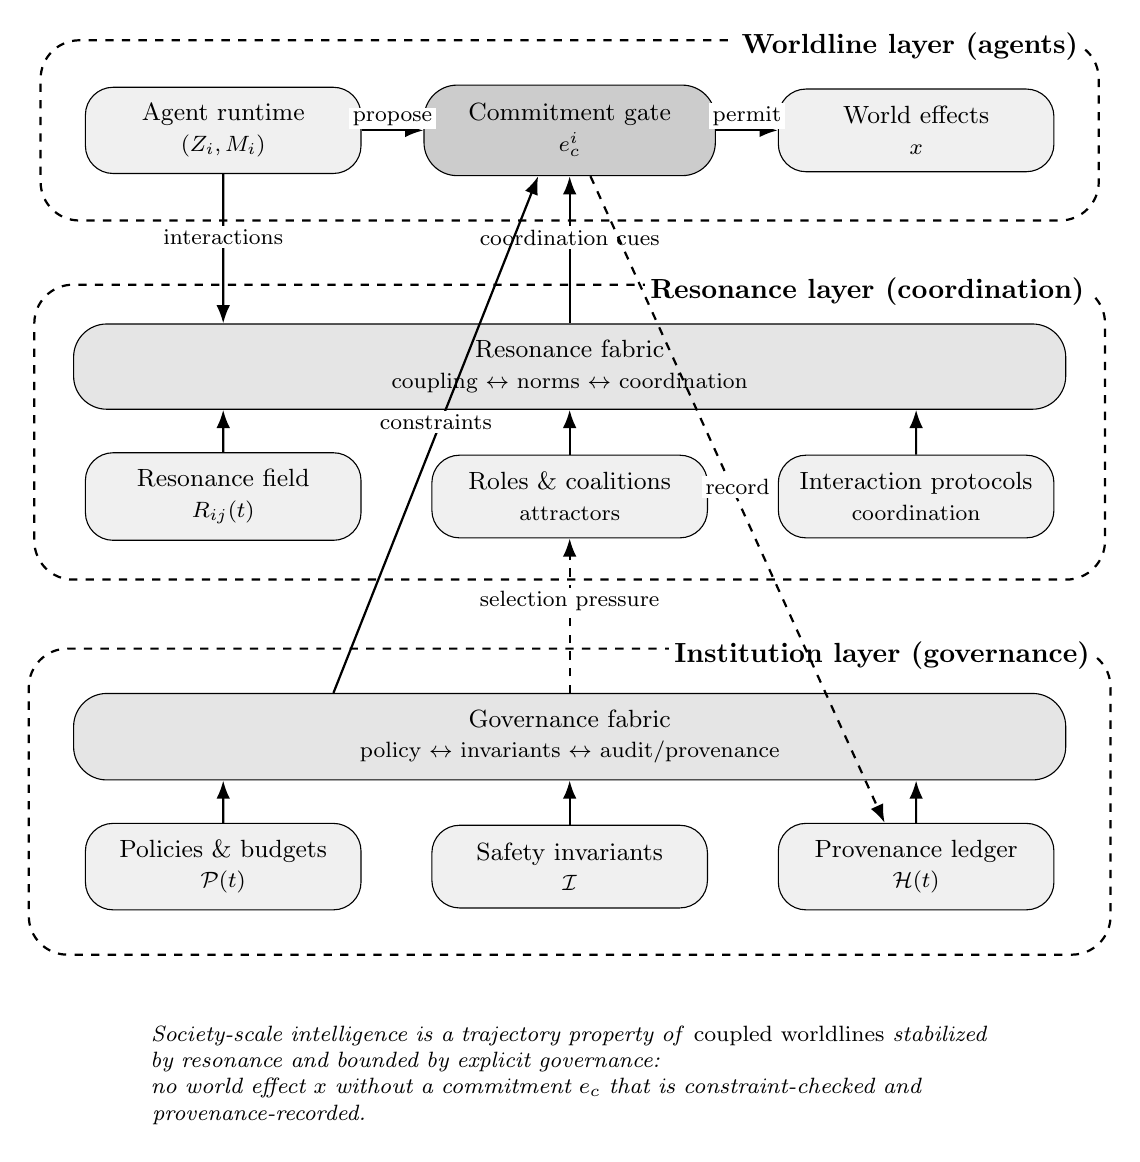
\begin{tikzpicture}[
  font=\small,
  % --- styles ---
  frame/.style={draw, rounded corners=14pt, thick, dashed},
  layerlabel/.style={font=\bfseries, fill=white, inner sep=2pt},
  service/.style={
    draw, rounded corners=10pt, fill=black!6,
    align=center, minimum height=1.05cm, minimum width=3.5cm, inner sep=6pt
  },
  gate/.style={
    draw, rounded corners=12pt, fill=black!20,
    align=center, minimum height=1.15cm, minimum width=3.7cm, inner sep=6pt
  },
  bus/.style={
    draw, rounded corners=12pt, fill=black!10,
    align=center, minimum height=0.95cm, minimum width=12.6cm, inner sep=6pt
  },
  arrow/.style={-Latex, thick},
  darrow/.style={-Latex, thick, dashed},
  lab/.style={font=\footnotesize, fill=white, inner sep=1.3pt}
]

% ======================================================
% Coordinates (one clean vertical stack; no overlaps)
% ======================================================
% Top row (agents)
\node[service] (agent) at (-4.4, 3.75) {Agent runtime\\\footnotesize $(Z_i, M_i)$};
\node[gate]    (cg)    at ( 0.0, 3.75) {Commitment gate\\\footnotesize $e_c^i$};
\node[service] (world) at ( 4.4, 3.75) {World effects\\\footnotesize $x$};

% Resonance bus + middle services
\node[bus]     (rbus)  at ( 0.0, 0.75) {Resonance fabric\\\footnotesize coupling $\leftrightarrow$ norms $\leftrightarrow$ coordination};
\node[service] (field) at (-4.4, -0.9) {Resonance field\\\footnotesize $R_{ij}(t)$};
\node[service] (roles) at ( 0.0, -0.9) {Roles \& coalitions\\\footnotesize attractors};
\node[service] (proto) at ( 4.4, -0.9) {Interaction protocols\\\footnotesize coordination};

% Governance bus + bottom services
\node[bus]     (gbus)  at ( 0.0,-3.95) {Governance fabric\\\footnotesize policy $\leftrightarrow$ invariants $\leftrightarrow$ audit/provenance};
\node[service] (pol)   at (-4.4,-5.6) {Policies \& budgets\\\footnotesize $\mathcal{P}(t)$};
\node[service] (inv)   at ( 0.0,-5.6) {Safety invariants\\\footnotesize $\mathcal{I}$};
\node[service] (prov)  at ( 4.4,-5.6) {Provenance ledger\\\footnotesize $\mathcal{H}(t)$};

% ======================================================
% Layer frames + labels (fit around each region)
% ======================================================
\node[frame, fit=(agent)(cg)(world), inner sep=16pt] (Fagents) {};
\node[frame, fit=(rbus)(field)(roles)(proto), inner sep=14pt] (Fres) {};
\node[frame, fit=(gbus)(pol)(inv)(prov), inner sep=16pt] (Fgov) {};

\node[layerlabel, anchor=east] at ($(Fagents.north east)+(-0.2,-0.1)$) {Worldline layer (agents)};
\node[layerlabel, anchor=east] at ($(Fres.north east)+(-0.2,-0.1)$) {Resonance layer (coordination)};
\node[layerlabel, anchor=east] at ($(Fgov.north east)+(-0.2,-0.1)$) {Institution layer (governance)};

% ======================================================
% Intra-agent flow
% ======================================================
\draw[arrow] (agent) -- node[lab, above] {propose} (cg);
\draw[arrow] (cg) -- node[lab, above] {permit} (world);

% ======================================================
% Resonance fabric hookups (downward + upward cues)
% ======================================================
\draw[arrow] (field.north) -- ([xshift=-44mm]rbus.south);
\draw[arrow] (roles.north) -- (rbus);
\draw[arrow] (proto.north) -- ([xshift=44mm]rbus.south);

\draw[arrow] (agent.south) -- node[lab, above] {interactions}  ([xshift=-44mm]rbus.north);
\draw[arrow] (rbus.north) -- node[lab, above] {coordination cues} (cg.south);

% ======================================================
% Governance fabric hookups
% ======================================================
\draw[arrow] (pol.north) -- ([xshift=-44mm]gbus.south);
\draw[arrow] (inv.north) -- (gbus.south);
\draw[arrow] (prov.north) -- ([xshift=44mm]gbus.south);

% constraints into commitment gate (clean vertical)
\draw[arrow] ([xshift=-3cm]gbus.north) -- node[lab, above] {constraints} ([xshift=-4mm]cg.south);

% provenance recording (dashed, to avoid clutter)
\draw[darrow] (cg) -- node[lab, above] {record} ([xshift=-4mm]prov.north);

% selection pressure into roles/coalitions (dashed, secondary)
\draw[darrow] (gbus.north) -- node[lab, above] {selection pressure} (roles.south);

% ======================================================
% Key property note (kept away from frames)
% ======================================================
\node[align=left, font=\footnotesize\itshape, text width=10.6cm] at (0,-8.25)
{Society-scale intelligence is a trajectory property of \emph{coupled worldlines} stabilized by resonance and bounded by explicit governance:\\
no world effect $x$ without a commitment $e_c$ that is constraint-checked and provenance-recorded.};

\end{tikzpicture}
\caption{Digital EVOS system architecture: agents (worldlines) propose actions; explicit commitments authorize world effects; resonance fabric induces coordination; governance fabric enforces constraints and auditability via provenance.}
\label{fig:digital-evos-architecture}
\end{figure}
%%%%%%%%%%%%%%%%%%%%%%%%%%%%%%%%%%%%%%%%%%%%%%%%


\subsection{Scientific Discovery and Hypothesis Exploration}
\label{sec:app-science}

Scientific discovery is an EVOS domain because it is open, time-extended, and consequence-bearing:
experiments consume resources and irreversibly update shared knowledge. EVOS provides:
(i) persistent memory worldlines for hypotheses and instruments, (ii) commitment-gated experiments,
and (iii) provenance lineage from evidence to claims.

A hypothesis becomes a worldline $\mathcal{W}_h$ whose commitments are experimental actions; its
``fitness'' is stability under constraint (reproducibility, cost, ethical bounds).

\subsection{Medicine and Personalized Biology}
\label{sec:app-medicine}

Personalized medicine is trajectory-dominated: interventions alter future physiology irreversibly.
EVOS recommends commitment-gated clinical actions with explicit policy constraints (protocols,
consent, safety) and provenance from measurements $\rightarrow$ diagnosis $\rightarrow$ intervention.
Hybrid BIO-EVOS systems naturally fit: molecular dynamics provide substrate-level memory and
constraints (kinetics, scarcity), while digital agents provide deliberation and audit.

\subsection{Optimization Beyond Objective Functions}
\label{sec:app-optimization}

Standard optimization presumes a fixed objective; EVOS reframes optimization as maintaining
bounded trajectory under evolving constraints:
\[
\text{minimize violations of } \Phi(\mathcal{W}) \text{ subject to } \mathcal{C}(t), \text{ with commitments anchored in } \mathcal{H}(t).
\]
This supports multi-stakeholder systems where objectives conflict and policies evolve.

\subsection{Knowledge Preservation and Long-Term Memory}
\label{sec:app-memory}

EVOS supports persistent, provenance-aware knowledge: rather than storing static documents, it
stores \emph{lineage} (why beliefs changed, which commitments were made, and which evidence anchors exist).
This is critical for institutional memory and long-horizon alignment.

\subsection{Societal-Scale Governance Systems}
\label{sec:app-governance}

EVOS provides a formal substrate for governance automation without collapsing governance into
a single score: policy is an evolving constraint process with explicit mode changes, audits,
and rollback. This enables accountable ``agentic bureaucracy'' where commitments are legible
and reversible actions are maximized, irreversible actions minimized and justified.

\subsection{Impact on the Theory of Computation}
\label{sec:impact-toc}

EVOS does not refute the Church--Turing thesis; it changes the \emph{object of study}.
Turing computation characterizes what can be computed as a function. EVOS characterizes what
can be sustained as a \emph{bounded, accountable trajectory} in an open world.


%%%%%%%%%%%%%%%%%%%%%%%%%%%%%%%%%%%%%%%%%%%%%%%%%%%%%
\section{Discussion, Limitations, and Future Directions}
\label{sec:discussion}

A Turing-grade theory must state its limits clearly. EVOS is a structural theory; it does not
provide a closed-form algorithm for intelligence. It specifies \emph{necessary primitives} and
\emph{admissible dynamics} for accountable open-ended systems.

\subsection{Related Work and Historical Positioning}

EVOS is deliberately \emph{not} proposed as a competing neural architecture.
It is a \emph{systems-class} and \emph{accountability formalism} for persistent,
open, history-bearing computation. In this sense, EVOS sits at the intersection
of (i) classical computation and its limits \cite{turing1936,church1936},
(ii) interaction and non-terminating computation \cite{wegner1997},
(iii) cybernetics and control under feedback \cite{wiener1948,kalman1960},
(iv) dynamical systems and stability under constraint \cite{strogatz1994},
and (v) biological autonomy and self-production \cite{maturana1980}.

Several themes are closest in spirit but differ in emphasis. First, interactive
computation frameworks argue that \emph{ongoing interaction} extends the expressive
concerns of classical, input--output machines \cite{wegner1997}; EVOS adds the
missing \emph{commitment boundary} as a structural requirement for real-world
accountability. Second, dynamical systems and control theory provide the mathematics
of trajectories, attractors, and stability \cite{strogatz1994,kalman1960}; EVOS
uses these tools but elevates \emph{irreversibility and provenance} to first-class
constraints. Third, reaction--diffusion and morphogenesis show how stable patterns
emerge from local interactions \cite{turing1952}; EVOS reinterprets these patterns
as \emph{resonant} structures that can encode memory, norm, and institution at
multiple scales. Finally, reinforcement learning formalizes adaptation under reward
\cite{sutton2018}; EVOS generalizes beyond reward to \emph{constraint compatibility}
and commitment-scoped external consequences.

EVOS can be read as a synthesis: the Church--Turing thesis abstracts \emph{computation}
away from machines; EVOS abstracts \emph{intelligence-under-time} away from architectures.
This shifts the scientific question from ``what function is computed?'' to ``what
trajectories are stabilized, under what constraints, and with what accountable
consequences?''

\subsection{Positioning EVOS in the History of Computation}
\label{sec:position-history}

EVOS is to intelligence what process calculi and systems theory are to programs: it focuses on
interaction, persistence, and evolution. Where Turing machines formalize computation-as-function,
EVOS formalizes intelligence-as-trajectory with commitment semantics.

\subsection{Relationship to Existing AI Architectures}
\label{sec:relation-architectures}

Transformers, planners, RL agents, and symbolic systems can all be embedded in EVOS as internal
modules. EVOS is orthogonal: it governs how internal cognition becomes external effect, how
memory persists, and how evolution laws change under constraint.

\subsection{Conceptual Limitations}
\label{sec:concept-limits}

\begin{itemize}
  \item \textbf{Not sufficient:} EVOS axioms are necessary conditions, not a recipe for intelligence.
  \item \textbf{Constraint selection:} choosing $\mathcal{C}(t)$ and $\Phi$ is a normative problem.
  \item \textbf{Measurement limits:} provenance depends on observability; some substrates are partially observable.
\end{itemize}

\subsection{Practical Limitations}
\label{sec:practical-limits}

\begin{itemize}
  \item \textbf{Overhead:} commitment/provenance infrastructure adds latency and complexity.
  \item \textbf{Specification gaps:} policy predicates can be incomplete or gameable.
  \item \textbf{Scaling:} lineage graphs and logs require efficient summarization and verification.
\end{itemize}

\subsection{Epistemic Limits}
\label{sec:epistemic-limits}

Open systems face fundamental epistemic uncertainty: the environment is not fully modelable.
EVOS addresses this by making uncertainty explicit at the commitment boundary, but it does not
eliminate it. The best possible guarantee is bounded consequence under explicit uncertainty.

\subsection{Open Research Questions}
\label{sec:open-questions}

\begin{enumerate}
  \item \textbf{Trajectory metrics:} principled forms of $\Phi(\mathcal{W})$ capturing safety, coherence, and utility.
  \item \textbf{Policy compilation:} translating legal/ethical norms into auditable predicates $\mathrm{Allow}(\cdot)$.
  \item \textbf{Lineage compression:} provably safe summarization of causal history for scale.
  \item \textbf{Field learning:} formal links between resonance-field plasticity and operator meta-dynamics.
  \item \textbf{Hybrid semantics:} cross-substrate commitment equivalence and measurement trust models.
\end{enumerate}

\subsection{Risks and Misuse Considerations}
\label{sec:misuse}

EVOS can be misused to build more persistent and strategic agents. The mitigation is not to
avoid EVOS, but to insist that persistence comes with enforceable boundaries: explicit
commitments, provenance, budgets, and governance modes. ``Unbounded autonomy'' is precisely the
failure mode EVOS forbids.

\subsection{Why EVOS Is Not Just a Framework}
\label{sec:not-just-framework}

EVOS makes falsifiable structural claims: if a system produces world effects without commitment
events and causal lineage, it violates EVOS; if it cannot represent time as worldline history,
it violates EVOS; if it cannot evolve under explicit constraints, it violates EVOS. These are
not implementation preferences; they are definitional.

\subsection{Future Trajectories}
\label{sec:future}

Immediate directions:
\begin{itemize}
  \item \textbf{Reference implementations} of commitment gating, provenance logs, and operator hot-swap buses.
  \item \textbf{Benchmarks} defined on trajectory stability and bounded consequence rather than task snapshots.
  \item \textbf{Formal verification} of invariants at the commitment boundary (safety regression invariants).
\end{itemize}

%%%%%%%%%%%%%%%%%%%%%%%%%%%%%%%%%%%%%%%%%%%%%%%%%%
\section{Conclusion}
\label{sec:conclusion}

We introduced \textbf{Evolutionary Open Systems (EVOS)}: a class of computational systems defined
axiomatically by worldline primacy, intrinsic memory, openness under constraint, commitment as
a reality boundary, and substrate independence. We introduced \textbf{GENESIS} as a resonance-field
formalism compatible with EVOS, and we developed a pluggable transition mathematics stack spanning
Markov models, time-series dynamics, differential/reaction--diffusion systems, and learned/self-modifying
operators—each constrained by explicit commitments and causal provenance.

The central thesis is simple and structural:

\begin{quote}
\emph{Intelligence in the real world is not a snapshot computation. It is an accountable,
constraint-bounded trajectory that persists through irreversible time.}
\end{quote}

EVOS therefore shifts the ground of AI from architecture-centric optimization to trajectory-centric
systems engineering: commitments define reality, provenance defines accountability, and constraints define
what it means for evolution to be intelligent rather than merely powerful.

%%%%%%%%%%%%%%%%%%%%%%%%%%%%%%%%%%%%%%%%%%%%%%%%%%%%%




%==============================================================================
% Appendix: Figure Index
%==============================================================================
\appendix
\section{Figure Index}
\label{app:figure-index}

% If your class/style already prints a List of Figures elsewhere, you can remove this.
\listoffigures

\noindent
This appendix provides a consolidated index of figures for reviewers. Figure captions are
the authoritative descriptions of each artifact; cross-references in the main text use
standard \LaTeX\ labels to remain stable under restructuring.


\begin{thebibliography}{99}

\bibitem{turing1936}
A.~M. Turing.
\newblock On computable numbers, with an application to the {E}ntscheidungsproblem.
\newblock \emph{Proceedings of the London Mathematical Society}, 2(42):230--265, 1936.

\bibitem{church1936}
A.~Church.
\newblock An unsolvable problem of elementary number theory.
\newblock \emph{American Journal of Mathematics}, 58(2):345--363, 1936.

\bibitem{wegner1997}
P.~Wegner.
\newblock Why interaction is more powerful than algorithms.
\newblock \emph{Communications of the ACM}, 40(5):80--91, 1997.

\bibitem{wiener1948}
N.~Wiener.
\newblock \emph{Cybernetics: Or Control and Communication in the Animal and the Machine}.
\newblock MIT Press, 1948.

\bibitem{kalman1960}
R.~E. Kalman.
\newblock A new approach to linear filtering and prediction problems.
\newblock \emph{Journal of Basic Engineering}, 82(1):35--45, 1960.

\bibitem{strogatz1994}
S.~H. Strogatz.
\newblock \emph{Nonlinear Dynamics and Chaos}.
\newblock Westview Press, 1994.

\bibitem{maturana1980}
H.~R. Maturana and F.~J. Varela.
\newblock \emph{Autopoiesis and Cognition: The Realization of the Living}.
\newblock D. Reidel, 1980.

\bibitem{turing1952}
A.~M. Turing.
\newblock The chemical basis of morphogenesis.
\newblock \emph{Philosophical Transactions of the Royal Society of London. Series B},
237(641):37--72, 1952.

\bibitem{sutton2018}
R.~S. Sutton and A.~G. Barto.
\newblock \emph{Reinforcement Learning: An Introduction}.
\newblock MIT Press, 2nd edition, 2018.

\bibitem{markov1906}
A.~A. Markov.
\newblock Extension of the law of large numbers to dependent quantities.
\newblock \emph{Izvestiya Fiziko-Matematicheskogo Obshchestva}, 15:135--156, 1906.

\end{thebibliography}

\end{document}